\documentclass[
	11pt,
	openright,
	oneside,
	a4paper,
	english,
	french,	
	spanish,
	brazil,
	]{abntex2}

\usepackage{abntex2-cefetmg-timoteo}
\usepackage{cmap}				
\usepackage{lmodern}			
\usepackage[T1]{fontenc}		
\usepackage[utf8]{inputenc}		
\usepackage{lastpage}			
\usepackage{indentfirst}		
\usepackage{color}				
\usepackage{graphicx}
% Permite nomes de arquivos com espacos, multiplos pontos e caracteres estendidos
\usepackage{grffile}
\PassOptionsToPackage{normalem}{ulem} 
\usepackage{ulem}
\usepackage{multicol}
\usepackage{courier}
\usepackage{listings, xcolor}

\lstset{
tabsize = 4,
showstringspaces = false, 
numbers = left, 
commentstyle = \color{green},
keywordstyle = \color{blue},
stringstyle = \color{green},
rulecolor = \color{black}, 
basicstyle = \small \ttfamily,
breaklines = true,
numberstyle = \tiny,
}
\usepackage{helvet}
\renewcommand{\familydefault}{\sfdefault}
\usepackage[brazilian,hyperpageref]{backref}
\usepackage[alf,abnt-thesis-year=both]{abntex2cite}
\usepackage{longtable}
\usepackage{tikz}
\usetikzlibrary{shapes.geometric, positioning}
\usepackage{array}					
\usepackage{soul}					
\usepackage[framemethod=default]{mdframed}	
\usepackage{pdflscape}				

% Inclui tanto a pasta fig/ quanto a pasta Telas/ e a raiz nas buscas de imagem
\graphicspath{{fig/}{Telas/}{./}}

\definecolor{marcatexto}{rgb}{1,1,0}
\sethlcolor{marcatexto}
\newcommand{\obs}[1]{\hl{#1}}

\newmdenv[
	linewidth=0.6pt,
	linecolor=black,
	backgroundcolor=white,
	innertopmargin=8pt,
	innerbottommargin=8pt,
	innerleftmargin=10pt,
	innerrightmargin=10pt,
	skipabove=\baselineskip,
	skipbelow=\baselineskip
]{casodeuso}

\renewcommand{\labelitemi}{$\bullet$}
\renewcommand{\labelitemii}{$\circ$}

\renewcommand{\backrefpagesname}{Citado na(s) página(s):~}
\renewcommand{\backref}{}
\renewcommand*{\backrefalt}[4]{
	\ifcase #1 %
		Nenhuma citação no texto.%
	\or
		Citado na página #2.%
	\else
		Citado nas páginas #2.%
	\fi}%

\titulo{Documentação do Software: Sistema de Gestão de Empresa Junior}
\autor{Luan Lana Maia \\ Yuri Espindola}
\local{Timóteo - MG}
\data{\today}
\orientador{Márcia}
\instituicao{%
  Centro Federal de Educação Tecnológica de Minas Gerais
  \par
  Campus Timóteo
  \par
  Graduação em Engenharia de Computação
}
\tipotrabalho{Documentação de Software}

\preambulo{Documento apresentado à disciplina de Laboratório de Modelagem de Sistemas do Campus Timóteo do Centro Federal de Educação Tecnológica de Minas Gerais.}

\makeatletter
\hypersetup{
		pdftitle={\@title},
		pdfauthor={\@author},
    	pdfsubject={},
	    pdfcreator={LaTeX with abnTeX2},
		pdfkeywords={abnt}{latex}{abntex}{abntex2}{trabalho acadêmico},
		colorlinks=true,
    	linkcolor=black,
    	citecolor=black,
    	filecolor=black,
		urlcolor=black,
		bookmarksdepth=4
}
\makeatother

\setlength{\parindent}{1.3cm}
\setlength{\parskip}{0.2cm}

\makeindex

\begin{document}
\frenchspacing

\pretextual
\imprimircapa

\renewcommand*{\insertchapterspace}{} 
 
\pdfbookmark[0]{\contentsname}{toc}
\tableofcontents*
\cleardoublepage

\textual
% ----------------------------------------------------------
% 1. Glossário - Definições e Siglas
% ----------------------------------------------------------
\chapter{Glossário -- Definições e Siglas}
\label{cap:glossario}

\section*{Siglas e termos da organização e do negócio}

\begin{description}
    \item[\textbf{EJ}] Empresa Júnior --- associação civil sem fins lucrativos gerida por discentes de graduação, prestando serviços e projetos para aprimoramento profissional acadêmico.
    \item[\textbf{Commit Júnior}] Nome da Empresa Júnior dos cursos de Engenharia do CEFET-MG, atuando como organização cliente e contexto de aplicação do sistema.
    \item[\textbf{Squad}] Subgrupo ou time ágil de trabalho alocado dentro de uma diretoria ou gerência técnica da empresa.
    \item[\textbf{RG (Reunião Geral)}] Reunião plenária periódica e institucional obrigatória, convocada para todos os integrantes ativos da empresa júnior.
    \item[\textbf{1-on-1}] Reunião individual de alinhamento e acompanhamento realizada entre dois membros específicos, desvinculada de eventos plenários.
    \item[\textbf{Alumnus}] Status conferido a ex-membros desligados da empresa júnior, preservando seus registros históricos de atuação sem exclusão física do banco de dados.
    \item[\textbf{Agravante}] Fator multiplicador incidente sobre a pontuação de penalidades quando constatada reincidência infracional antes do prazo regular de expiração.
    \item[\textbf{SIGAA}] Sistema Integrado de Gestão de Atividades Acadêmicas --- plataforma oficial do CEFET-MG em que as horas de extensão validadas são registradas pela coordenação de curso.
    \item[\textbf{CPF}] Cadastro de Pessoa Física --- registro documental civil empregado como identificador primário para assegurar a unicidade cadastral no sistema.
    \item[\textbf{SMTP}] \textit{Simple Mail Transfer Protocol} --- protocolo de comunicação em rede utilizado pelo servidor institucional para o despacho automatizado de notificações e relatórios por correio eletrônico.
\end{description}

\section*{Siglas de engenharia de software e modelagem}

\begin{description}
    \item[\textbf{DCU}] Diagrama de Casos de Uso --- representação gráfica estruturada segundo o padrão UML para mapear atores, casos de uso e os limites de escopo funcional do sistema.
    \item[\textbf{UML}] \textit{Unified Modeling Language} --- notação gráfica padronizada para especificação, modelagem e documentação de artefatos de software orientados a objetos.
    \item[\textbf{UC}] Caso de Uso (\textit{Use Case}) --- identificador padronizado atribuído a cada funcionalidade ou serviço executado pela aplicação (ex.: UC-01, UC-02).
    \item[\textbf{RF}] Requisito Funcional --- declaração dos comportamentos, serviços e processamentos de dados que o software deve prover aos usuários.
    \item[\textbf{RNF}] Requisito Não-Funcional --- especificação de critérios de qualidade, restrições e atributos operacionais da solução (tais como segurança, tempo de resposta e portabilidade).
    \item[\textbf{RN}] Regra de Negócio --- preceito normativo, condição lógica ou restrição operacional inerente ao funcionamento da instituição que delimita o sistema.
\end{description}

\section*{Termos técnicos de segurança e arquitetura}

\begin{description}
    \item[\textbf{RBAC}] \textit{Role-Based Access Control} (Controle de Acesso Baseado em Papéis) --- paradigma de segurança em que os privilégios e permissões de acesso às funcionalidades são determinados estritamente pelo perfil funcional exercido pelo usuário.
    \item[\textbf{Hash criptográfico / BCrypt}] Algoritmo matemático unidirecional de derivação com salgamento seguro, utilizado para converter credenciais de senha em cadeias irreversíveis, prevenindo exposição mesmo em vazamentos de dados.
\end{description}

\section*{Terminologia da notação de Casos de Uso (UML)}

\begin{description}
    \item[\textbf{Ator}] Entidade externa ao ambiente computacional (como pessoa, setor ou subsistema de hardware) que interage ativamente com o sistema.
    \item[\textbf{Ator primário}] Papel que dispara e conduz ativamente a interação com o caso de uso visando atender a uma demanda própria.
    \item[\textbf{Ator secundário}] Entidade externa periférica acionada pelo sistema durante a execução do fluxo para auxílio ou registro, sem que tenha iniciado a requisição original.
    \item[\textbf{Caso de uso}] Unidade lógica de comportamento observável que um ator executa para alcançar um resultado mensurável de valor, abstraindo detalhes internos de código.
    \item[\textbf{Generalização (herança)}] Relação estrutural hierárquica na qual um elemento especializado reaproveita e estende atributos e comportamentos do elemento genérico antecedente.
    \item[\textbf{Inclusão (\guillemotleft include\guillemotright)}] Relacionamento de dependência obrigatória no qual a realização de um caso de uso incorpora incondicionalmente a rotina descrita em outro caso de uso acoplado.
    \item[\textbf{Extensão (\guillemotleft extend\guillemotright)}] Relacionamento condicional e opcional que viabiliza a execução complementar de fluxos específicos a partir de pontos de extensão demarcados no caso de uso base.
\end{description}
% ----------------------------------------------------------
% 2. Repositório(s) do projeto
% ----------------------------------------------------------
\chapter{Repositório(s) do projeto}
\label{cap:repositorios}

{https://github.com/luanfrombrazil/Lab-Modelagem-de-Sistemas}

% ==========================================================
% 3. Conteúdos e Materiais de Referência
% ==========================================================
\chapter{Conteúdos e Materiais de Referência}
\label{cap:materiais}

Nesta seção são apresentados os documentos, planilhas e quadros utilizados atualmente pela Commit Júnior na rotina operacional de gestão de membros, horas e controle disciplinar. Tais registros evidenciam as limitações do modelo manual e fundamentam o levantamento de requisitos do novo sistema.

\section{Itens usados atualmente no contexto}

\begin{figure}[!htbp]
    \centering
    \caption[Planilha de Gerenciamento de Membros e Controle Documental]{Planilha de Gerenciamento de Membros e Controle Documental (Google Sheets)}
    \label{fig:ref-membros}
    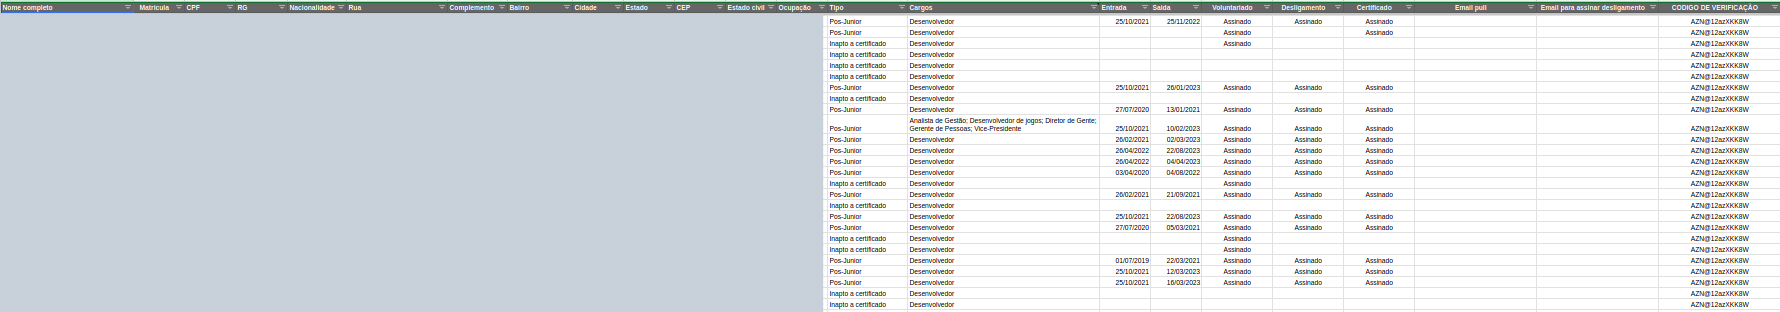
\includegraphics[width=0.95\textwidth]{gerenciamento-de-membros}
\end{figure}
\noindent\textbf{Descrição:} Base gerenciada pelo setor Jurídico e Gestão de Pessoas para controle civil, acadêmico e contratual (termos de voluntariado, desligamento e certificados). Apresenta lacunas de preenchimento, risco de exclusão acidental de linhas e ausência de trilha de auditoria.

\begin{figure}[!htbp]
    \centering
    \caption[Planilha de Gerenciamento e Lançamento de Horas de Extensão]{Planilha de Gerenciamento e Lançamento de Horas de Extensão (Google Sheets)}
    \label{fig:ref-horas}
    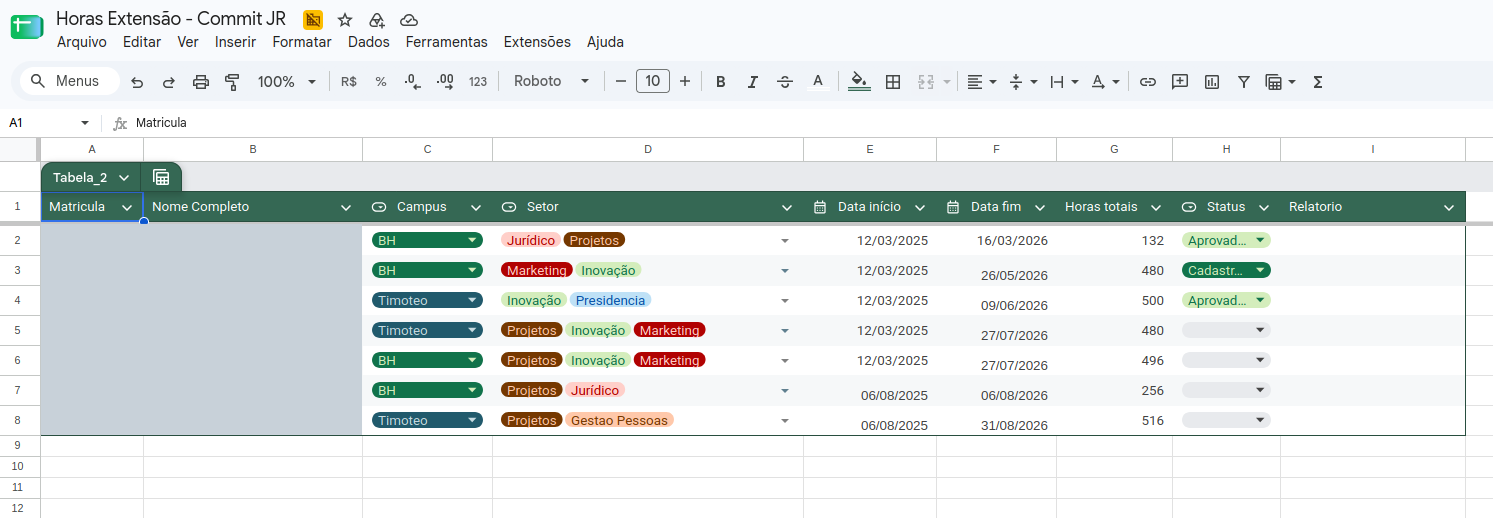
\includegraphics[width=0.95\textwidth]{gerenciamento-de-horas}
\end{figure}
\noindent\textbf{Descrição:} Planilha compartilhada com a coordenação de curso para posterior inserção de horas de extensão no SIGAA. O cômputo do saldo de horas e as notificações de saída de membros dependem de procedimentos manuais e comunicação informal via WhatsApp.

\begin{figure}[!htbp]
    \centering
    \caption[Quadro Geral de Membros e Diretório Corporativo]{Quadro Geral de Membros e Diretório Corporativo (Notion)}
    \label{fig:ref-notion}
    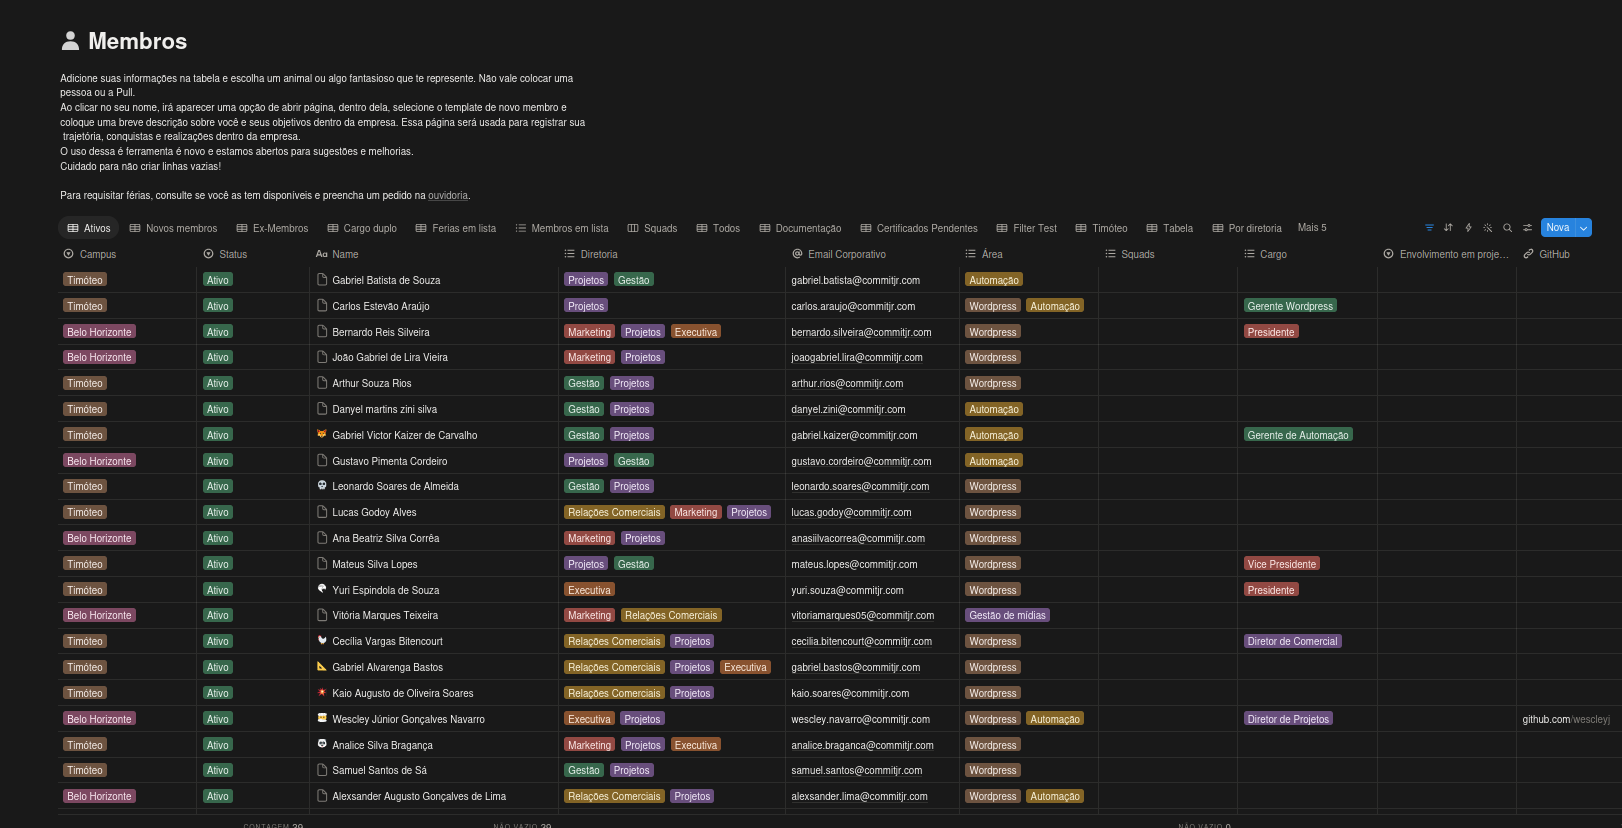
\includegraphics[width=0.95\textwidth]{tela-notion}
\end{figure}
\noindent\textbf{Descrição:} Painel no Notion voltado à consulta interna entre equipes por campus (Timóteo e Belo Horizonte), diretorias, squads e contatos. Sofre com inconsistências cadastrais provocadas pelo esquecimento de atualização e permanência de ex-membros como ativos.

\begin{figure}[!htbp]
    \centering
    \caption[Painel de Lançamento de Pontos e Penalidades]{Painel de Lançamento de Pontos e Penalidades (Notion)}
    \label{fig:ref-pontos}
    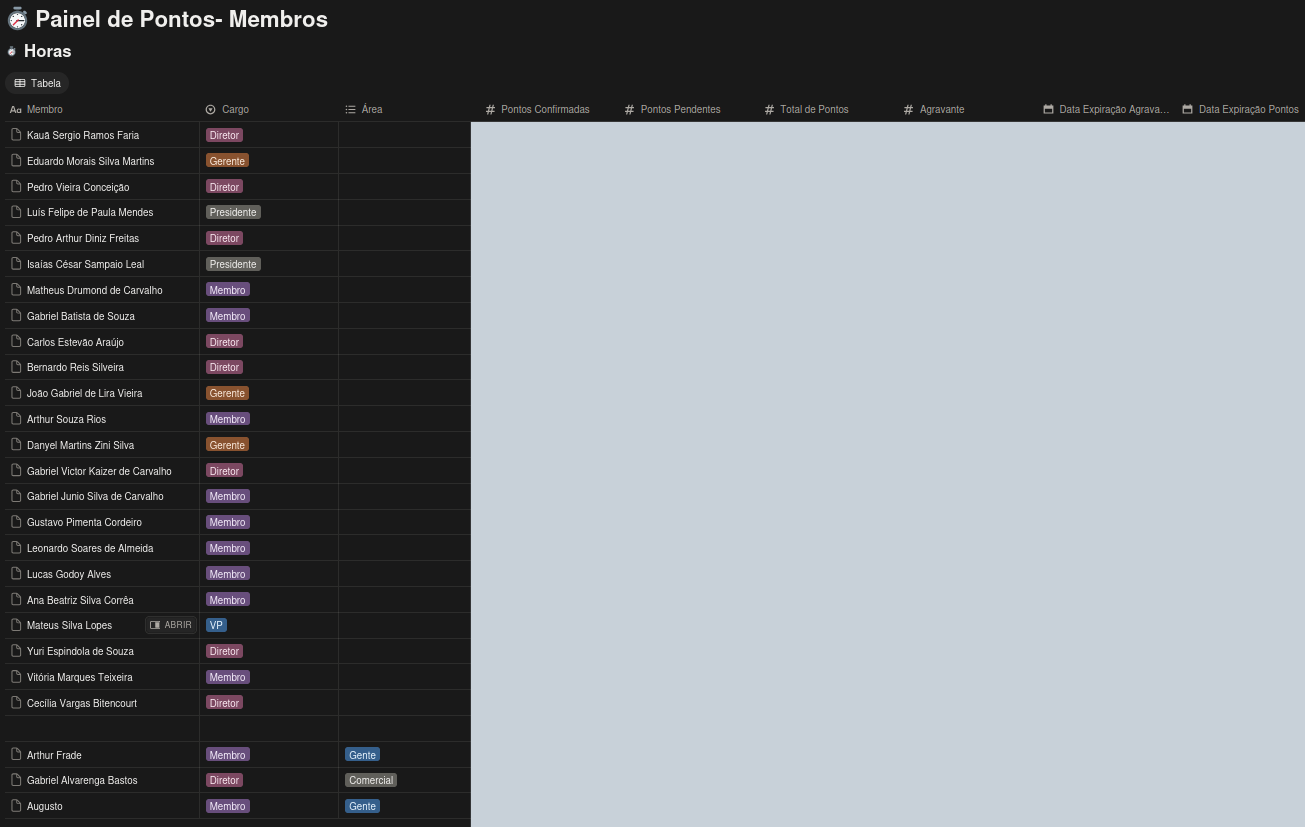
\includegraphics[width=0.95\textwidth]{tela-lancamento-de-pontos}
\end{figure}
\noindent\textbf{Descrição:} Painel para acompanhamento de advertências, agravantes e prazos de validade disciplinar. Possui vulnerabilidade de segurança (permissão aberta para edição por qualquer integrante) e ausência de rotinas automáticas de expiração e reincidência.

\clearpage
% ==========================================================
% 4. Minimundo do Projeto (Contexto atual)
% ==========================================================
\chapter{Minimundo do Projeto (Contexto atual)}
\label{cap:minimundo}

A Commit Júnior é uma Empresa Júnior (EJ) sem fins lucrativos, gerida exclusivamente por discentes de cursos de graduação em Engenharia do Centro Federal de Educação Tecnológica de Minas Gerais (CEFET-MG). A organização atua no mercado fornecendo serviços de consultoria e soluções computacionais, estruturando seu quadro operacional e administrativo em diretorias e gerências especializadas, tais como Diretoria Executiva, Gestão de Pessoas, Jurídico, Comercial e Projetos. Para a realização das atividades diárias, os membros utilizam notebooks, computadores pessoais e smartphones, mantendo a comunicação por meio de redes Wi-Fi acadêmicas nos campi da instituição de ensino, redes residenciais em regime remoto e pacotes de dados móveis com conectividade estável. O corpo de membros é composto por graduandos de 18 a 26 anos, todos plenamente alfabetizados, comunicativos e dotados de alto nível de proficiência técnica no uso de tecnologias digitais e serviços em nuvem.

No fluxo operacional vigente, o gerenciamento de pessoas, a formalização contratual e o controle das rotinas internas dependem de processos descentralizados e manuais, divididos entre diferentes ferramentas e responsáveis:

No âmbito cadastral e contratual, a captação inicial dos dados pessoais e civis dos membros é feita por formulários do Google Forms. Essas respostas são exportadas para planilhas do Google Sheets gerenciadas pelo setor Jurídico. A partir daí, o Jurídico precisa consultar individualmente as linhas da planilha, conferir os dados e gerar manualmente os termos de voluntariado a partir de um modelo padrão, os quais são posteriormente encaminhados para assinatura eletrônica por meio da plataforma Autentique. O controle do retorno dessas assinaturas é registrado manualmente na planilha de membros por meio de códigos de verificação de autenticidade dos termos. O mesmo procedimento manual e moroso se repete quando ocorre a saída de um integrante: o Jurídico redige um termo de desligamento nos mesmos moldes, colhe as assinaturas via Autentique e atualiza o status na planilha. De forma análoga, a emissão e o acompanhamento de certificados de participação na empresa júnior passam por essa conferência manual de registros e preenchimento de modelos para cada membro.

No gerenciamento de extensão acadêmica, a contabilização das horas é mantida em uma planilha específica do Google Sheets. Ao término do ciclo de permanência do membro na empresa, o assessor da presidência realiza o cálculo manual do tempo de casa e da quantidade total de horas de extensão acumuladas em cada cargo desempenhado. Esse cálculo manual toma muito tempo e está sujeito a erros contínuos de contagem e digitação. Concluída a soma, as informações do aluno e o total de horas são enviados de maneira informal pelo WhatsApp para o professor orientador da Commit Júnior. O professor orientador, por sua vez, realiza a inserção desses dados no SIGAA, no qual é lançado o processo de extensão; a partir disso, o membro precisa elaborar e submeter um relatório individual de atividades na plataforma acadêmica para que, após a devida aprovação, receba o certificado de extensão oficial do CEFET-MG.

Paralelamente, a consulta de contatos internos, squad e cargos dos integrantes em exercício é mantida em quadros colaborativos no Notion, ferramenta na qual a liderança também preenche um painel de lançamentos de pontos para controle disciplinar (faltas, advertências e condutas inadequadas). A verificação dos prazos de validade dessas pontuações e o cômputo dos agravantes por reincidência exigem conferência estritamente visual dos gestores, pois a ferramenta não possui automação para caducidade nem para multiplicação de penalidades. Por fim, as Reuniões Gerais (RG) e os alinhamentos bilaterais (1-on-1) são organizados de modo descentralizado por aplicativos de mensagem instantânea e calendários pessoais, resultando frequentemente em sobreposições de agenda e choques com compromissos corporativos obrigatórios.

Essa dinâmica fragmentada gera vulnerabilidades críticas: redundância de retrabalho entre Google Forms, Autentique, Google Sheets e Notion; campos obrigatórios não preenchidos; permanência indevida de ex-membros como ativos nas listagens de consulta; quebra de fórmulas nas planilhas e risco constante de alteração indevida de pontos disciplinares devido à ausência de restrição de acesso. Além disso, a dependência do WhatsApp para notificar o professor orientador sobre horas e desligamentos despersonaliza o processo institucional e provoca atrasos na formalização acadêmica junto ao SIGAA.

Em resposta a essas dificuldades, a Commit Júnior anseia por uma plataforma web integrada que estabeleça controle unificado em todas as suas frentes de gestão de pessoas. A instituição espera que o ambiente implemente autenticação segura com perfis de Administrador, Jurídico, Líderes de Área e Membros. O cliente deseja a centralização completa do cadastro dos membros com histórico imutável, além do gerenciamento dos fluxos e status de assinatura dos termos de voluntariado, termos de desligamento e certificados corporativos. Almeja-se a automação integral do cômputo de horas de extensão e tempo de casa com base nos cargos exercidos, eliminando as contas manuais e possibilitando o envio formalizado de relatórios diretamente por e-mail para o professor orientador da Commit Júnior realizar os registros no SIGAA. Para a governança disciplinar, busca-se um módulo que automatize a expiração de penalidades e a aplicação de agravantes por reincidência, permitindo também a contestação formal de pontos pendentes pelos membros. Por fim, a organização requer um diretório institucional atualizado que oculte automaticamente membros inativos, mural de avisos por diretoria e calendário corporativo único que viabilize o agendamento de momentos gerais e reuniões individuais (1-on-1) com prevenção de choques de horário.

\clearpage
% ==========================================================
% 5. Requisitos do Sistema
% ==========================================================
\chapter{Requisitos do Sistema}
\label{cap:requisitos}

\section{Descrição do sistema e Motivação}
Será modelado e implementado um sistema Web para a gestão centralizada de membros, cômputo automatizado de horas de extensão, acompanhamento disciplinar e organização interna da Commit Júnior. A aplicação integrará cadastro de membros, cálculo de tempo de permanência, envio de relatórios aos coordenadores de curso via e-mail, controle de advertências com prazos de validade automáticos, diretório corporativo com filtros de equipe e calendário de reuniões.

A motivação para o uso do software fundamenta-se na superação das fragilidades decorrentes do uso disperso de planilhas do Google Sheets e páginas do Notion. A solução proposta assegura integridade relacional, rastreabilidade via trilhas de auditoria, proteção de dados civis sensíveis e eliminação de tarefas operacionais manuais das lideranças da empresa júnior.

\section{Requisitos funcionais}

\subsection{Descrição dos atores}

\begin{center}
\footnotesize
\begin{longtable}{|c|p{2.6cm}|p{5.0cm}|p{2.1cm}|p{2.2cm}|}
\hline
\textbf{Num.} & \textbf{Nome} & \textbf{Descrição} & \textbf{Frequência de Uso} & \textbf{Proficiência em Web} \\
\hline
\endfirsthead
\hline
\textbf{Num.} & \textbf{Nome} & \textbf{Descrição} & \textbf{Frequência de Uso} & \textbf{Proficiência em Web} \\
\hline
\endhead

1 & Administrador & Responsável por parametrizar taxas de horas, cadastrar membros e gerenciar ocorrências disciplinares e relatórios acadêmicos. & Diária & Alta \\
\hline

2 & Setor Jurídico & Responsável pela auditoria e validação de termos contratuais de voluntariado, desligamento e certificados de participação. & Semanal & Alta \\
\hline

3 & Líder de Área (Diretor / Gerente) & Responsável por acompanhar sua diretoria ou squad, registrar ocorrências de pontuação e publicar avisos setoriais. & Diária & Alta \\
\hline

4 & Membro (Assessor / Consultor) & Membro que acessa o diretório de contatos, verifica seu saldo de horas e advertências, submete contestações e agenda compromissos. & Diária & Alta \\
\hline
\end{longtable}
\end{center}

\subsection{Lista de funcionalidades}

Foi identificada a seguinte lista de funções para este produto:

\begin{center}
\footnotesize
\begin{longtable}{|c|c|p{3.1cm}|p{7.5cm}|}
\hline
\textbf{Cod} & \textbf{Tipo} & \textbf{Nome da função} & \textbf{Descrição} \\
\hline
\endfirsthead
\hline
\textbf{Cod} & \textbf{Tipo} & \textbf{Nome da função} & \textbf{Descrição} \\
\hline
\endhead

UC-01 & 3 & Login e Autenticação & Validação de acesso por meio de e-mail institucional e credencial criptografada, atribuindo perfil de permissão compatível. \\
\hline

UC-02 & 1 & Gerenciar Cadastro de Membros & Cadastro, alteração cadastral e exclusão lógica de dados civis (CPF, RG, endereço), acadêmicos (matrícula, campus, curso) e organizacionais (cargo, diretoria, área, GitHub). \\
\hline

UC-03 & 1 & Gerenciar Documentação e Termos & Acompanhamento de conformidade de assinatura dos Termos de Voluntariado, Termos de Desligamento e Certificados de Extensão. \\
\hline

UC-04 & 1 & Parametrizar Regras de Horas & Configuração da carga horária de extensão conferida por período a cada cargo e função ocupada no organograma. \\
\hline

UC-05 & 2 & Contabilizar Horas de Extensão e Tempo de Casa & Processamento do somatório de horas de extensão com base nas datas de exercício das funções e cômputo da senioridade institucional do membro. \\
\hline

UC-06 & 4 & Notificar e Enviar Horas para a Coordenação & Agrupamento dos totais de horas aprovadas e despacho formal via correio eletrônico institucional à coordenação responsável pelo registro no SIGAA. \\
\hline

UC-07 & 1 & Gerenciar Pontos e Penalidades & Registro de infrações disciplinares com pontuação associada, cálculo automático de validade de expiração e incidência de agravantes de reincidência. \\
\hline

UC-08 & 1 & Contestar Pontuações & Submissão de justificativa formal pelo membro contra pontuações recebidas, retendo o status como pendente até julgamento da diretoria. \\
\hline

UC-09 & 2 & Exibir Diretório de Equipe e Rankings & Painel de membros ativos filtrados por campus, diretoria e squad, com indicadores consolidados de horas e engajamento por área. \\
\hline

UC-10 & 1 & Gerenciar Quadro de Avisos & Publicação e consulta de notas informativas direcionadas a toda a instituição ou restritas a áreas específicas. \\
\hline

UC-11 & 1 & Gerenciar Calendário e Agendamento & Gestão de eventos corporativos (Reuniões Gerais e treinamentos) e agendamento de reuniões individuais (1-on-1) com verificação de choque de horário. \\
\hline
\end{longtable}
\end{center}

{\footnotesize
\noindent\textbf{Tipo:} 1 -- Cadastro (Entrada) \hfill 2 -- Relatório (Saída) \hfill 3 -- Controle de Acesso \hfill 4 -- Outro\par}

% Limpa os elementos pendentes para iniciar o DCU sem acúmulo de tabelas
\clearpage

\subsection{Diagrama de casos de uso (DCU)}

Link para o DCU: \url{https://drive.google.com/file/d/1It3V4zqqA9LMgIkKsWDLE538FDhiWksD/view?usp=sharing}

\begin{figure}[!htbp]
    \centering
    \caption[Diagrama de Casos de Uso do SIGEJ]{Diagrama de Casos de Uso do Sistema Integrado de Gestão de Empresa Júnior (SIGEJ) da Commit Júnior}
    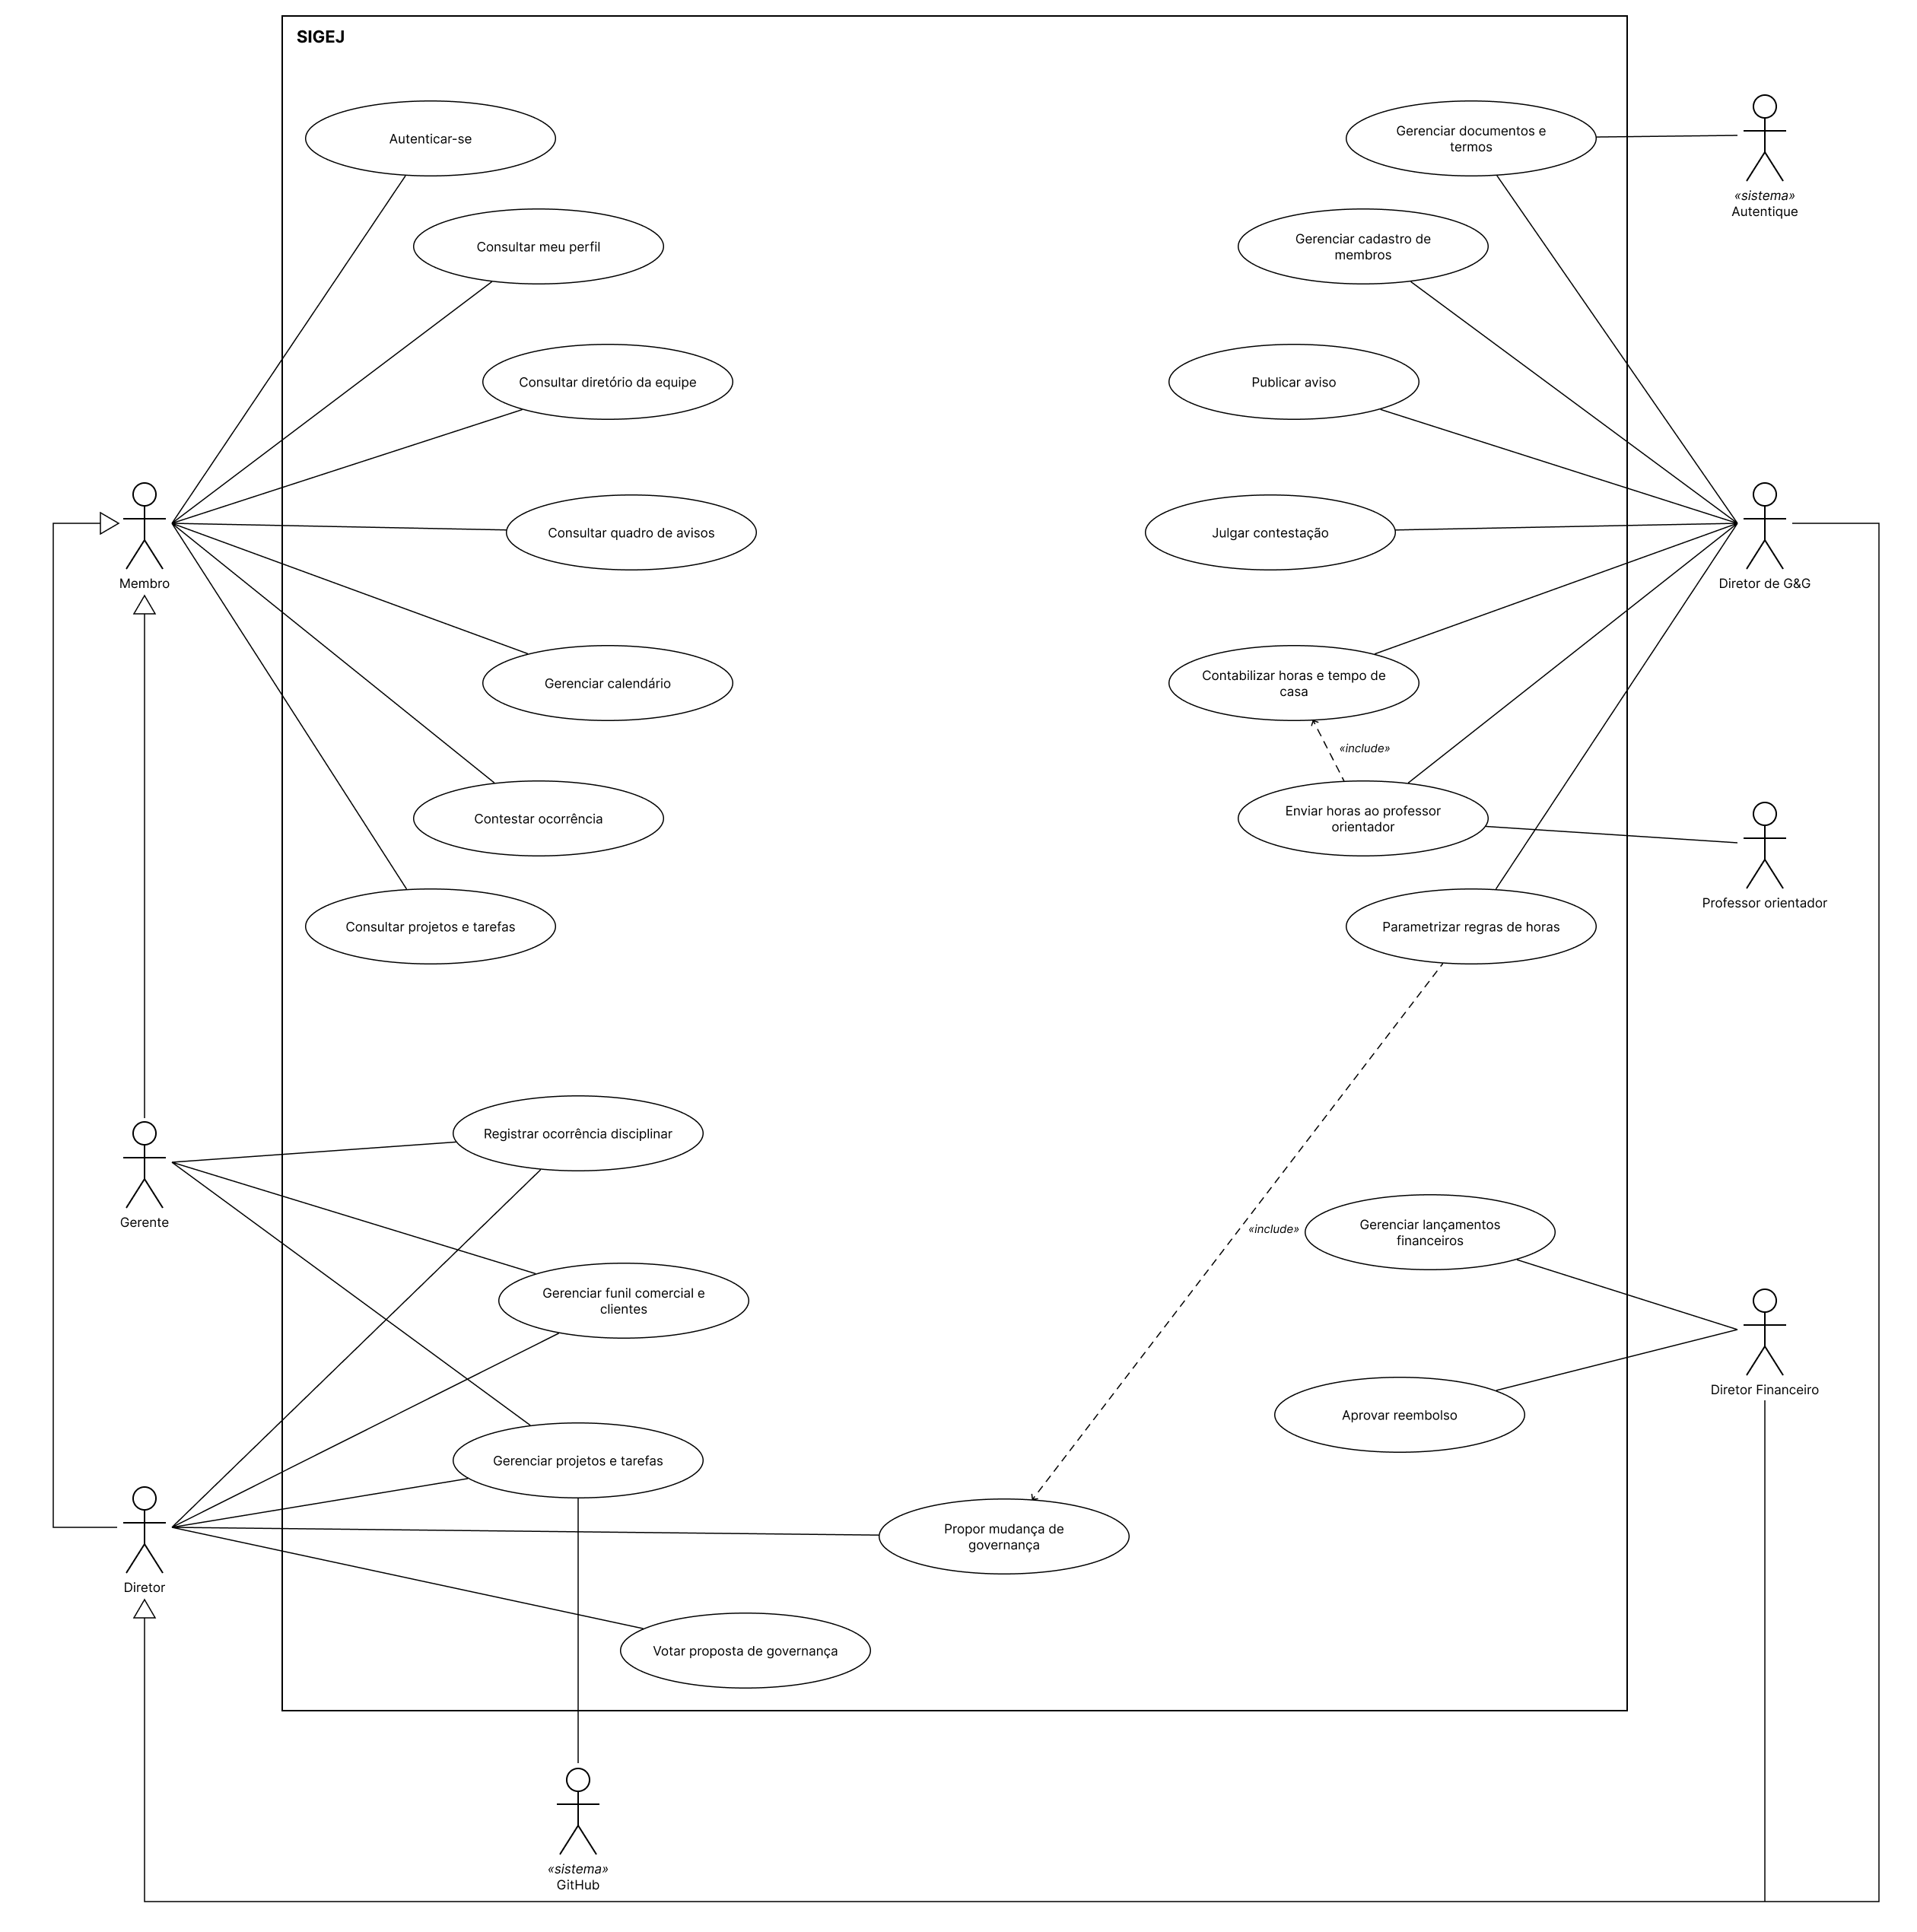
\includegraphics[width=0.9\textwidth,height=0.7\textheight,keepaspectratio]{diagrama.png}
    \label{fig:dcu-commit}
\end{figure}

% Bloqueia estritamente a descida da imagem para as seções abaixo
\clearpage

\subsection{Regras do negócio}

\textbf{RN01 - Unicidade Cadastral}: Todo integrante deve possuir identificação única no banco de dados referenciada por seu CPF e número de matrícula acadêmica.

\textbf{RN02 - Cômputo Proporcional de Horas}: As horas de extensão são computadas diretamente multiplicando o intervalo de tempo de permanência no cargo pela taxa horária previamente homologada para a função.

\textbf{RN03 - Preservação Histórica e Desativação Lógica}: Membros vinculados a horas, pontos, termos ou eventos institucionais não sofrem exclusão física; sua inativação deve ser efetuada via alteração para status ``Desligado'' ou ``Alumnus''.

\textbf{RN04 - Visibilidade Restrita a Membros Ativos}: O diretório geral de consulta corporativa deve exibir somente os integrantes com vínculo ativo, ficando os registros históricos restritos à consulta das diretorias de Gestão de Pessoas e Jurídico.

\textbf{RN05 - Caducidade e Agravamento de Penalidades}: Toda ocorrência disciplinar possui data de validade definida no ato de lançamento; reincidências ocorridas dentro do prazo de vigência acarretam a incidência do multiplicador agravante automático.

\textbf{RN06 - Incompatibilidade de Agendamentos}: O sistema deve impedir a confirmação de reuniões individuais caso um dos participantes conste como confirmado em outro compromisso formal ou Reunião Geral no mesmo horário.

\subsection{Descrição dos Casos de Uso}

\begin{casodeuso}
\textbf{UC-01 - Login e Autenticação}

\textbf{Sumário:} Usuário informa suas credenciais para autenticar-se na plataforma.

\textbf{Ator Primário:} Membro, Líder de Área, Jurídico ou Administrador.

\textbf{Pré-condições:} Usuário previamente cadastrado e com status ativo no banco de dados.

\textbf{Fluxo Principal}

\noindent 1. Usuário acessa o sistema web.\\
2. Usuário fornece e-mail institucional e senha de acesso.\\
3. Sistema valida as credenciais contra a base autenticada.\\
4. Sistema inicia a sessão do usuário e direciona para o painel de seu perfil.

\textbf{Fluxo de Exceção (1):} Credenciais Inválidas
\begin{itemize}
    \item a. Sistema informa divergência de credenciais e convida o usuário a repetir a tentativa.
\end{itemize}

\textbf{Pós-condições:} Usuário autenticado na aplicação com perfil e níveis de acesso carregados.
\end{casodeuso}

\begin{casodeuso}
\textbf{UC-02 - Gerenciar Cadastro de Membros}

\textbf{Sumário:} Administrador executa operações de cadastro, consulta, edição e desativação de integrantes da empresa.

\textbf{Ator Primário:} Administrador / Gestão de Pessoas.

\textbf{Pré-condições:} Administrador devidamente autenticado.

\textbf{Fluxo Principal}

\noindent 1. Administrador acessa o módulo de Gestão de Membros.\\
2. Sistema lista os membros cadastrados com suporte a filtros por diretoria, campus e status.\\
3. Administrador aciona o formulário de inclusão e preenche os campos: matrícula, CPF, RG, nome completo, curso, campus, endereço, e-mail institucional, GitHub, diretoria, área/squad, cargo e data de ingresso.\\
4. Sistema valida a unicidade cadastral (conforme RN01) e persiste o novo registro.\\
5. Para membros já existentes, o administrador pode atualizar informações ou alterar o status para ``Desligado'' ou ``Alumnus''.\\
6. Sistema armazena as alterações mantendo a integridade histórica.

\textbf{Fluxo de Exceção (1):} Violação de Unicidade Cadastral (RN01)
\begin{itemize}
    \item a. Sistema acusa documento já existente no banco de dados e interrompe o cadastro.
\end{itemize}

\textbf{Fluxo de Exceção (2):} Tentativa de Exclusão Física com Vínculos (RN03)
\begin{itemize}
    \item a. Sistema impede a exclusão física caso haja dependências em horas ou pontos e orienta a inativação lógica.
\end{itemize}

\textbf{Pós-condições:} Membro registrado ou atualizado na base corporativa.
\end{casodeuso}

\begin{casodeuso}
\textbf{UC-06 - Notificar e Enviar Horas para a Coordenação}

\textbf{Sumário:} Sistema gera o lote de horas apuradas e encaminha demonstrativo oficial por e-mail à coordenação do curso.

\textbf{Ator Primário:} Administrador / Gestão de Pessoas.

\textbf{Atores Secundários:} Servidor SMTP de E-mail Institucional.

\textbf{Pré-condições:} Membros selecionados com horas de extensão calculadas e conferidas.

\textbf{Fluxo Principal}

\noindent 1. Administrador seleciona o período e solicita a apuração das horas de extensão.\\
2. Sistema exibe a tabela com matrícula, nome, curso, campus e somatório de horas.\\
3. Administrador confirma o encerramento do lote e solicita o disparo à coordenação.\\
4. Sistema anexa o relatório formal e envia a notificação via e-mail ao endereço do coordenador acadêmico.\\
5. Sistema atualiza o status das horas para ``Enviado''.

\textbf{Pós-condições:} Demonstrativo de horas enviado à coordenação acadêmica para validação no SIGAA.
\end{casodeuso}

\begin{casodeuso}
\textbf{UC-07 - Gerenciar Pontos e Penalidades}

\textbf{Sumário:} Líderes registram penalidades disciplinares e acompanham o status de expiração e agravantes.

\textbf{Ator Primário:} Administrador / Gestão de Pessoas ou Líder de Área.

\textbf{Pré-condições:} Usuário autenticado com perfil de liderança.

\textbf{Fluxo Principal}

\noindent 1. Usuário abre a tela de registro de ocorrência disciplinar.\\
2. Usuário seleciona o membro, digita a infração, os pontos correspondentes e anexa a justificativa.\\
3. Sistema confere o histórico e calcula automaticamente o multiplicador de reincidência e a data limite de expiração (conforme RN05).\\
4. Usuário revisa e confirma o lançamento.\\
5. Sistema persiste a advertência e ajusta o saldo disciplinar ativo do membro.

\textbf{Pós-condições:} Ocorrência disciplinar registrada com cômputo de expiração programado.
\end{casodeuso}

\section{Requisitos Não-Funcionais (RNF)}

\textbf{RNF01 - Portabilidade Web}\\
\textbf{Categoria:} Portabilidade\\
\textbf{Prioridade:} Essencial\\
O sistema deve executar de forma compatível nos principais navegadores modernos (Google Chrome, Mozilla Firefox, Safari, Microsoft Edge) em plataformas desktop e mobile.

\textbf{RNF02 - Desempenho e Tempo de Resposta}\\
\textbf{Categoria:} Desempenho\\
\textbf{Prioridade:} Importante\\
As telas com listagens de membros, pontuações e relatórios de horas devem concluir o carregamento em tempo não superior a 2 segundos sob conexão convencional.

\textbf{RNF03 - Controle de Acesso e Permissões (RBAC)}\\
\textbf{Categoria:} Segurança\\
\textbf{Prioridade:} Essencial\\
O sistema deve implementar autenticação baseada em perfis de acesso, restringindo a visualização de documentos civis e dados disciplinares apenas a gestores e ao setor Jurídico.

\textbf{RNF04 - Criptografia de Dados}\\
\textbf{Categoria:} Segurança\\
\textbf{Prioridade:} Essencial\\
Senhas de acesso devem ser protegidas por algoritmos de hash com salgamento seguro (BCrypt/Argon2) e campos de documentos civis sensíveis devem trafegar e repousar sob criptografia.

\textbf{RNF05 - Responsividade e Usabilidade}\\
\textbf{Categoria:} Facilidade de uso\\
\textbf{Prioridade:} Essencial\\
A interface gráfica de usuário deve ser responsiva, adaptando-se sem quebra de leiaute a diferentes resoluções de notebooks, computadores e smartphones.

\textbf{RNF06 - Trilha de Auditoria (Logs)}\\
\textbf{Categoria:} Confiabilidade\\
\textbf{Prioridade:} Importante\\
Todas as rotinas de manipulação, alteração de horas e homologação de penalidades devem gravar logs imutáveis contendo data, hora e identificação do autor da operação.
% ----------------------------------------------------------
% 6. Projeto de Interação
% ----------------------------------------------------------
\chapter{Projeto de Interação}
\label{cap:interacao}

Link para o Projeto de Interação do Sistema no Figma: 

\noindent\url{https://www.figma.com/design/DR6oCNn8QeMXILJPJx4L4D/Sem-t%C3%ADtulo?node-id=0-1&p=f&t=UNW3lNd1nkxwVpfd-0}

Abaixo são apresentados os protótipos das telas de interface com o usuário elaborados no Figma, estruturados em conformidade com as funcionalidades descritas no Diagrama de Casos de Uso e nas especificações funcionais do sistema.

\begin{center}
\begin{tabular}{|p{2.0cm}|p{11.5cm}|}
\hline
\textbf{PT-001} & \textbf{Autenticação e Acesso ao Sistema (UC-01)} \\
\hline
\multicolumn{2}{|c|}{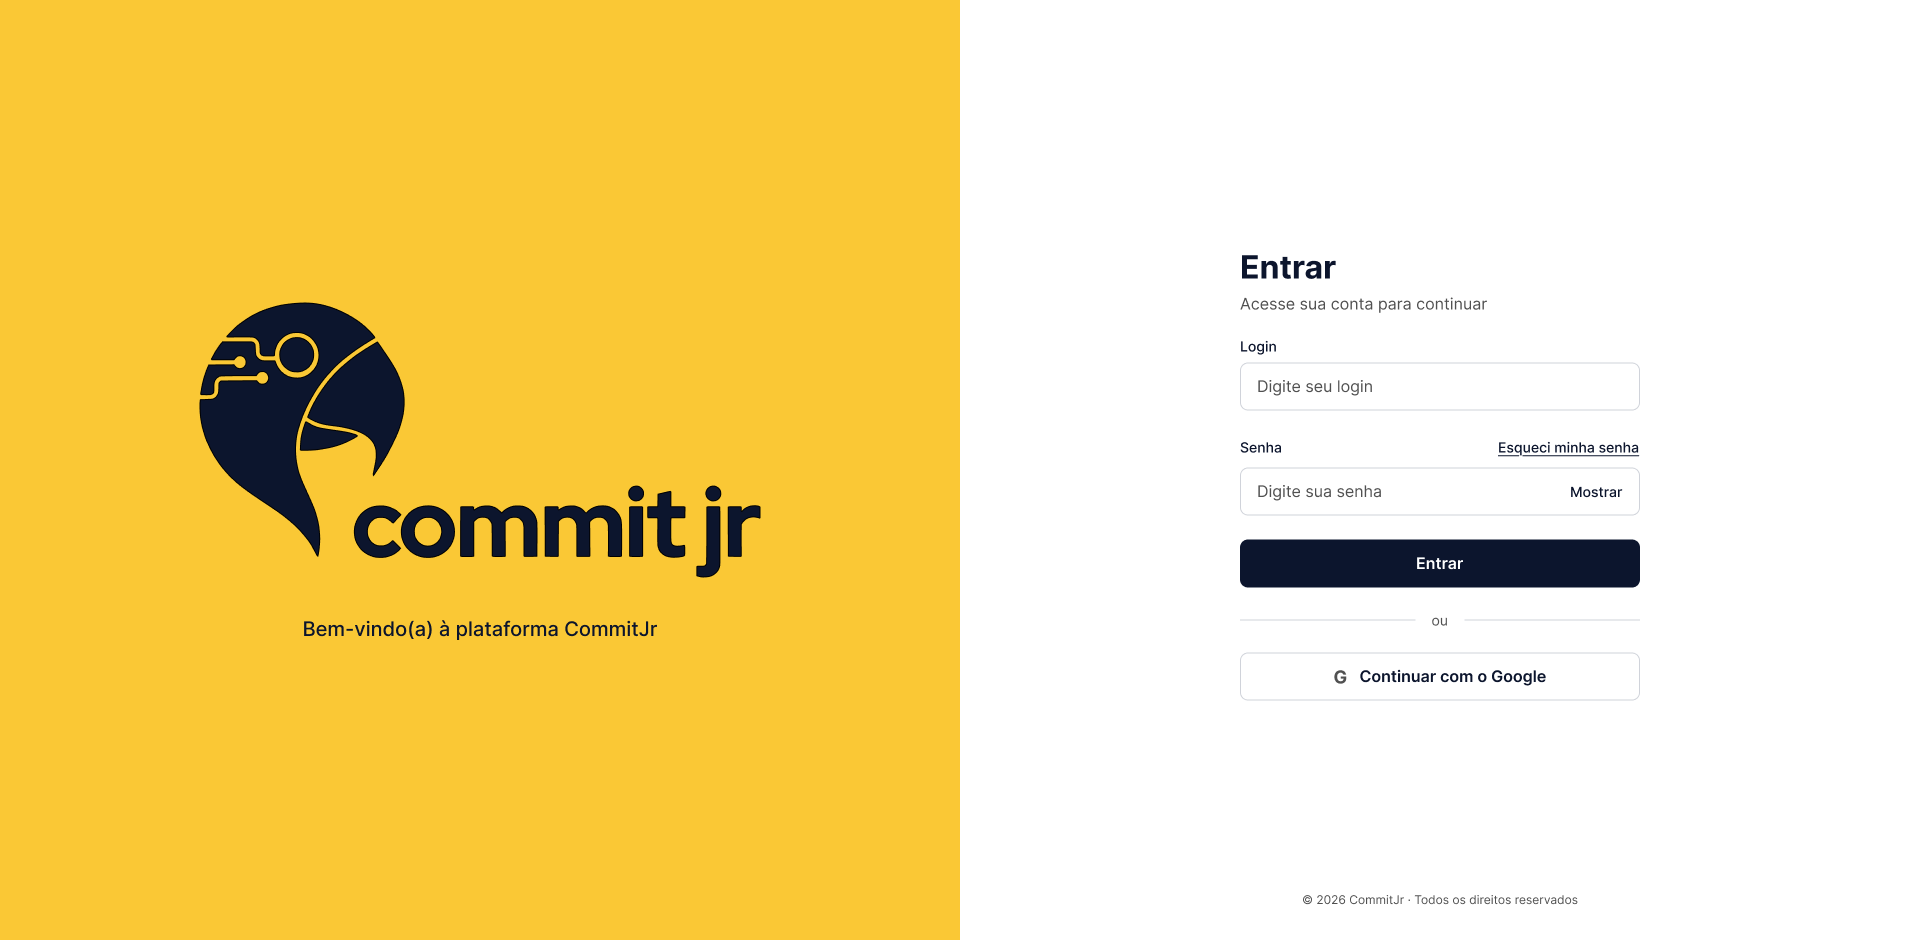
\includegraphics[width=0.88\textwidth]{Telas/login}} \\
\hline
\end{tabular}
\end{center}

\begin{center}
\begin{tabular}{|p{2.0cm}|p{11.5cm}|}
\hline
\textbf{PT-002} & \textbf{Painel Inicial e Dashboard Geral} \\
\hline
\multicolumn{2}{|c|}{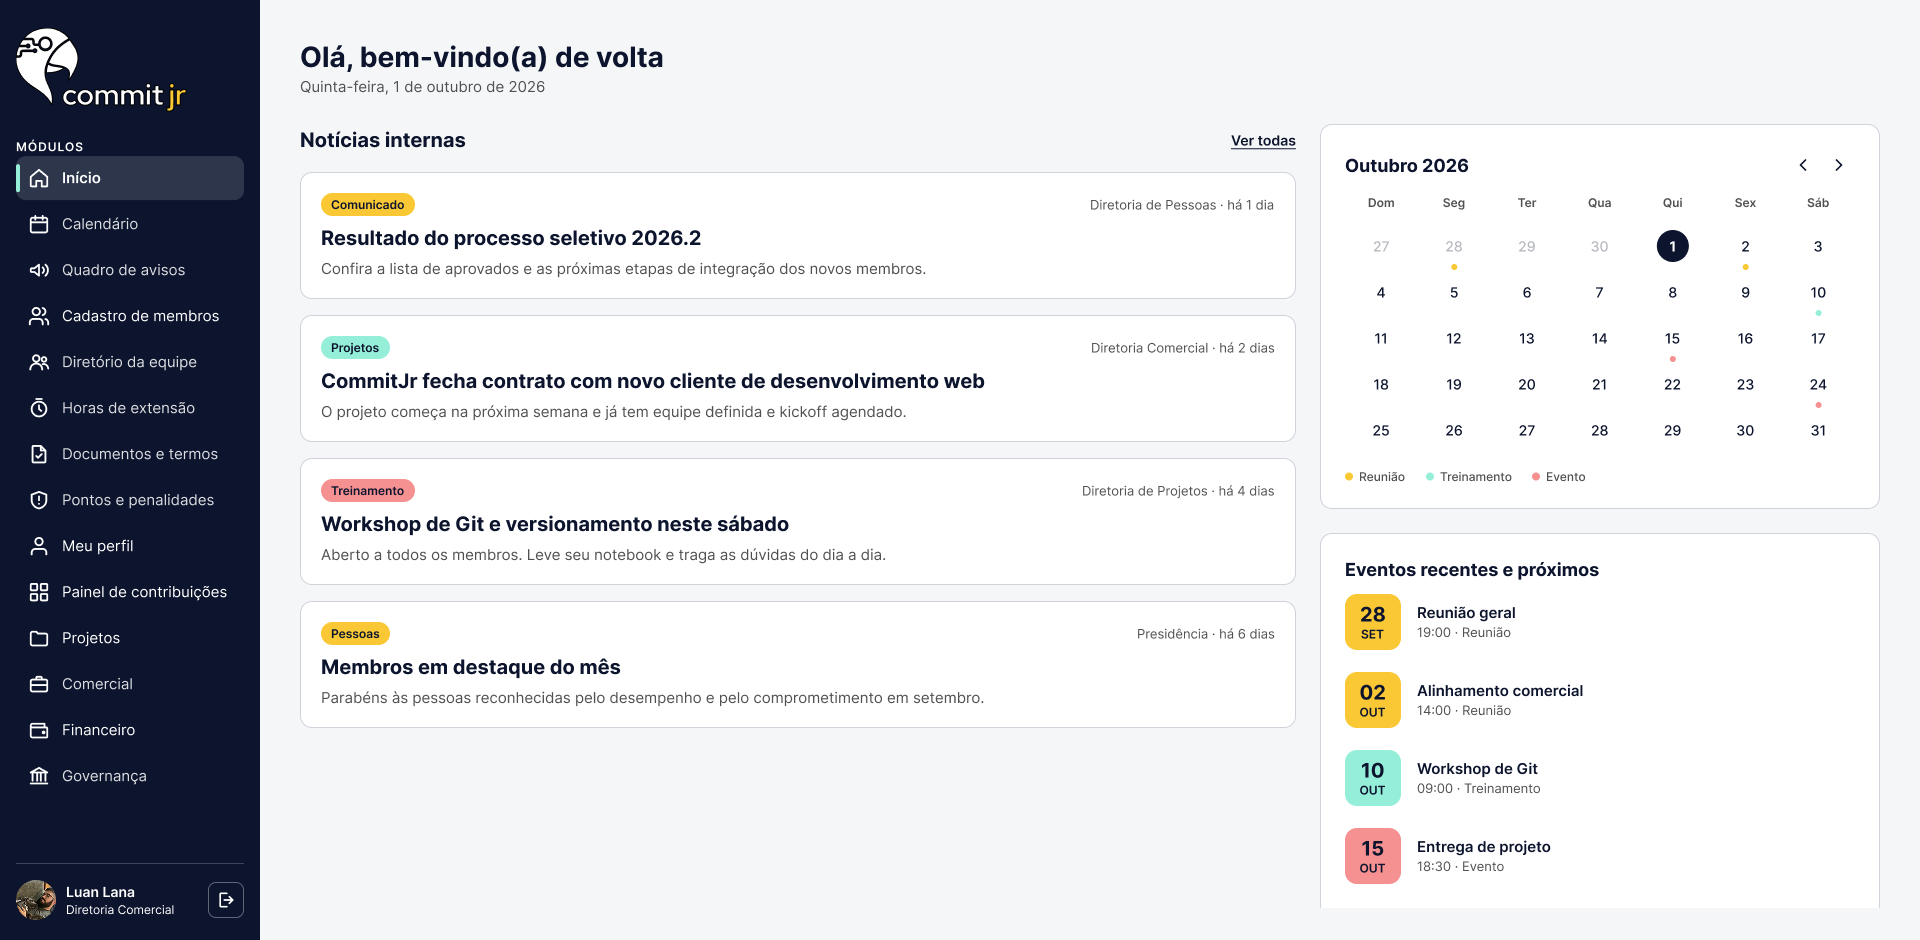
\includegraphics[width=0.88\textwidth]{Telas/inicio}} \\
\hline
\end{tabular}
\end{center}

\begin{center}
\begin{tabular}{|p{2.0cm}|p{11.5cm}|}
\hline
\textbf{PT-003} & \textbf{Meu Perfil de Membro} \\
\hline
\multicolumn{2}{|c|}{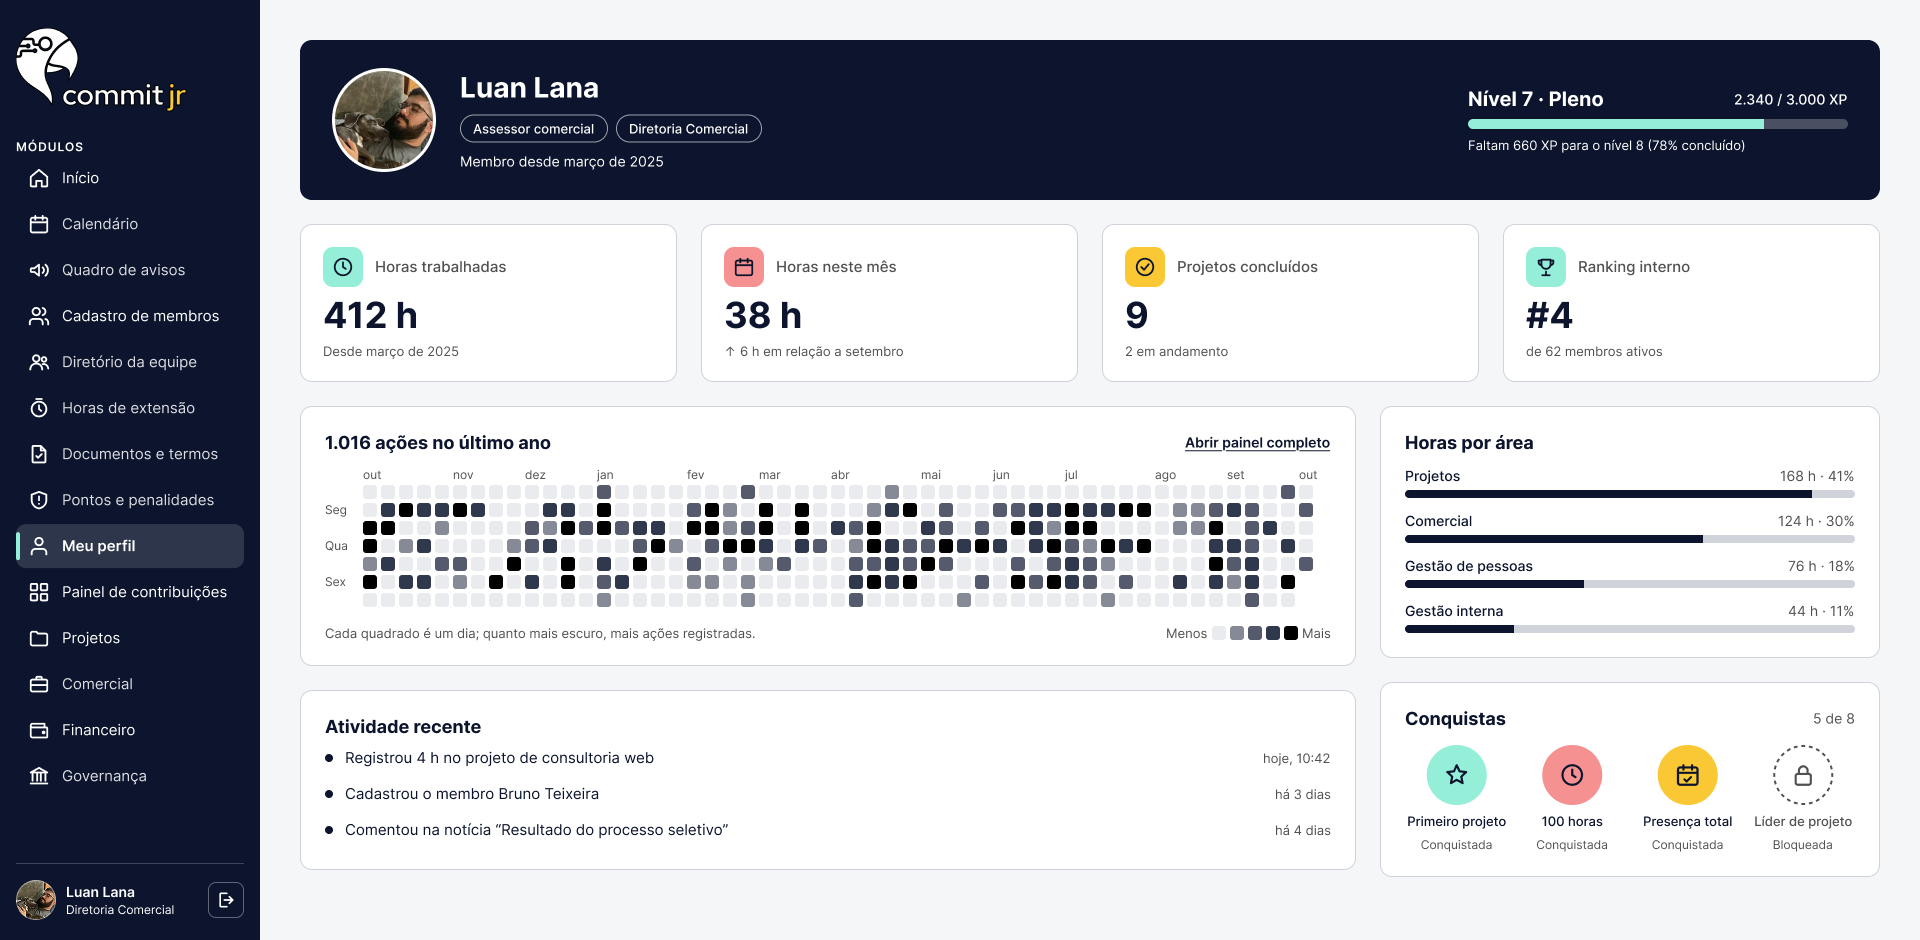
\includegraphics[width=0.88\textwidth]{Telas/meu-perfil}} \\
\hline
\end{tabular}
\end{center}

\begin{center}
\begin{tabular}{|p{2.0cm}|p{11.5cm}|}
\hline
\textbf{PT-004} & \textbf{Cadastro de Membros - Listagem Geral (UC-02)} \\
\hline
\multicolumn{2}{|c|}{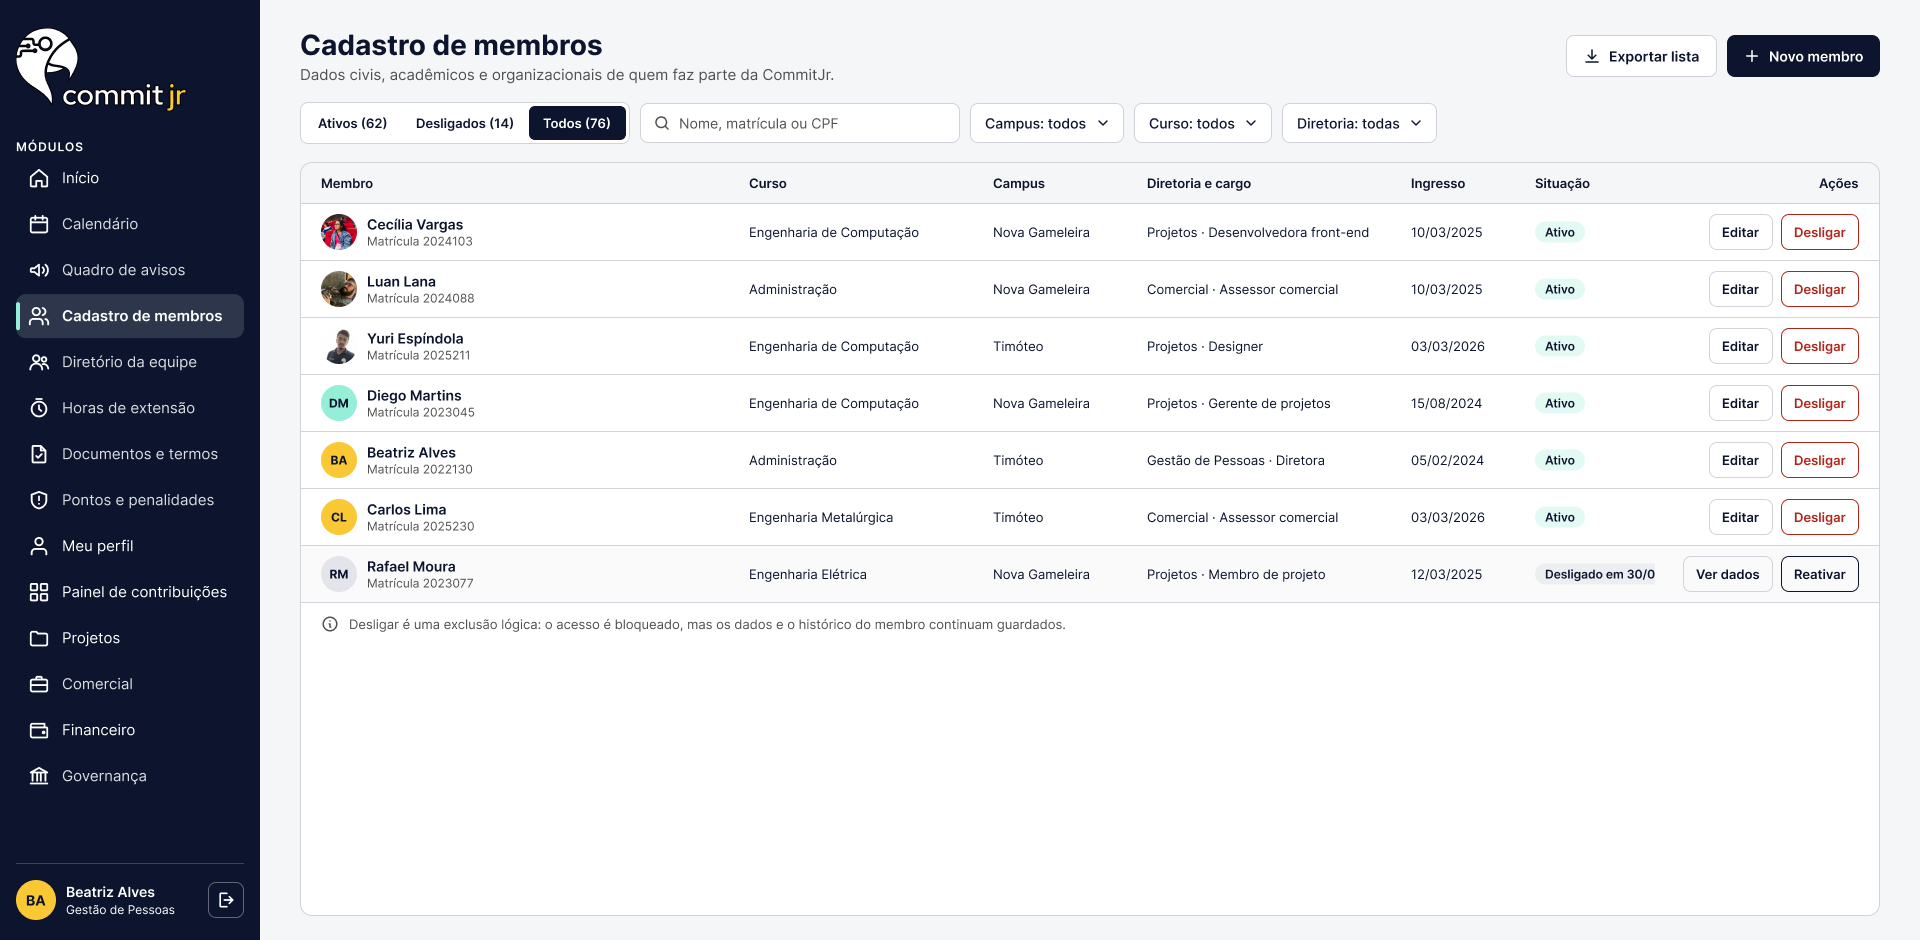
\includegraphics[width=0.88\textwidth]{Telas/membros-lista}} \\
\hline
\end{tabular}
\end{center}

\begin{center}
\begin{tabular}{|p{2.0cm}|p{11.5cm}|}
\hline
\textbf{PT-005} & \textbf{Cadastro de Membros - Edição de Dados (UC-02)} \\
\hline
\multicolumn{2}{|c|}{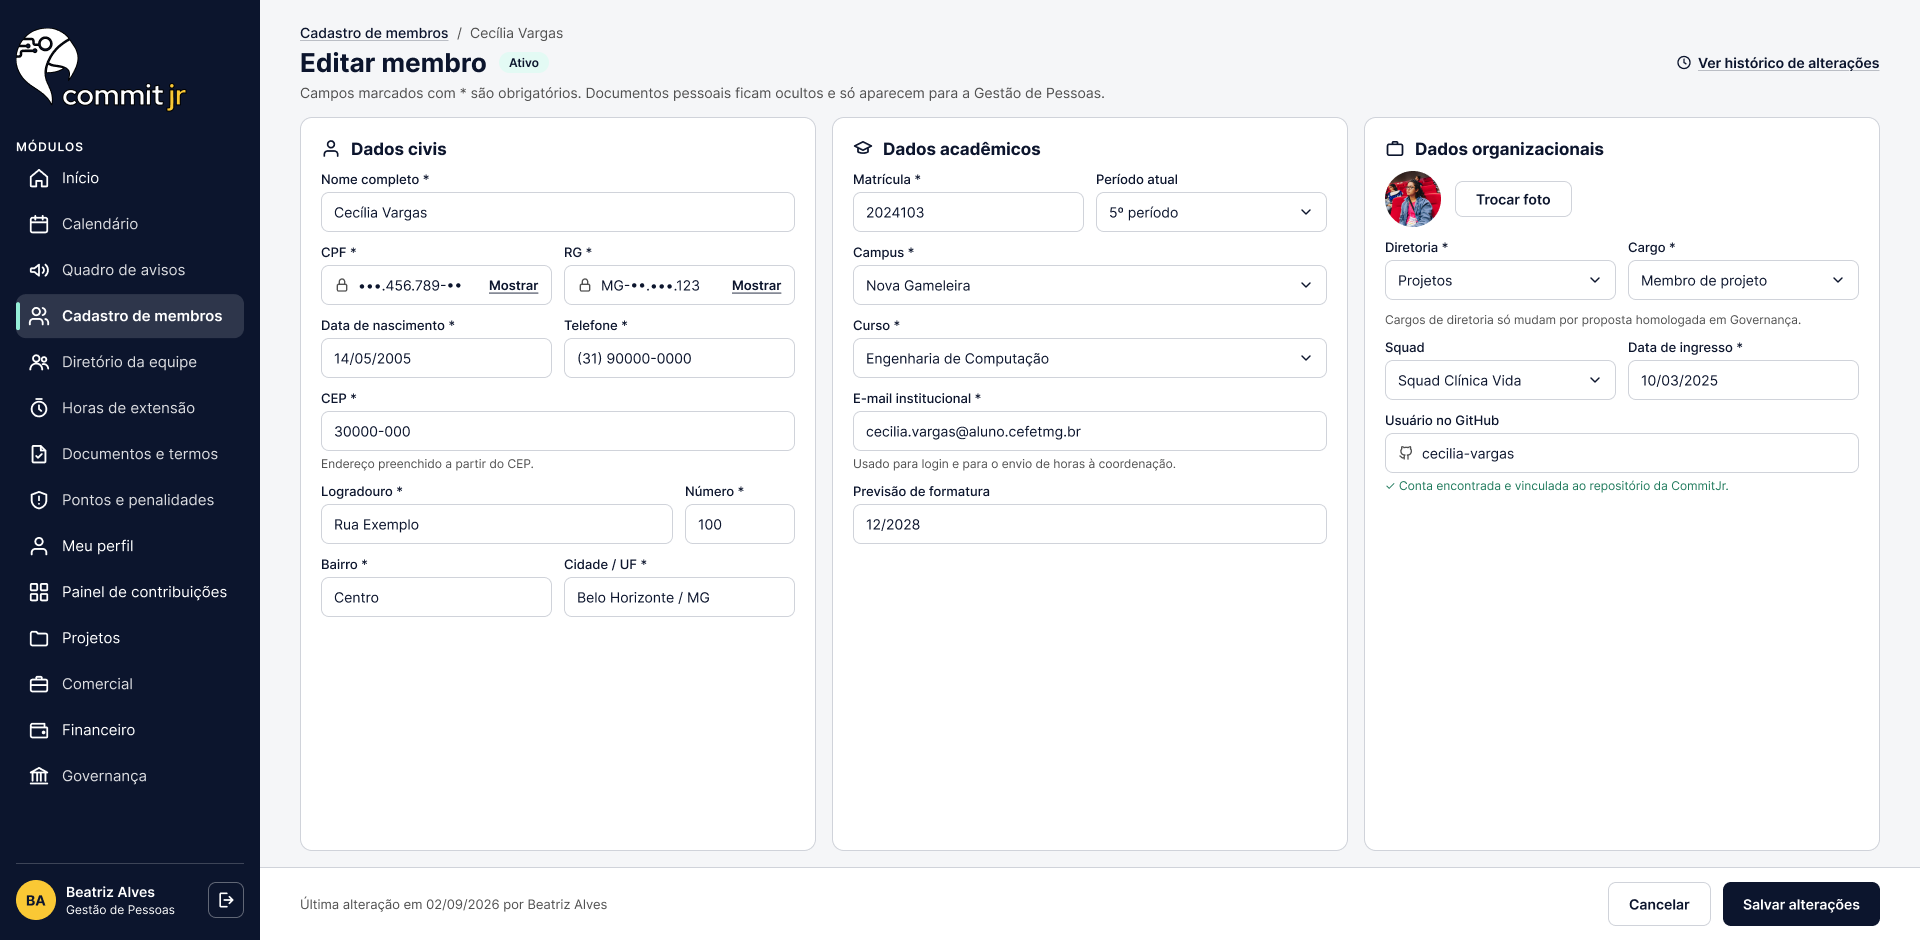
\includegraphics[width=0.88\textwidth]{Telas/membros-editar}} \\
\hline
\end{tabular}
\end{center}

\begin{center}
\begin{tabular}{|p{2.0cm}|p{11.5cm}|}
\hline
\textbf{PT-006} & \textbf{Cadastro de Membros - Desligamento e Inativação Lógica (UC-02)} \\
\hline
\multicolumn{2}{|c|}{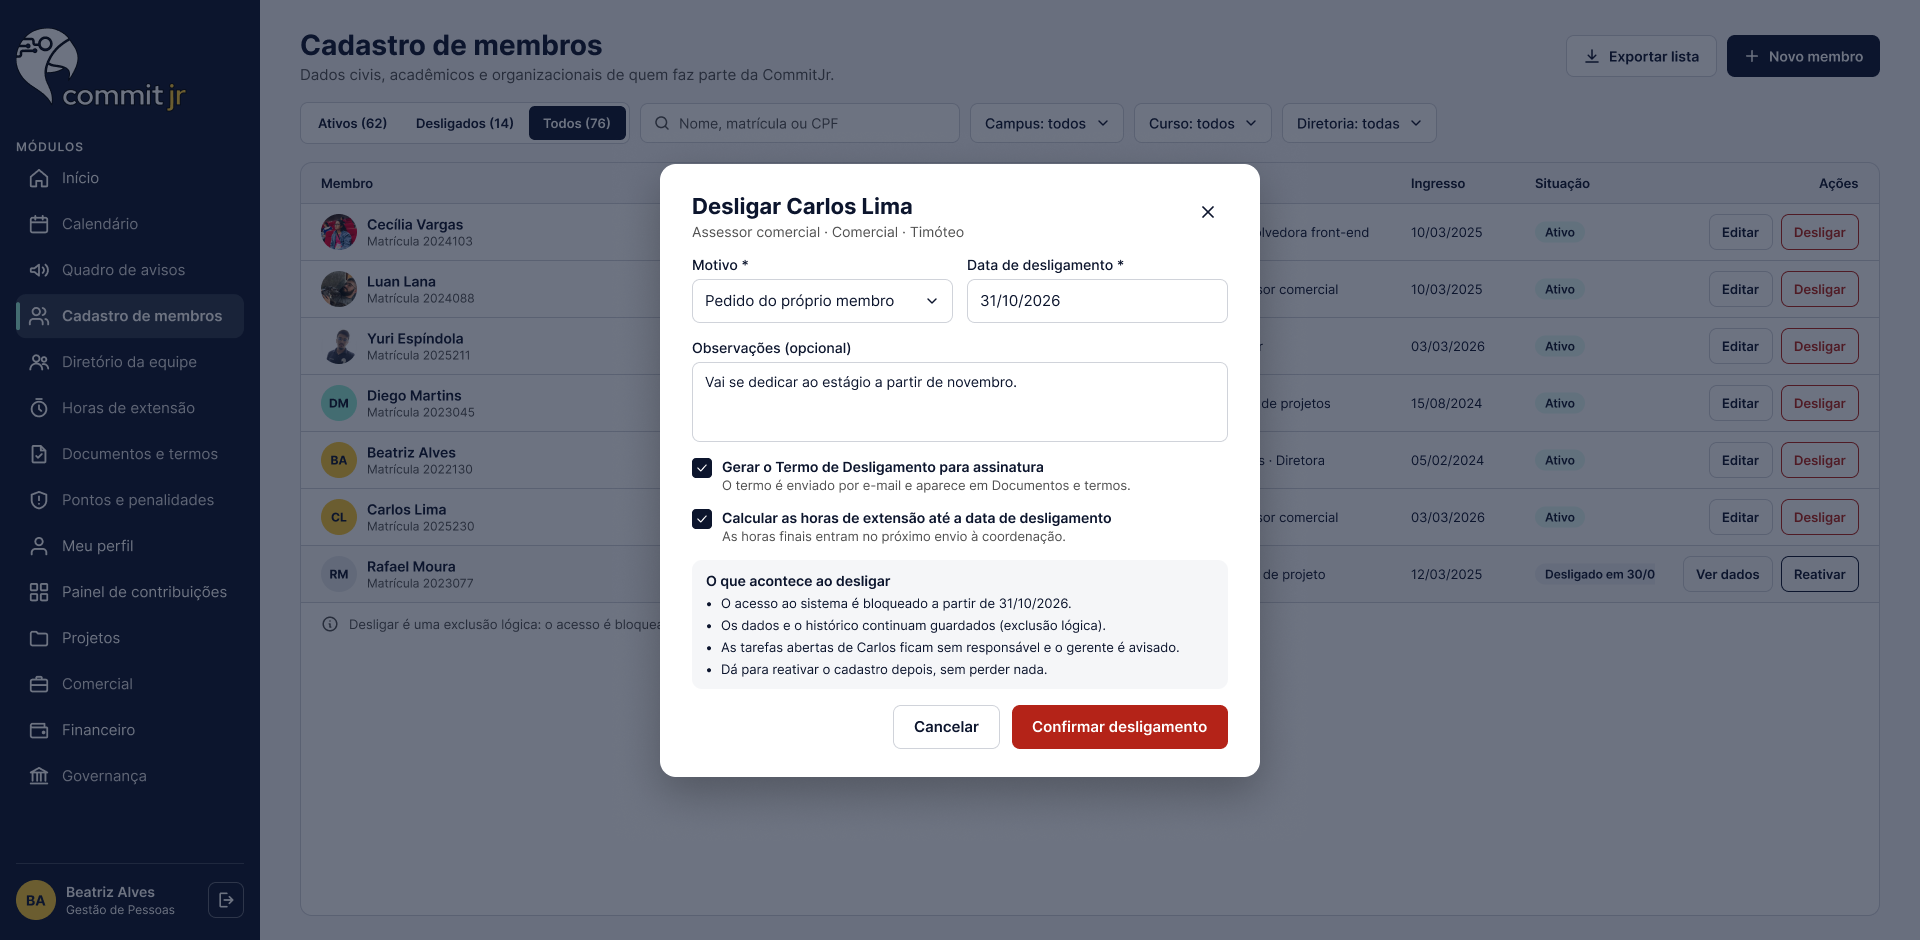
\includegraphics[width=0.88\textwidth]{Telas/membros-desligar}} \\
\hline
\end{tabular}
\end{center}

\begin{center}
\begin{tabular}{|p{2.0cm}|p{11.5cm}|}
\hline
\textbf{PT-007} & \textbf{Diretório Corporativo da Equipe (UC-09)} \\
\hline
\multicolumn{2}{|c|}{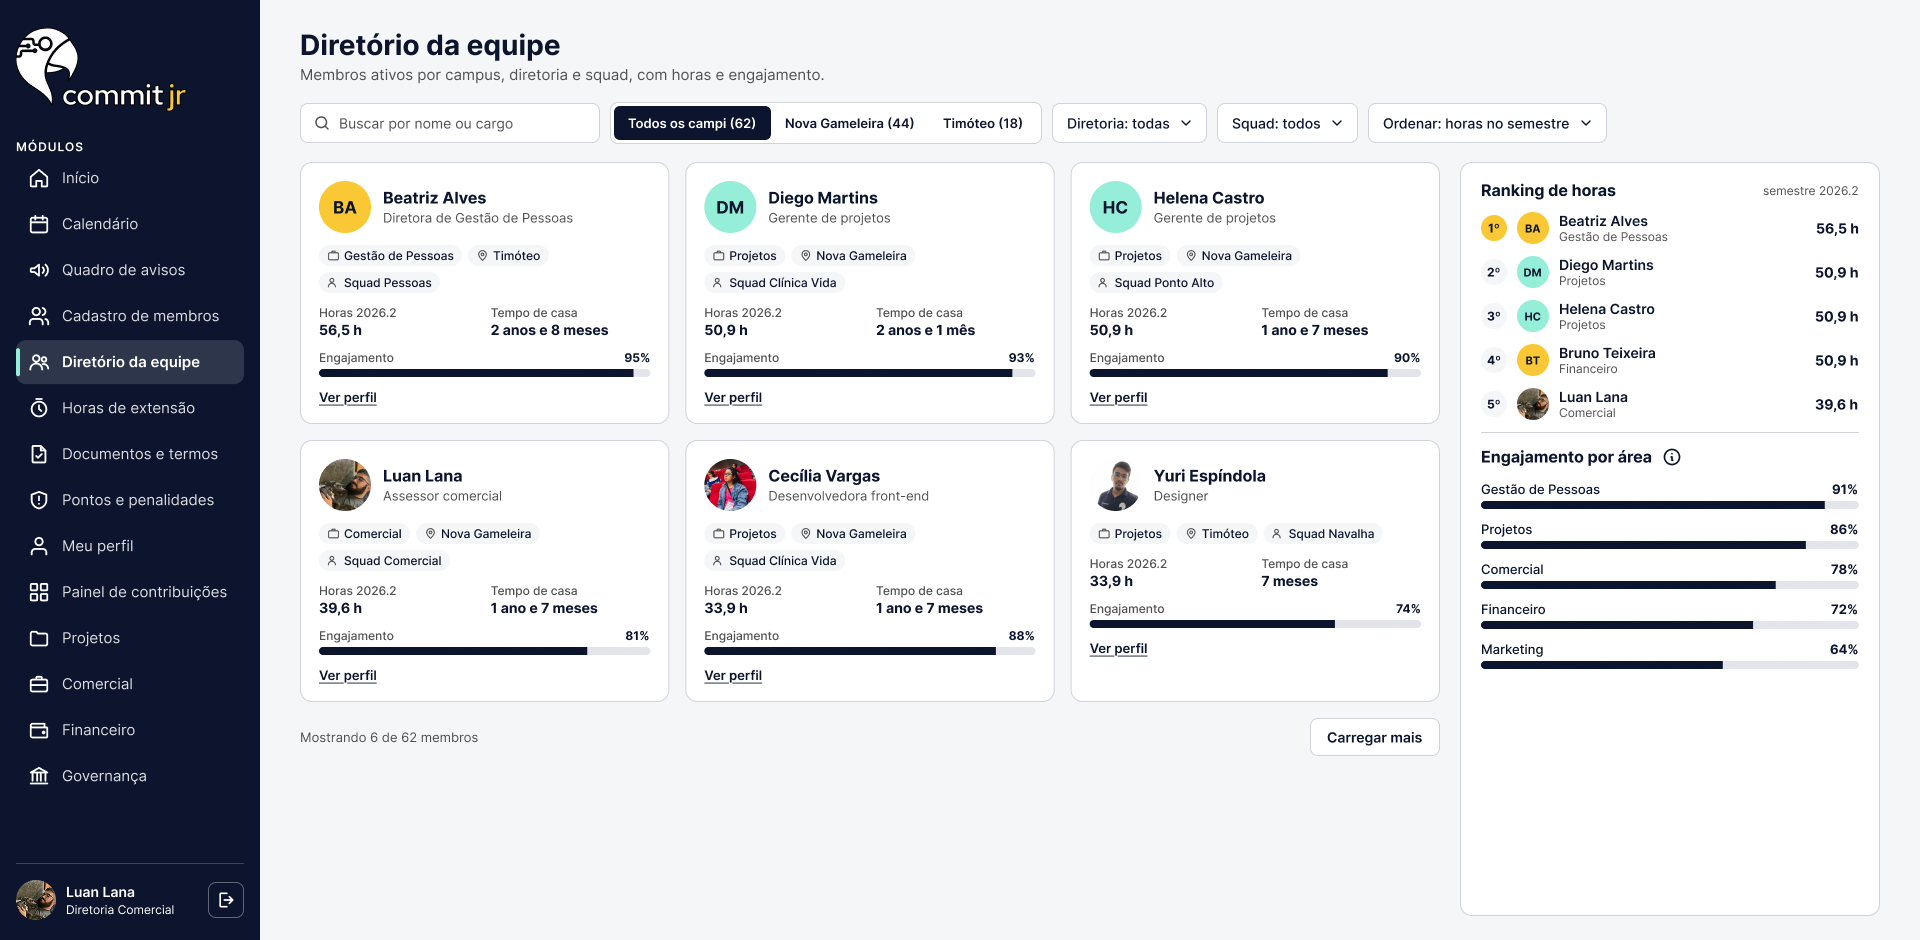
\includegraphics[width=0.88\textwidth]{Telas/diretorio-equipe}} \\
\hline
\end{tabular}
\end{center}

\begin{center}
\begin{tabular}{|p{2.0cm}|p{11.5cm}|}
\hline
\textbf{PT-008} & \textbf{Gestão Documental e Termos Jurídicos (UC-03)} \\
\hline
\multicolumn{2}{|c|}{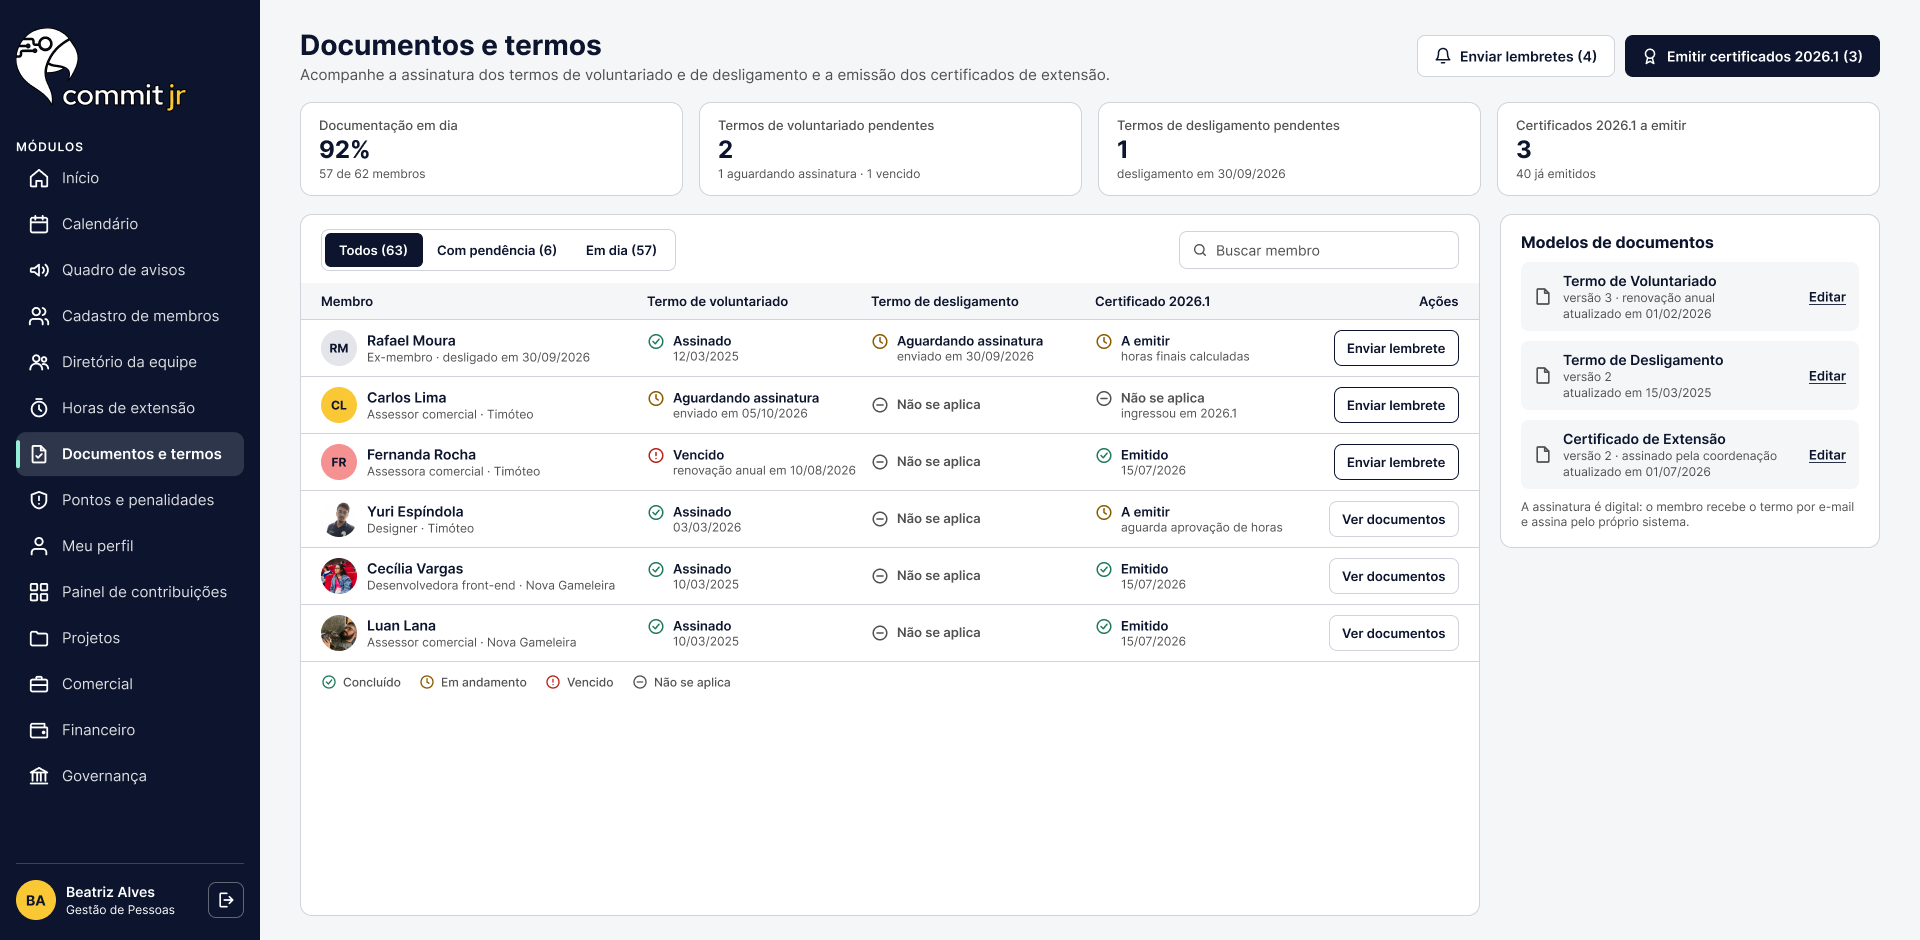
\includegraphics[width=0.88\textwidth]{Telas/documentos-e-termos}} \\
\hline
\end{tabular}
\end{center}

\begin{center}
\begin{tabular}{|p{2.0cm}|p{11.5cm}|}
\hline
\textbf{PT-009} & \textbf{Horas de Extensão - Parametrização por Cargo (UC-04)} \\
\hline
\multicolumn{2}{|c|}{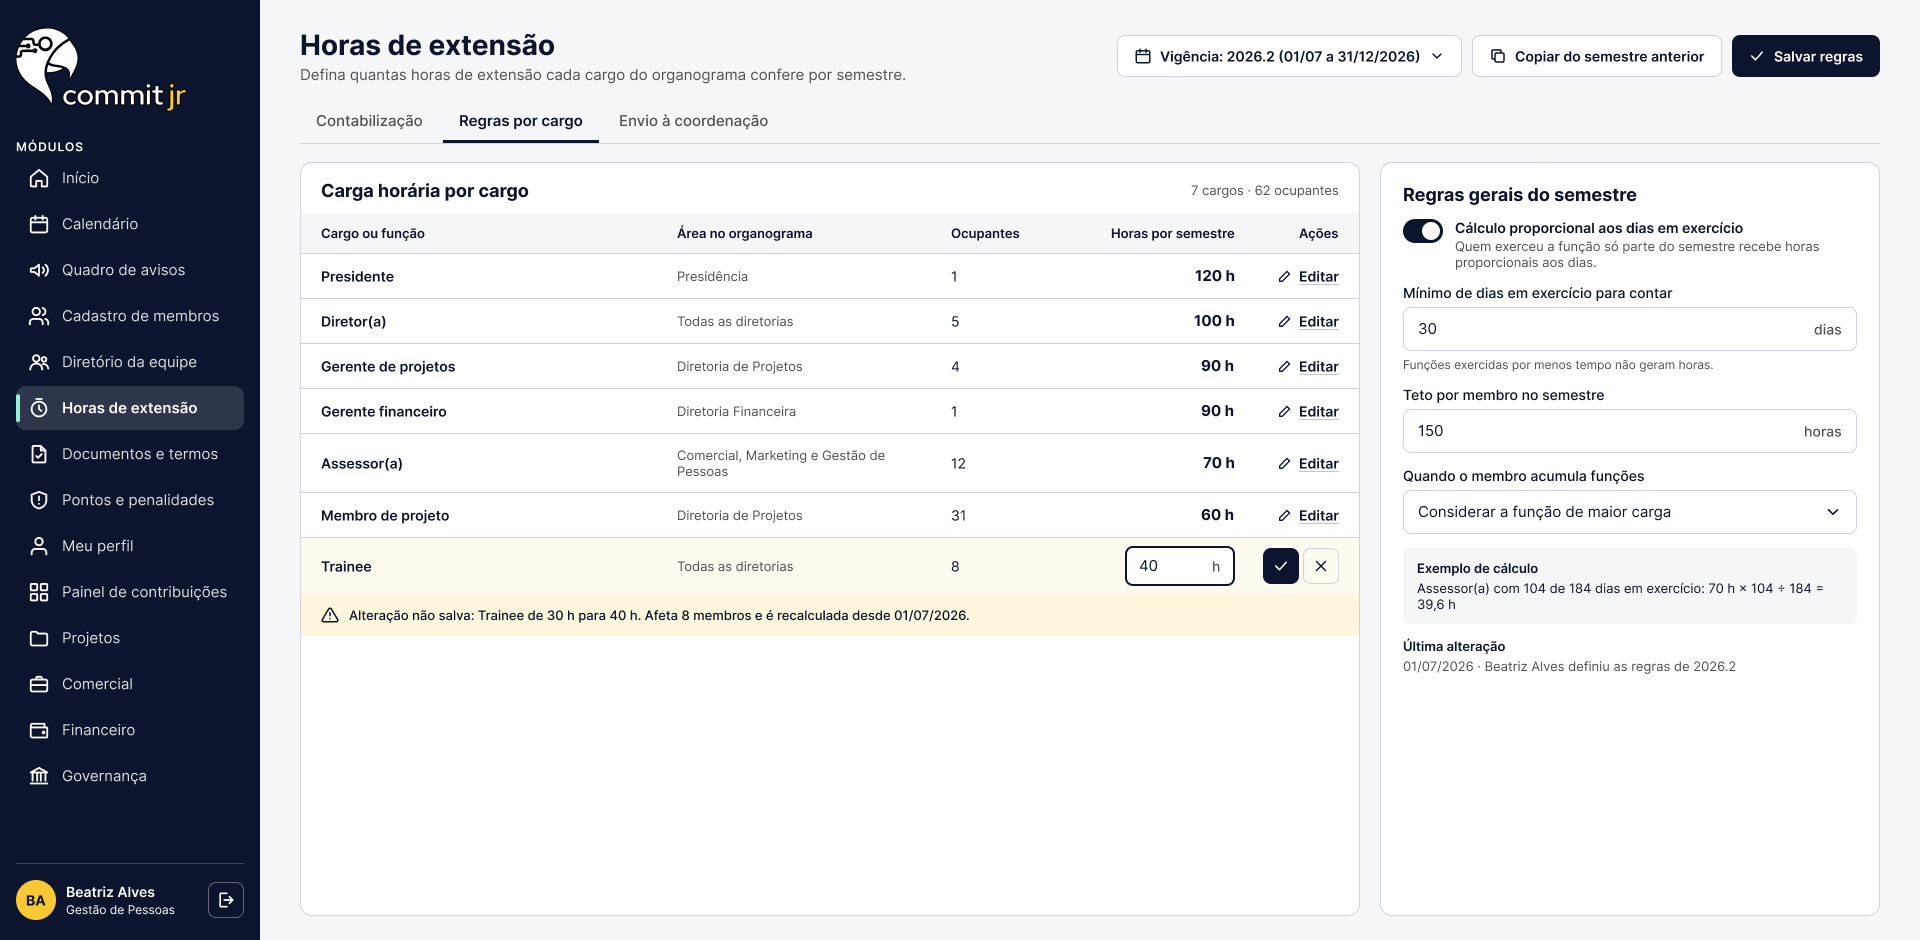
\includegraphics[width=0.88\textwidth]{Telas/horas-regras-por-cargo}} \\
\hline
\end{tabular}
\end{center}

\begin{center}
\begin{tabular}{|p{2.0cm}|p{11.5cm}|}
\hline
\textbf{PT-010} & \textbf{Horas de Extensão - Contabilização Automática (UC-05)} \\
\hline
\multicolumn{2}{|c|}{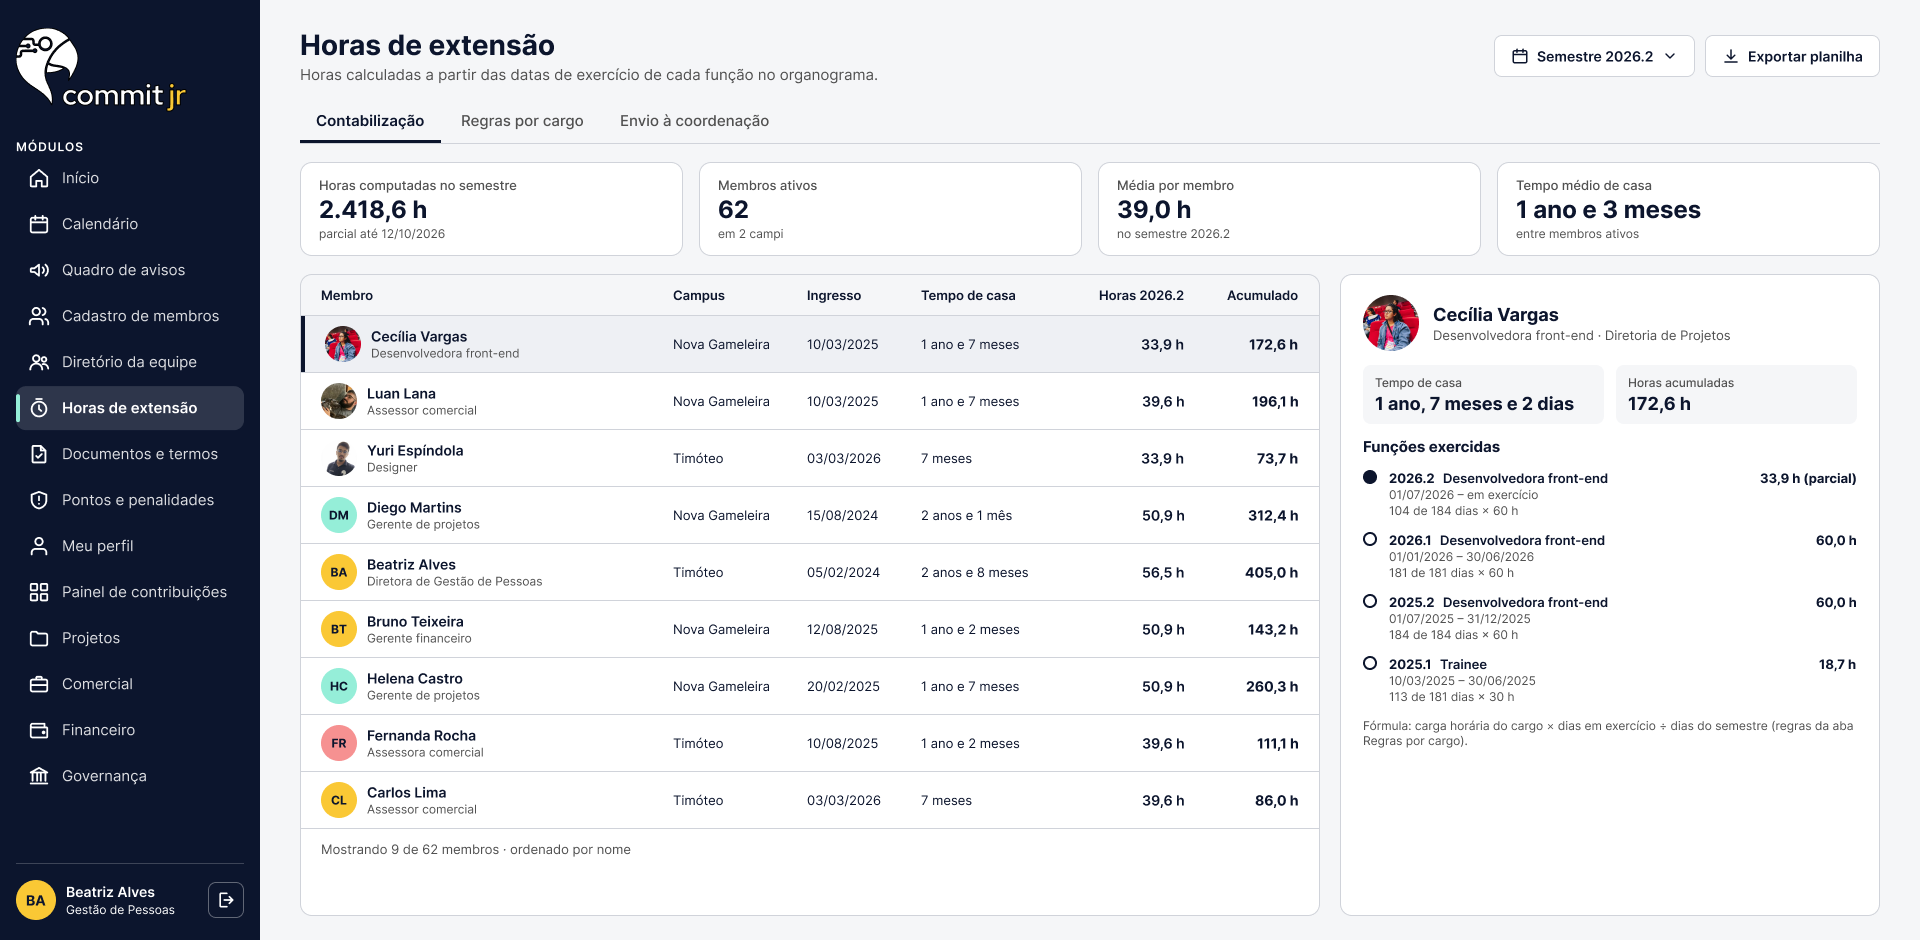
\includegraphics[width=0.88\textwidth]{Telas/horas-contabilizacao}} \\
\hline
\end{tabular}
\end{center}

\begin{center}
\begin{tabular}{|p{2.0cm}|p{11.5cm}|}
\hline
\textbf{PT-011} & \textbf{Horas de Extensão - Envio à Coordenação de Curso (UC-06)} \\
\hline
\multicolumn{2}{|c|}{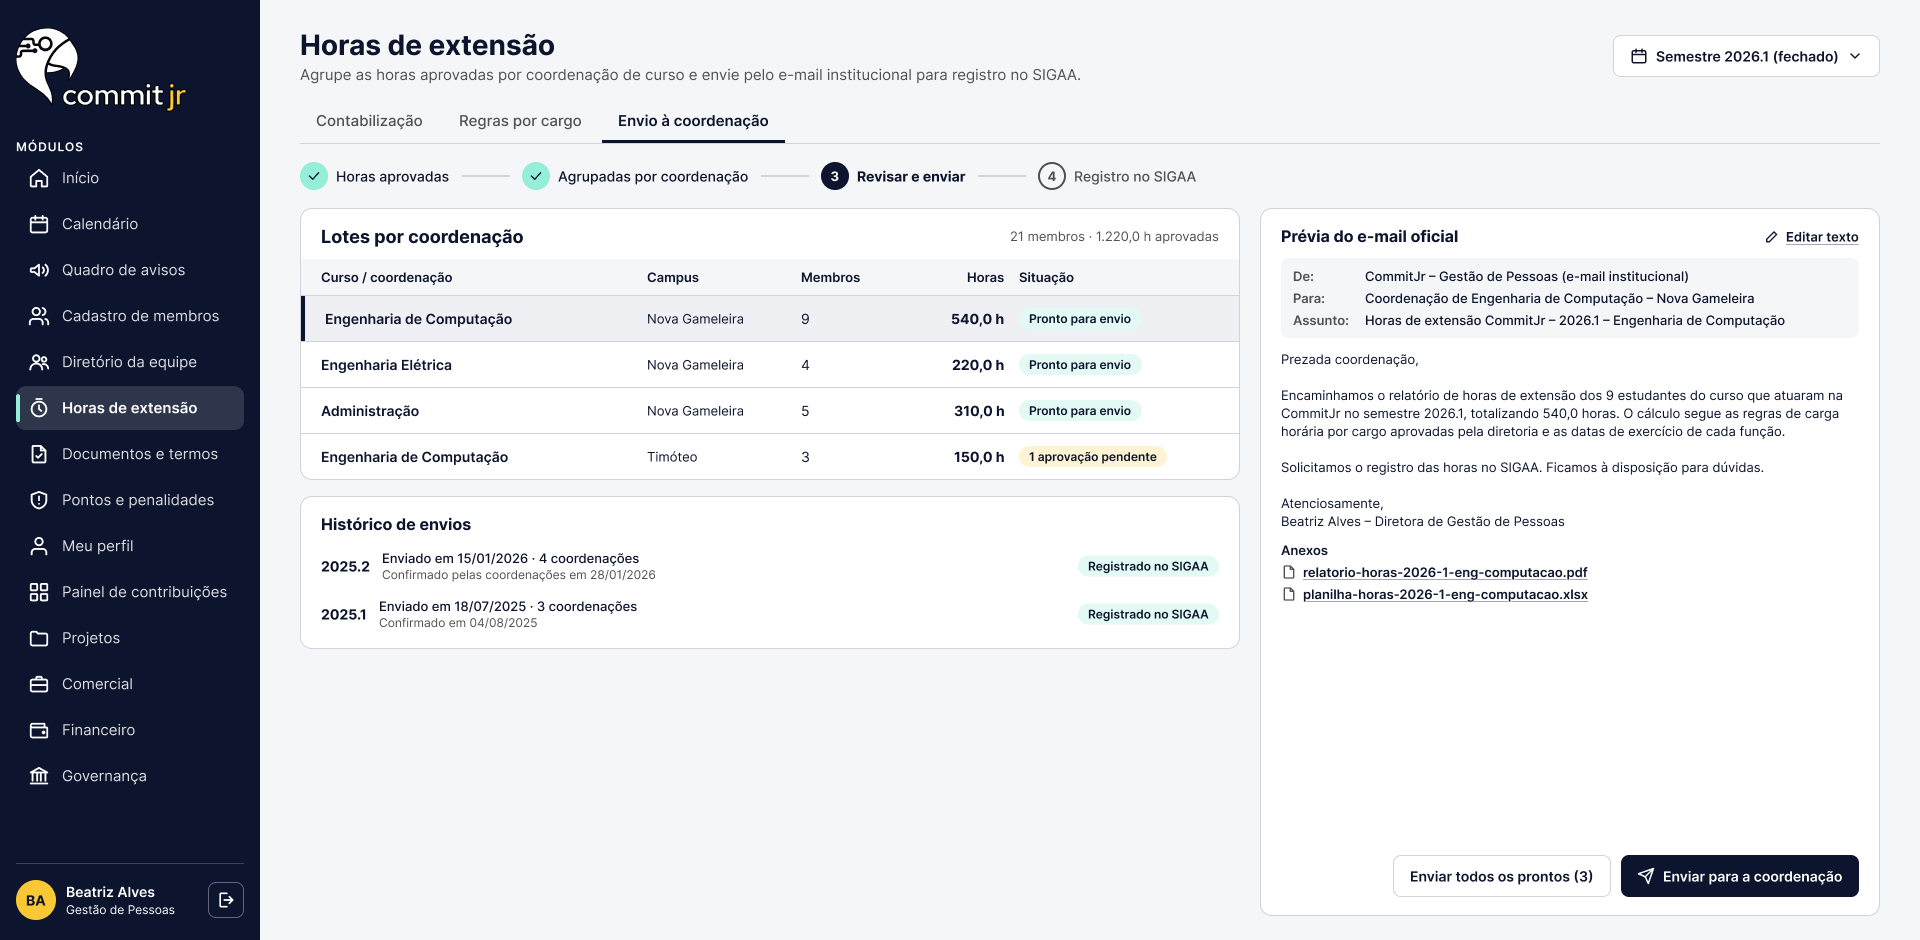
\includegraphics[width=0.88\textwidth]{Telas/horas-envio-coordenacao}} \\
\hline
\end{tabular}
\end{center}

\begin{center}
\begin{tabular}{|p{2.0cm}|p{11.5cm}|}
\hline
\textbf{PT-012} & \textbf{Pontos e Penalidades - Listagem de Membros} \\
\hline
\multicolumn{2}{|c|}{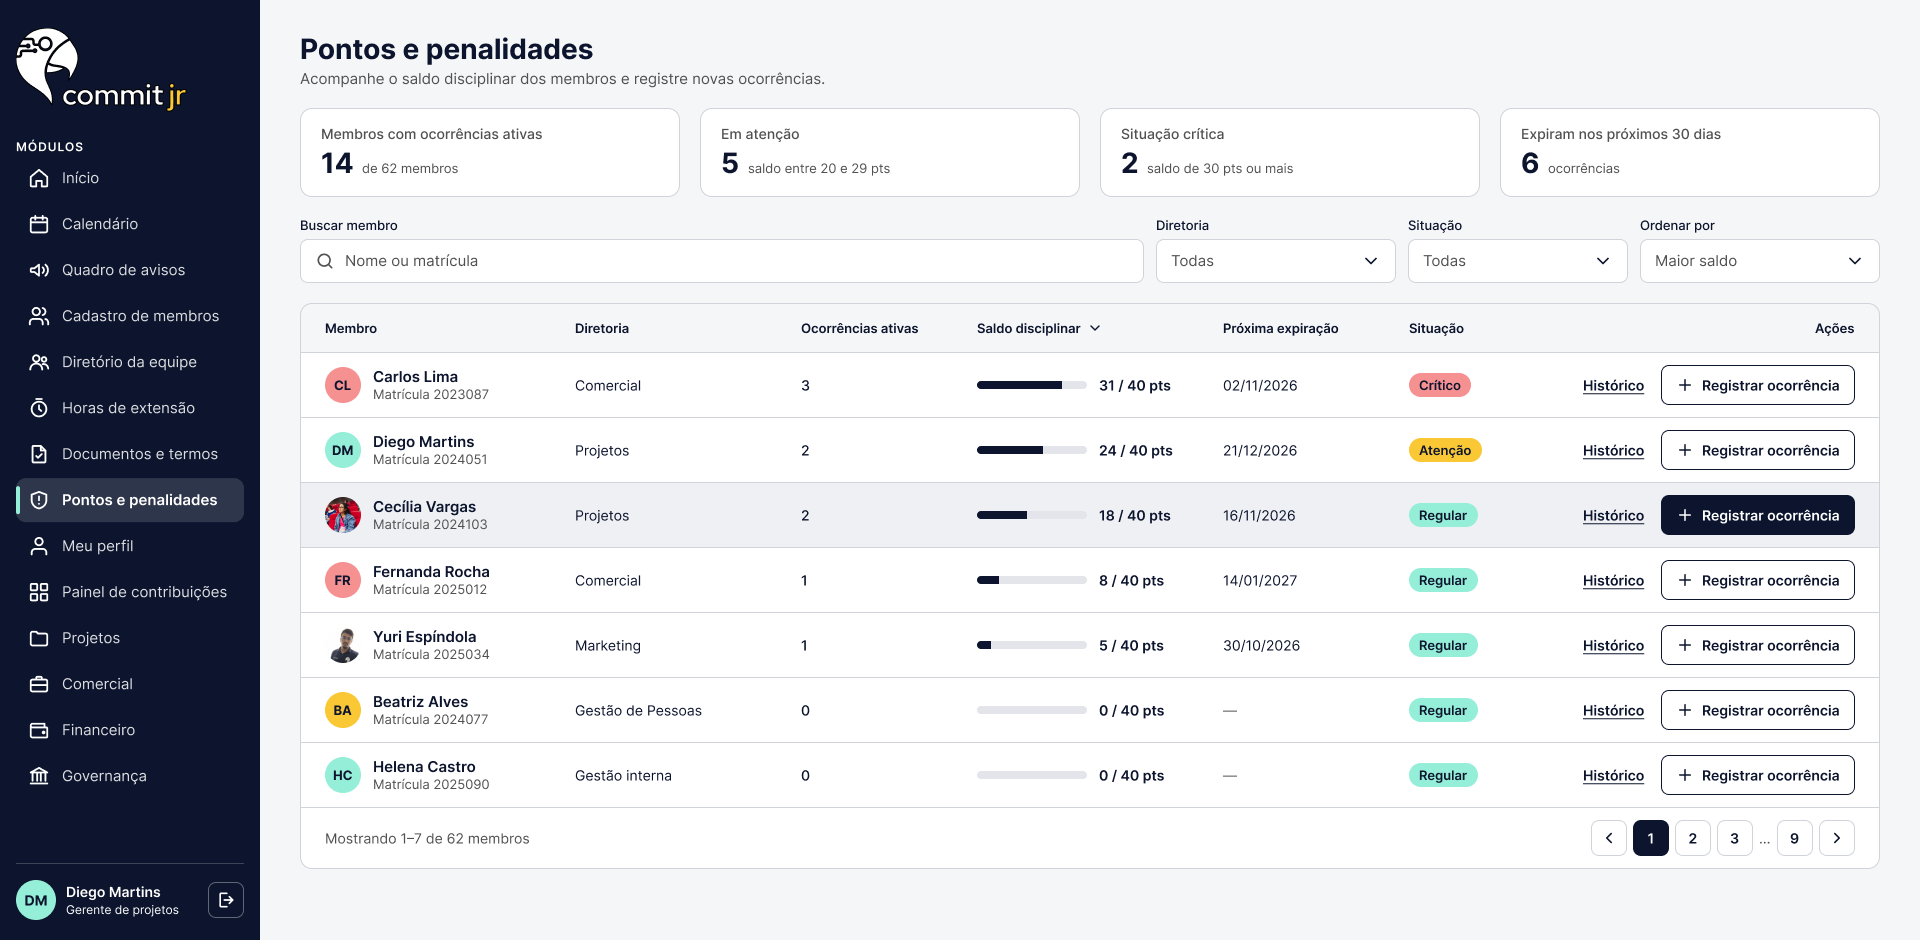
\includegraphics[width=0.88\textwidth]{Telas/pontos-lista-membros}} \\
\hline
\end{tabular}
\end{center}

\begin{center}
\begin{tabular}{|p{2.0cm}|p{11.5cm}|}
\hline
\textbf{PT-013} & \textbf{Pontos e Penalidades - Registro de Ocorrência (UC-07)} \\
\hline
\multicolumn{2}{|c|}{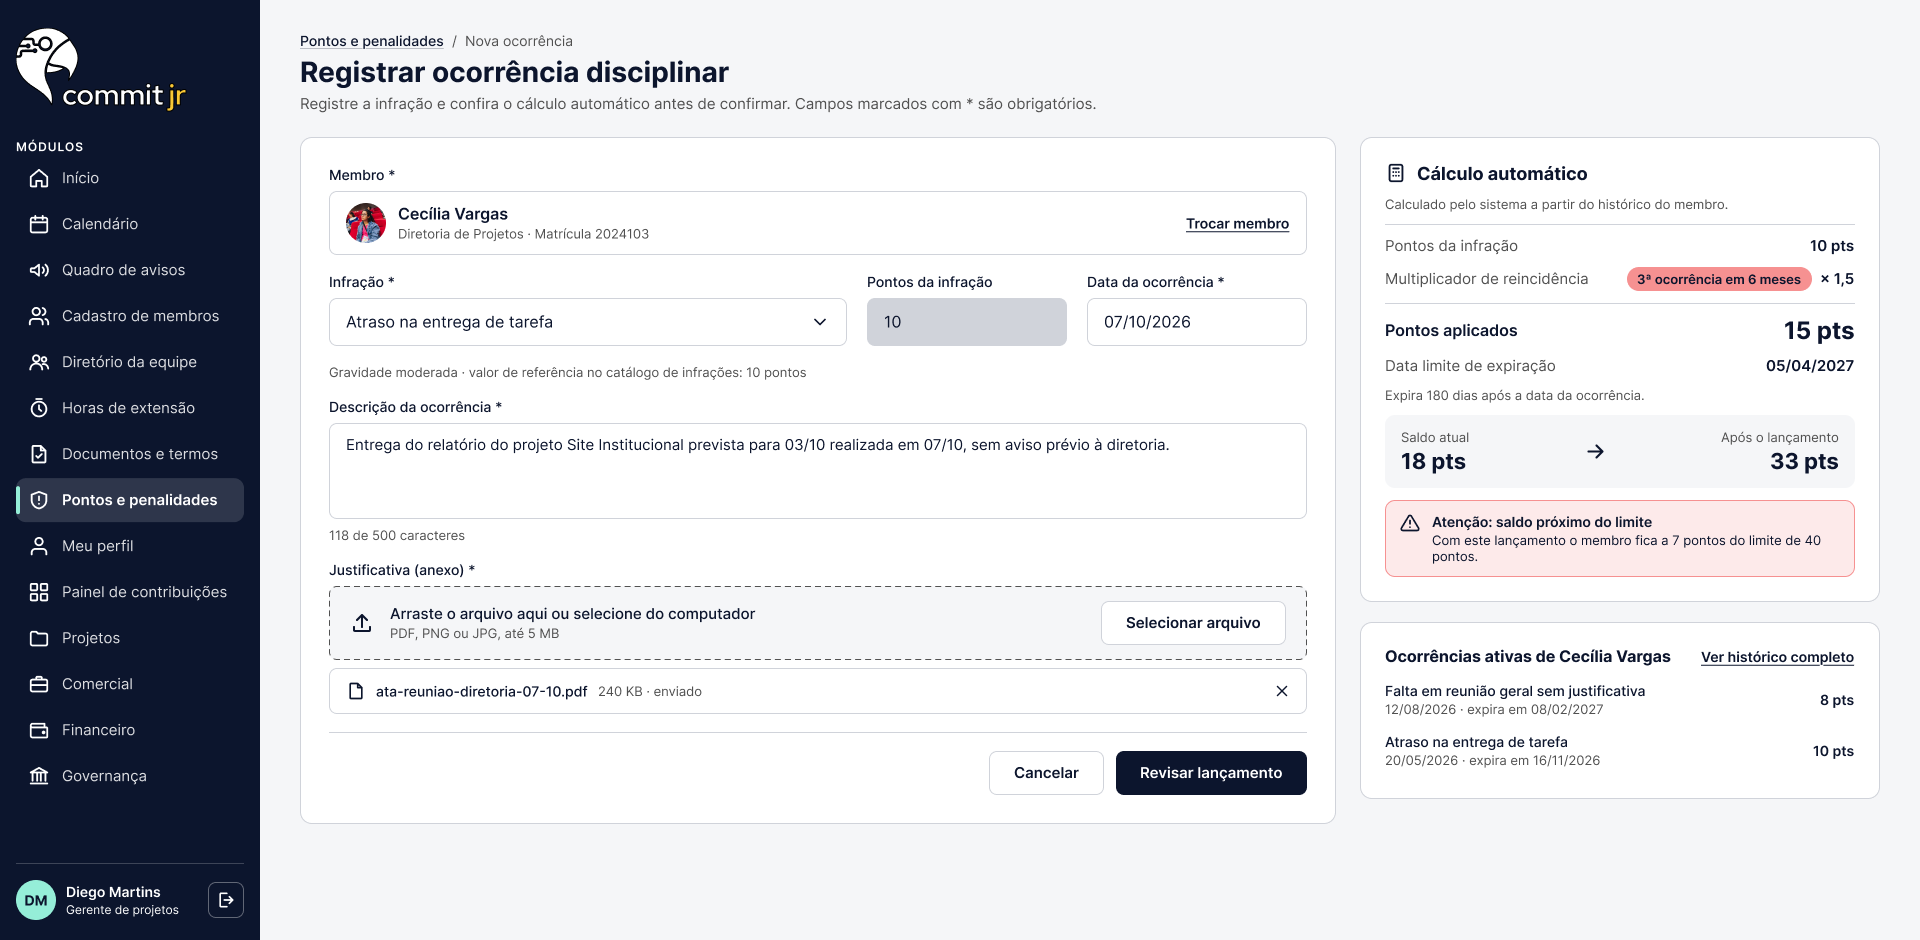
\includegraphics[width=0.88\textwidth]{Telas/pontos-registrar-ocorrencia}} \\
\hline
\end{tabular}
\end{center}

\begin{center}
\begin{tabular}{|p{2.0cm}|p{11.5cm}|}
\hline
\textbf{PT-014} & \textbf{Pontos e Penalidades - Confirmação de Lançamento (UC-07)} \\
\hline
\multicolumn{2}{|c|}{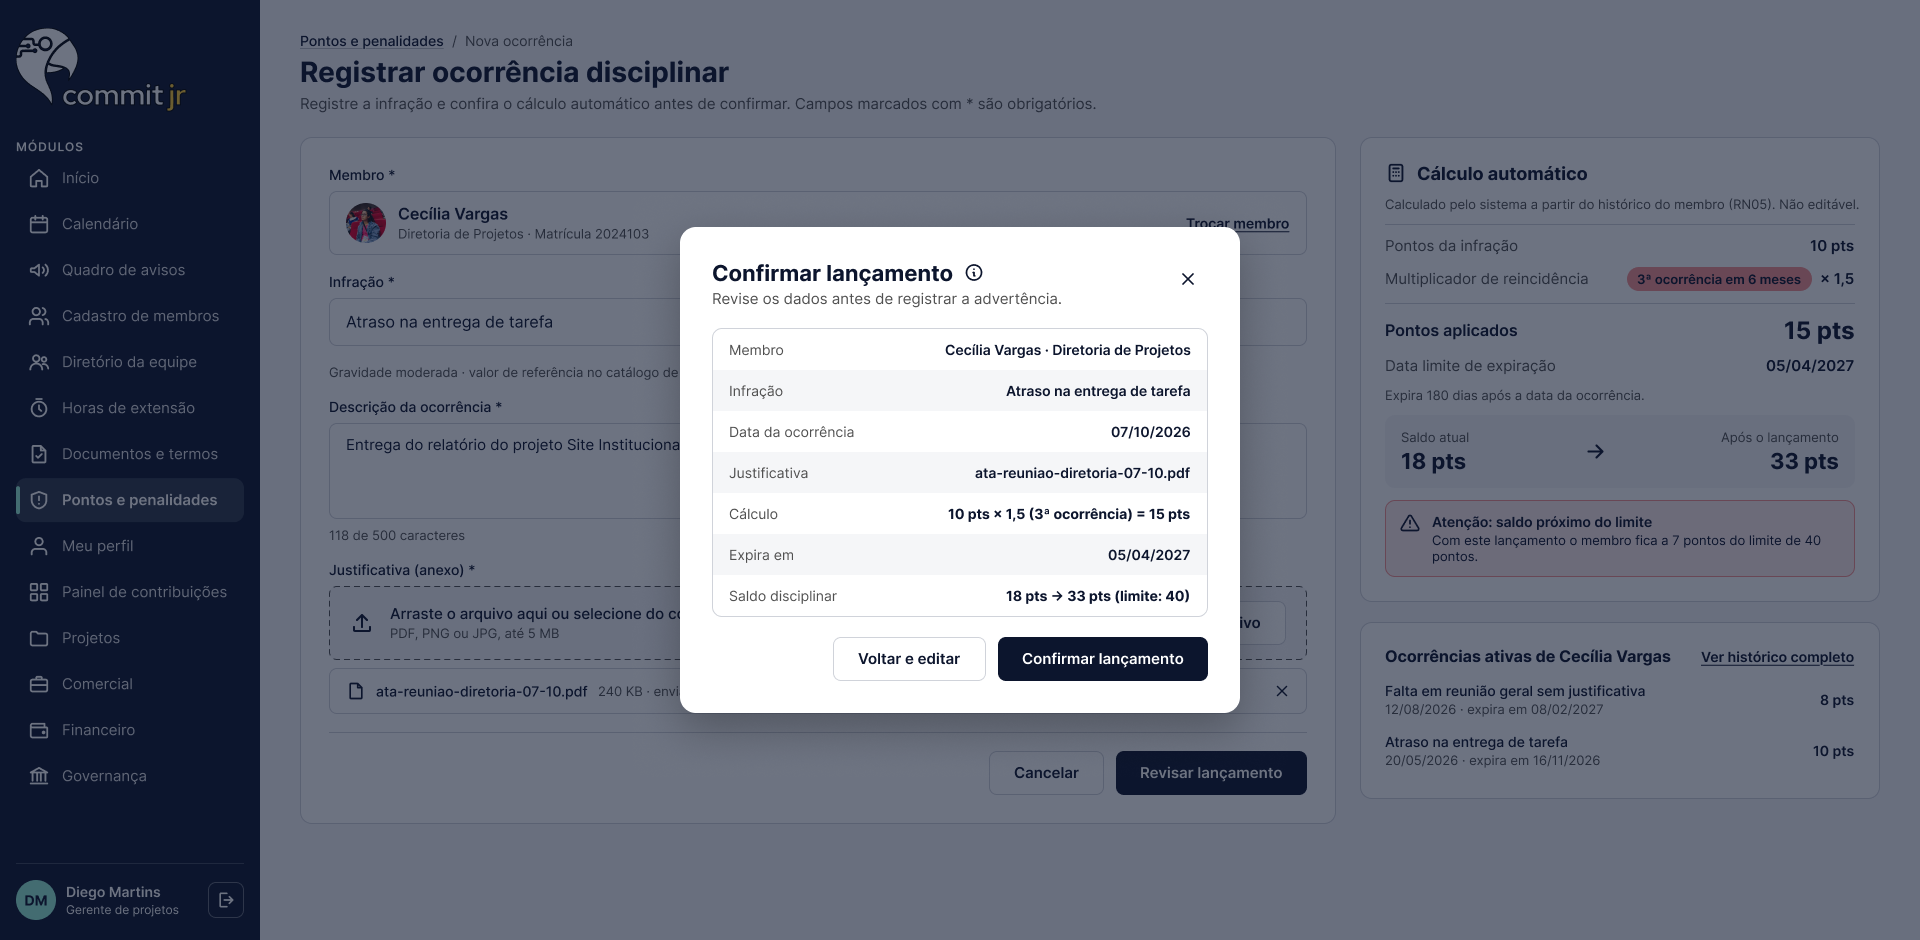
\includegraphics[width=0.88\textwidth]{Telas/pontos-confirmar-lancamento}} \\
\hline
\end{tabular}
\end{center}

\begin{center}
\begin{tabular}{|p{2.0cm}|p{11.5cm}|}
\hline
\textbf{PT-015} & \textbf{Pontos e Penalidades - Julgar Contestações (UC-08)} \\
\hline
\multicolumn{2}{|c|}{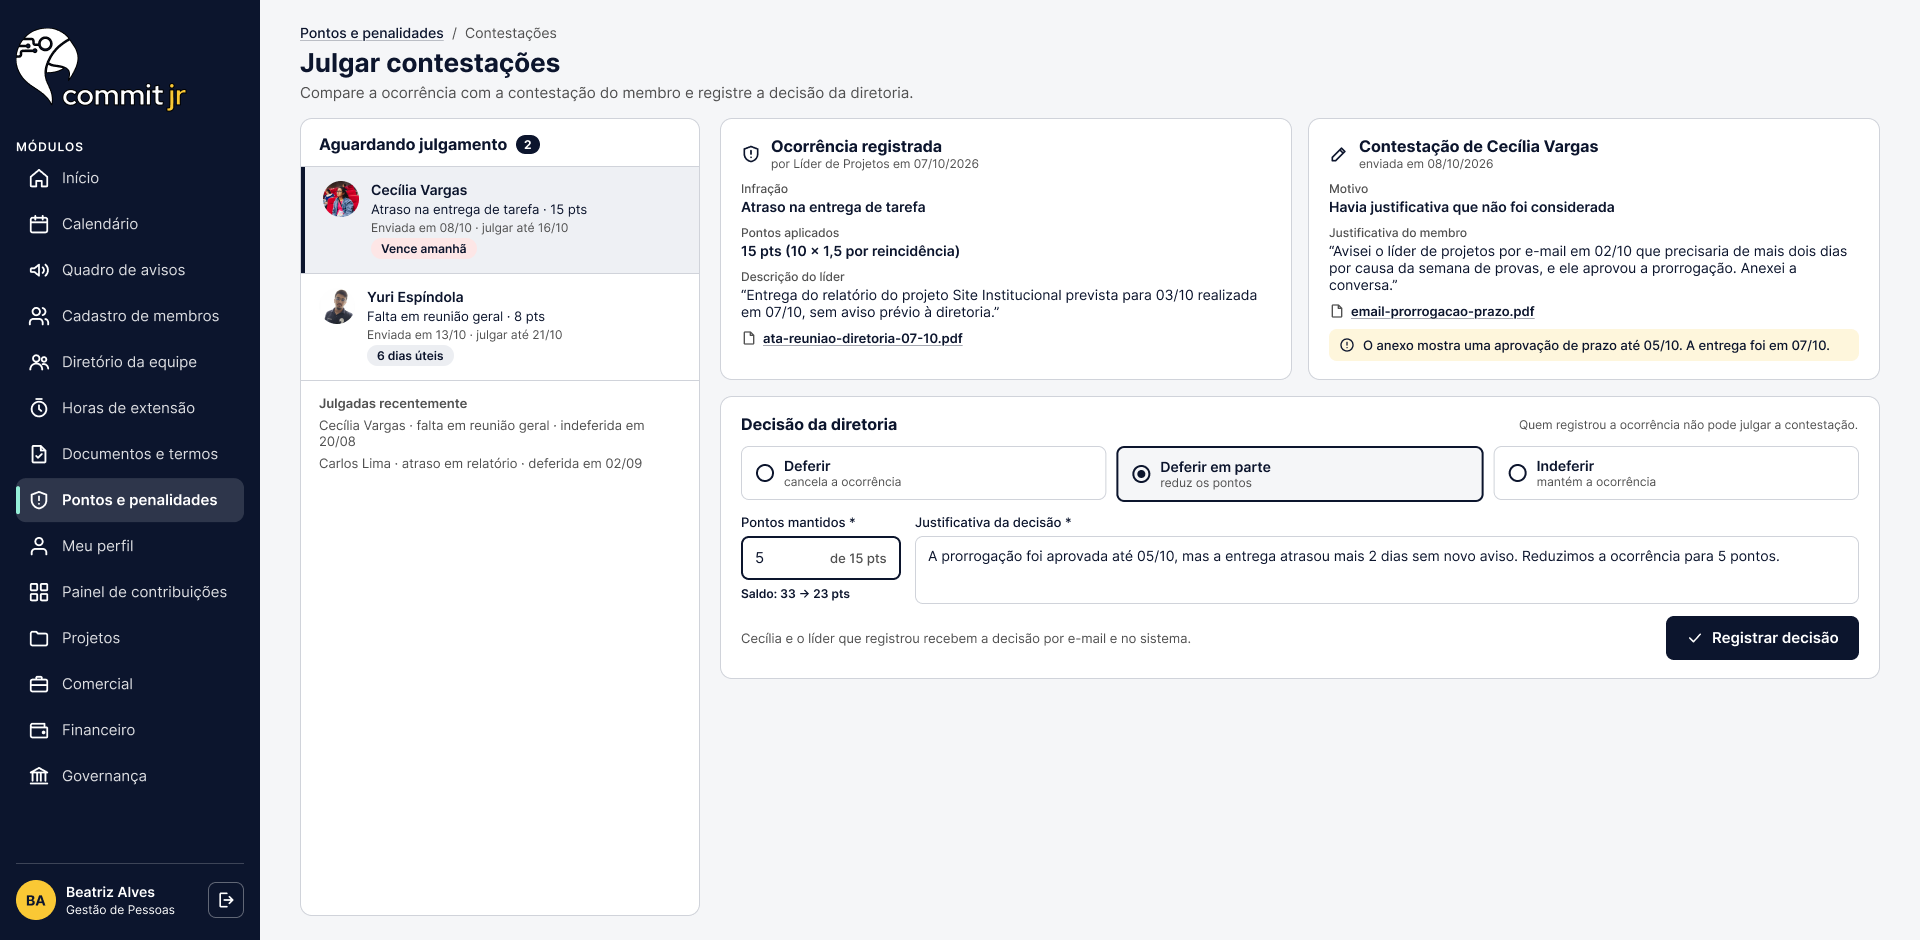
\includegraphics[width=0.88\textwidth]{Telas/pontos-julgar-contestacoes}} \\
\hline
\end{tabular}
\end{center}

\begin{center}
\begin{tabular}{|p{2.0cm}|p{11.5cm}|}
\hline
\textbf{PT-016} & \textbf{Painel do Membro - Minhas Penalidades (UC-07)} \\
\hline
\multicolumn{2}{|c|}{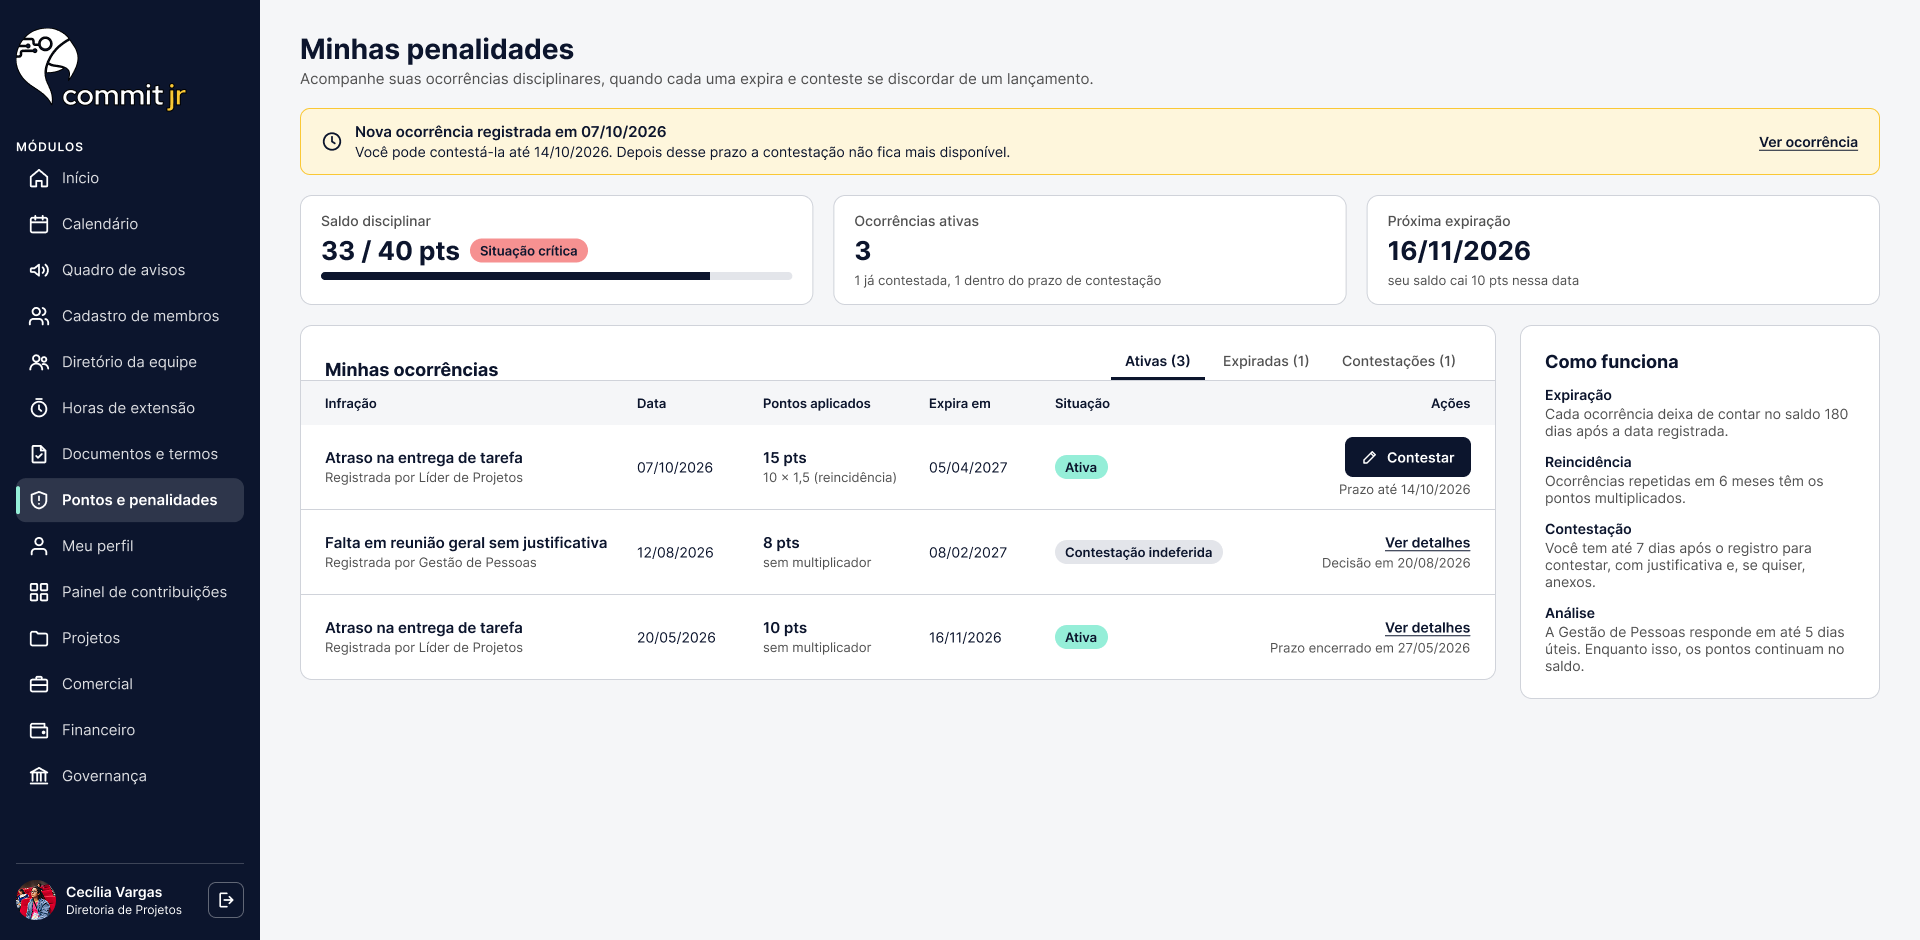
\includegraphics[width=0.88\textwidth]{Telas/pontos-membro-minhas-penalidades}} \\
\hline
\end{tabular}
\end{center}

\begin{center}
\begin{tabular}{|p{2.0cm}|p{11.5cm}|}
\hline
\textbf{PT-017} & \textbf{Painel do Membro - Contestar Ocorrência (UC-08)} \\
\hline
\multicolumn{2}{|c|}{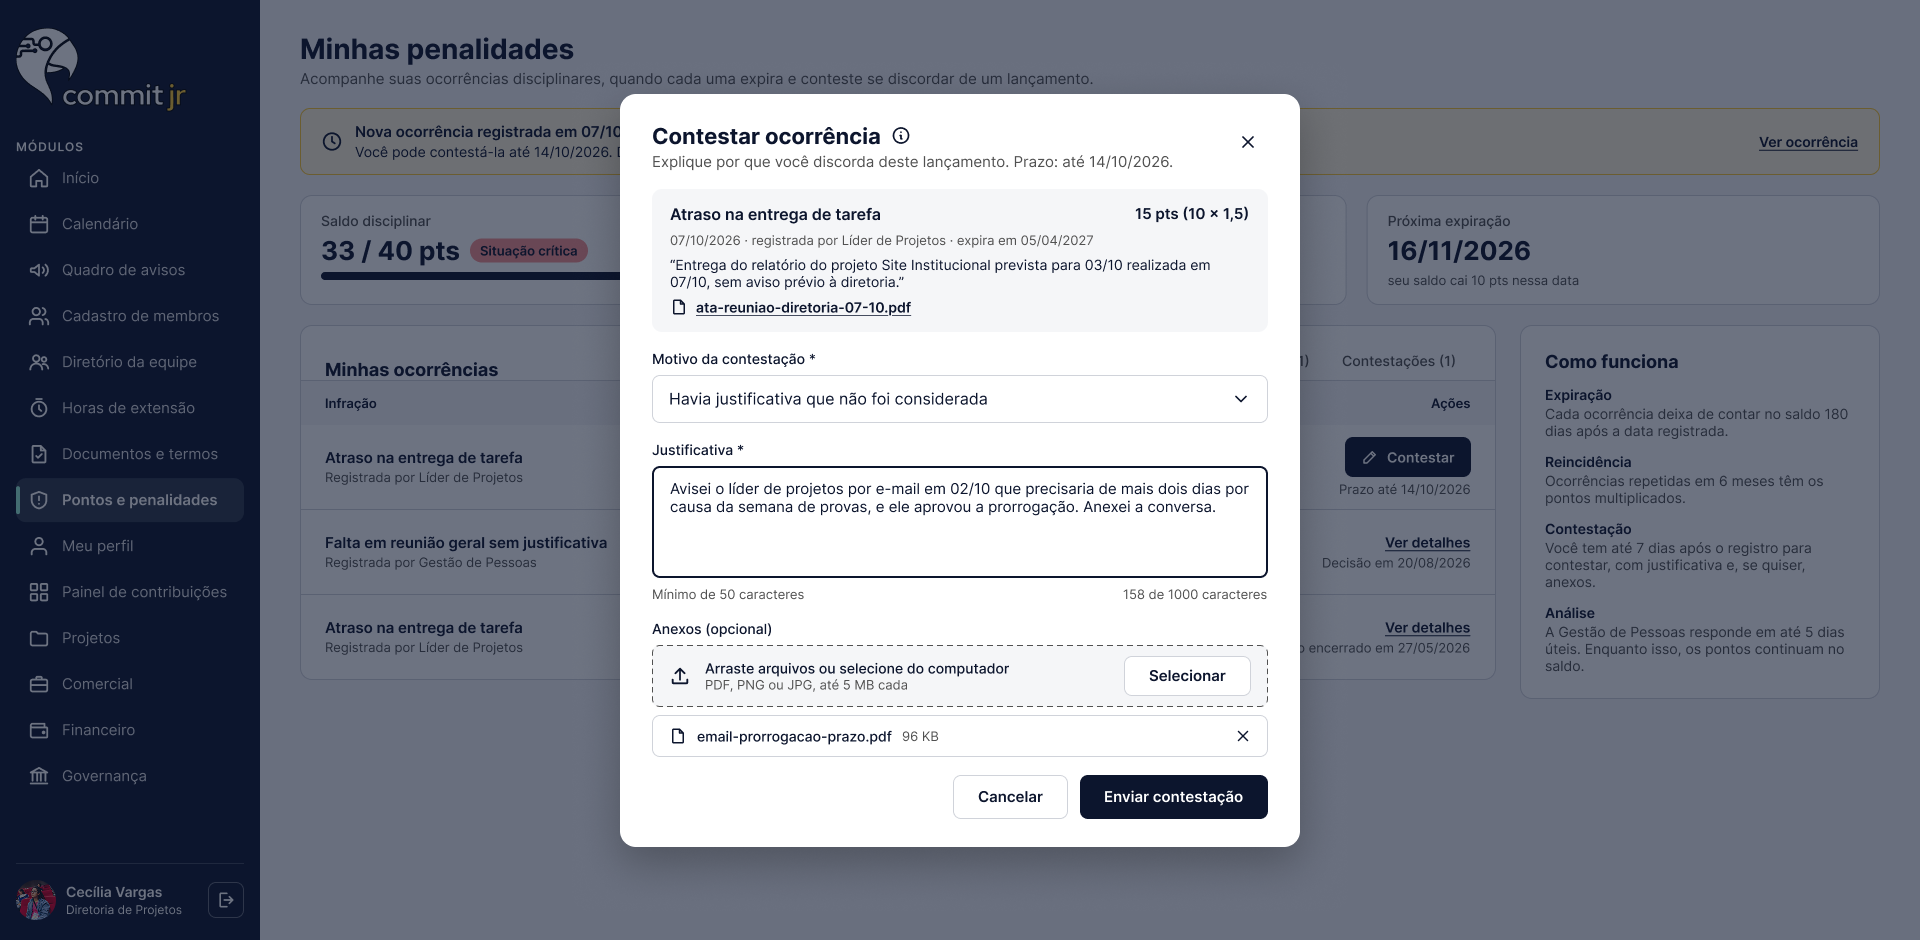
\includegraphics[width=0.88\textwidth]{Telas/pontos-membro-contestar-ocorrencia}} \\
\hline
\end{tabular}
\end{center}

\begin{center}
\begin{tabular}{|p{2.0cm}|p{11.5cm}|}
\hline
\textbf{PT-018} & \textbf{Painel do Membro - Contestação Enviada (UC-08)} \\
\hline
\multicolumn{2}{|c|}{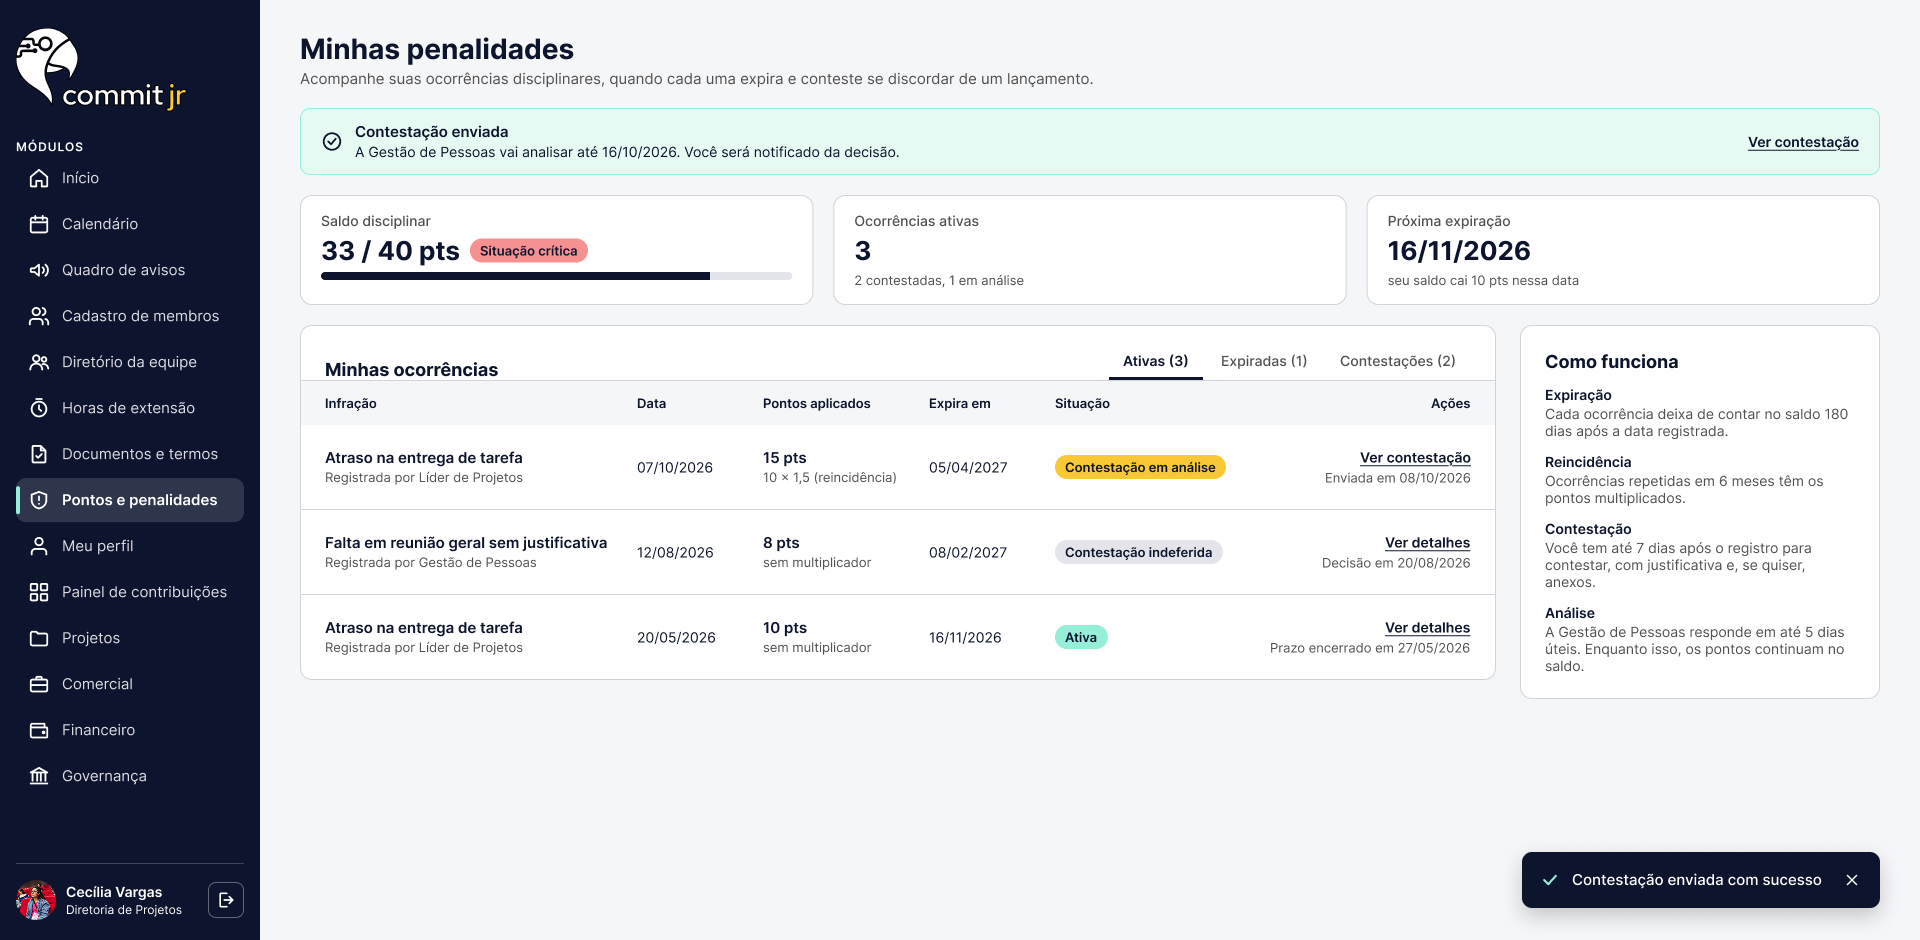
\includegraphics[width=0.88\textwidth]{Telas/pontos-membro-contestacao-enviada}} \\
\hline
\end{tabular}
\end{center}

\begin{center}
\begin{tabular}{|p{2.0cm}|p{11.5cm}|}
\hline
\textbf{PT-019} & \textbf{Quadro de Avisos - Publicar Aviso (UC-10)} \\
\hline
\multicolumn{2}{|c|}{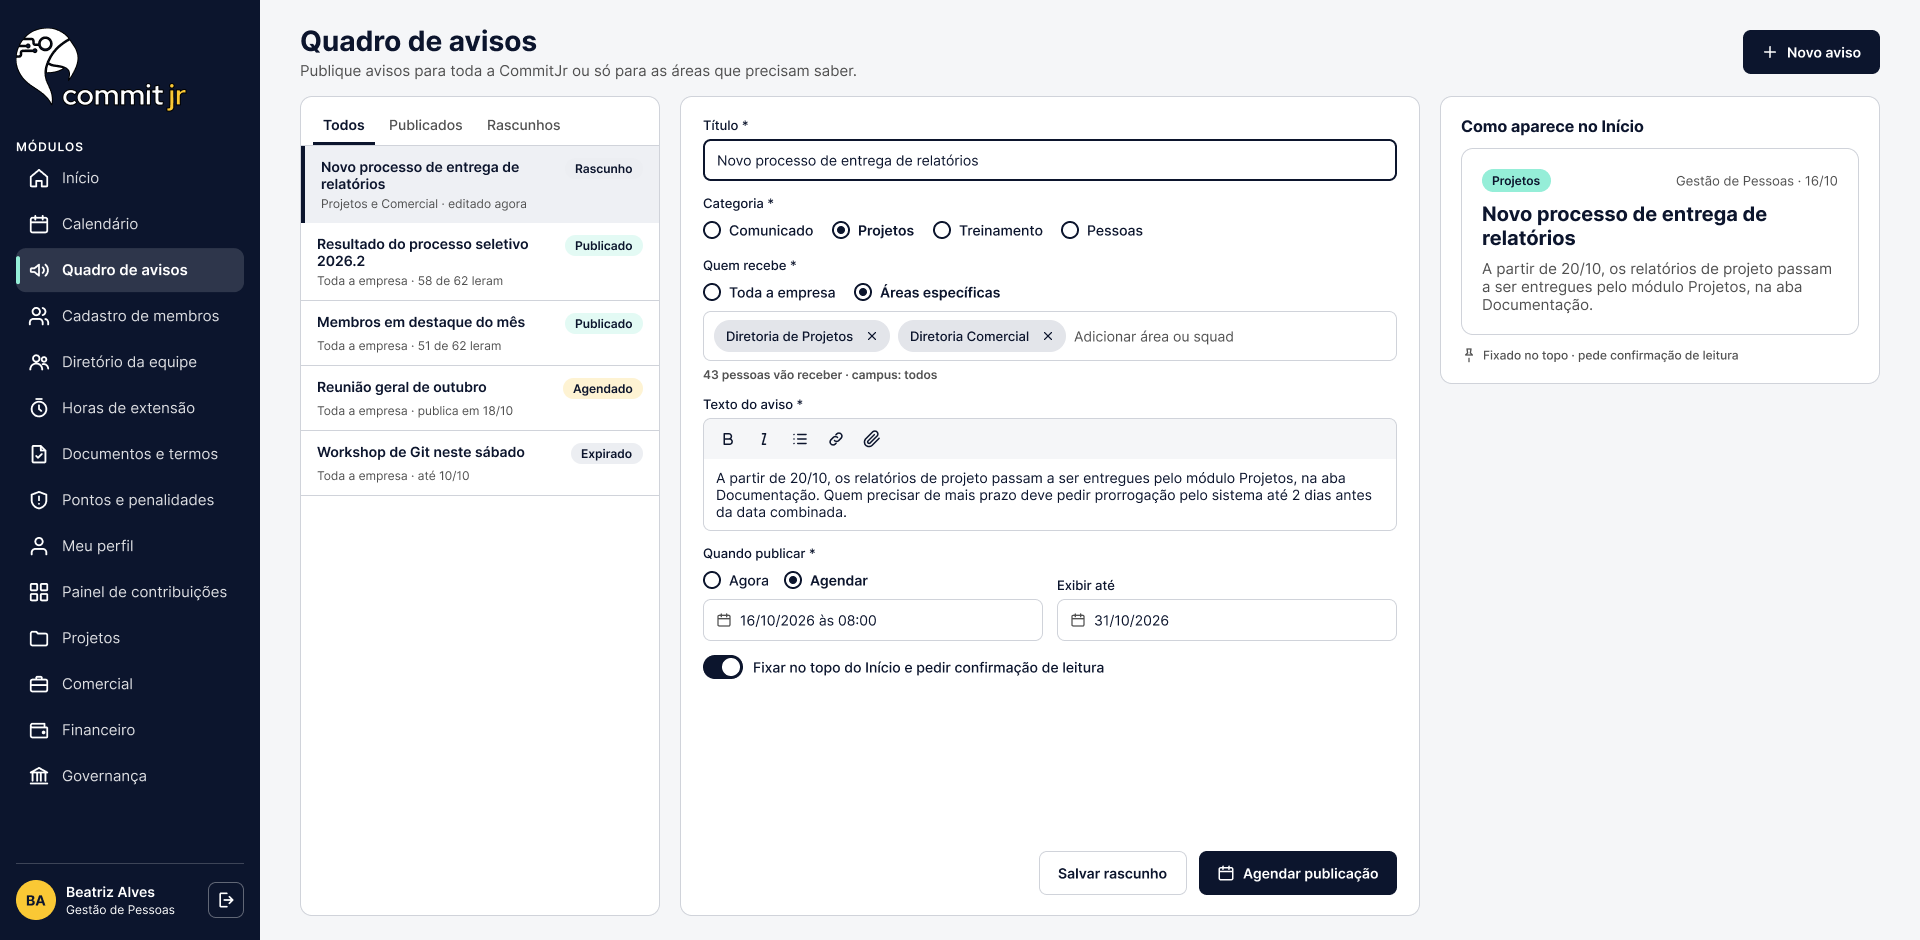
\includegraphics[width=0.88\textwidth]{Telas/quadro-avisos-publicar}} \\
\hline
\end{tabular}
\end{center}

\begin{center}
\begin{tabular}{|p{2.0cm}|p{11.5cm}|}
\hline
\textbf{PT-020} & \textbf{Calendário Corporativo - Visão Mensal (UC-11)} \\
\hline
\multicolumn{2}{|c|}{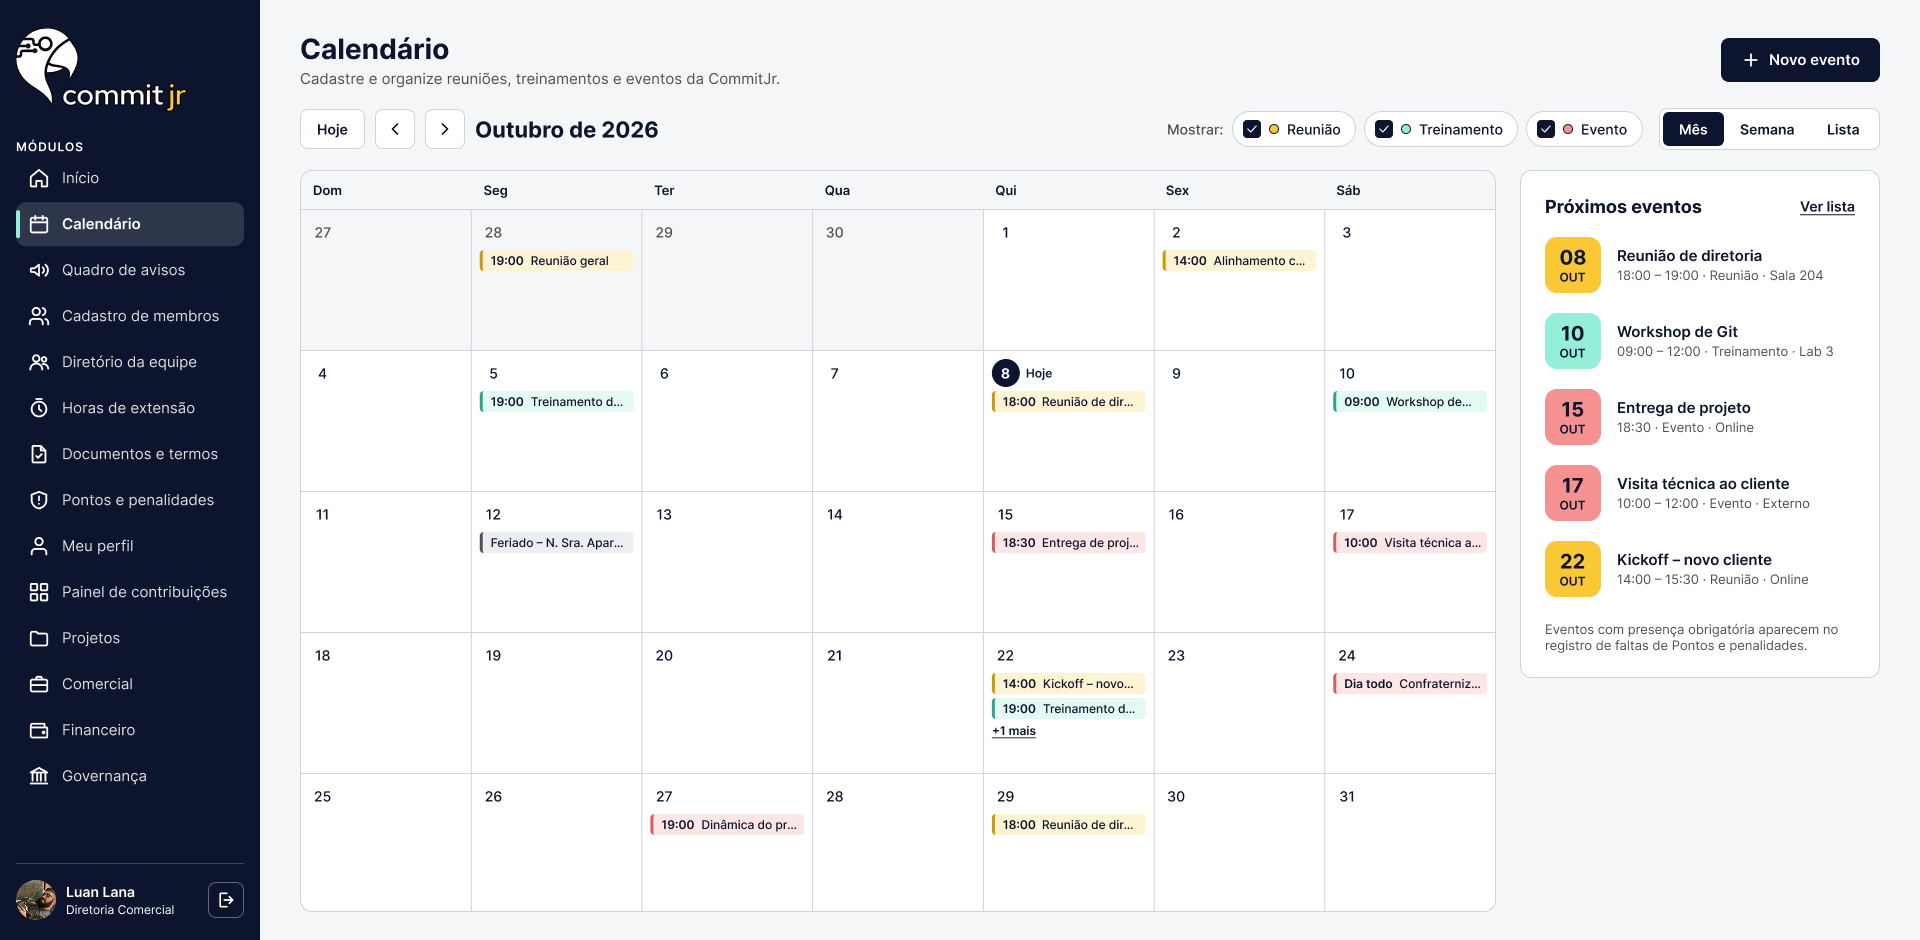
\includegraphics[width=0.88\textwidth]{Telas/calendario-visao-mensal}} \\
\hline
\end{tabular}
\end{center}

\begin{center}
\begin{tabular}{|p{2.0cm}|p{11.5cm}|}
\hline
\textbf{PT-021} & \textbf{Calendário Corporativo - Novo Evento Institucional (UC-11)} \\
\hline
\multicolumn{2}{|c|}{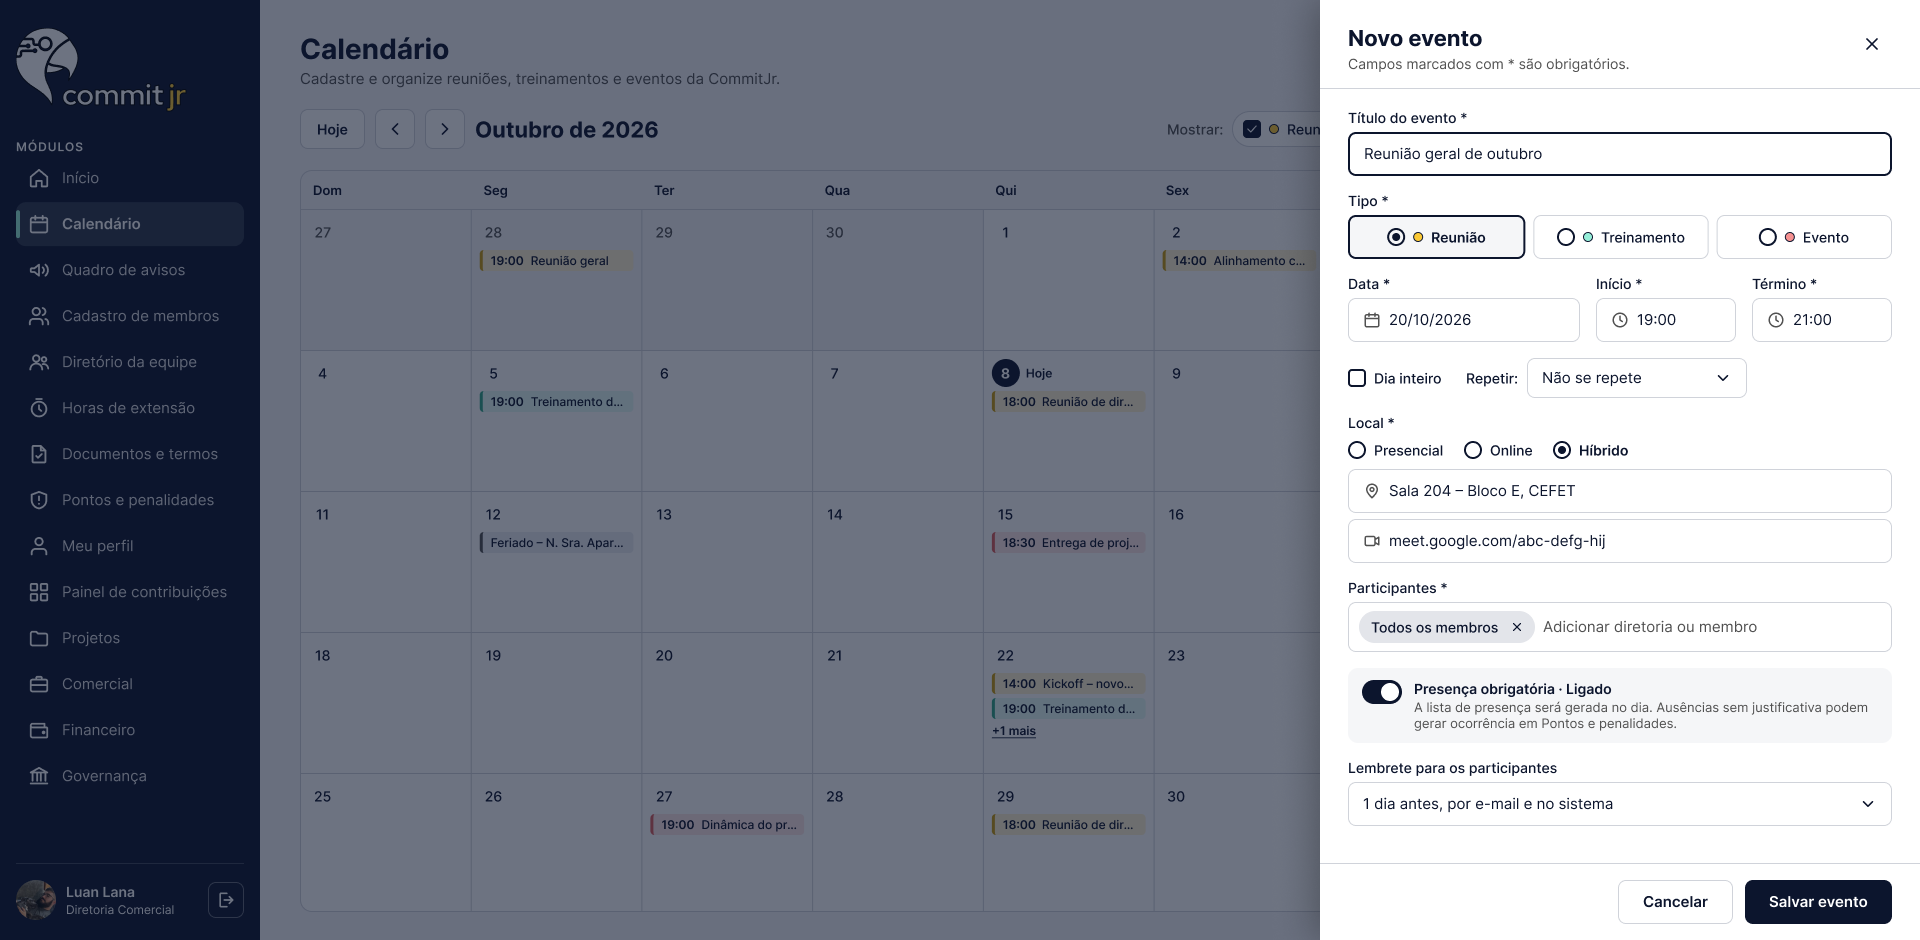
\includegraphics[width=0.88\textwidth]{Telas/calendario-novo-evento}} \\
\hline
\end{tabular}
\end{center}

\begin{center}
\begin{tabular}{|p{2.0cm}|p{11.5cm}|}
\hline
\textbf{PT-022} & \textbf{Calendário Corporativo - Agendar Reunião 1-on-1 (UC-11)} \\
\hline
\multicolumn{2}{|c|}{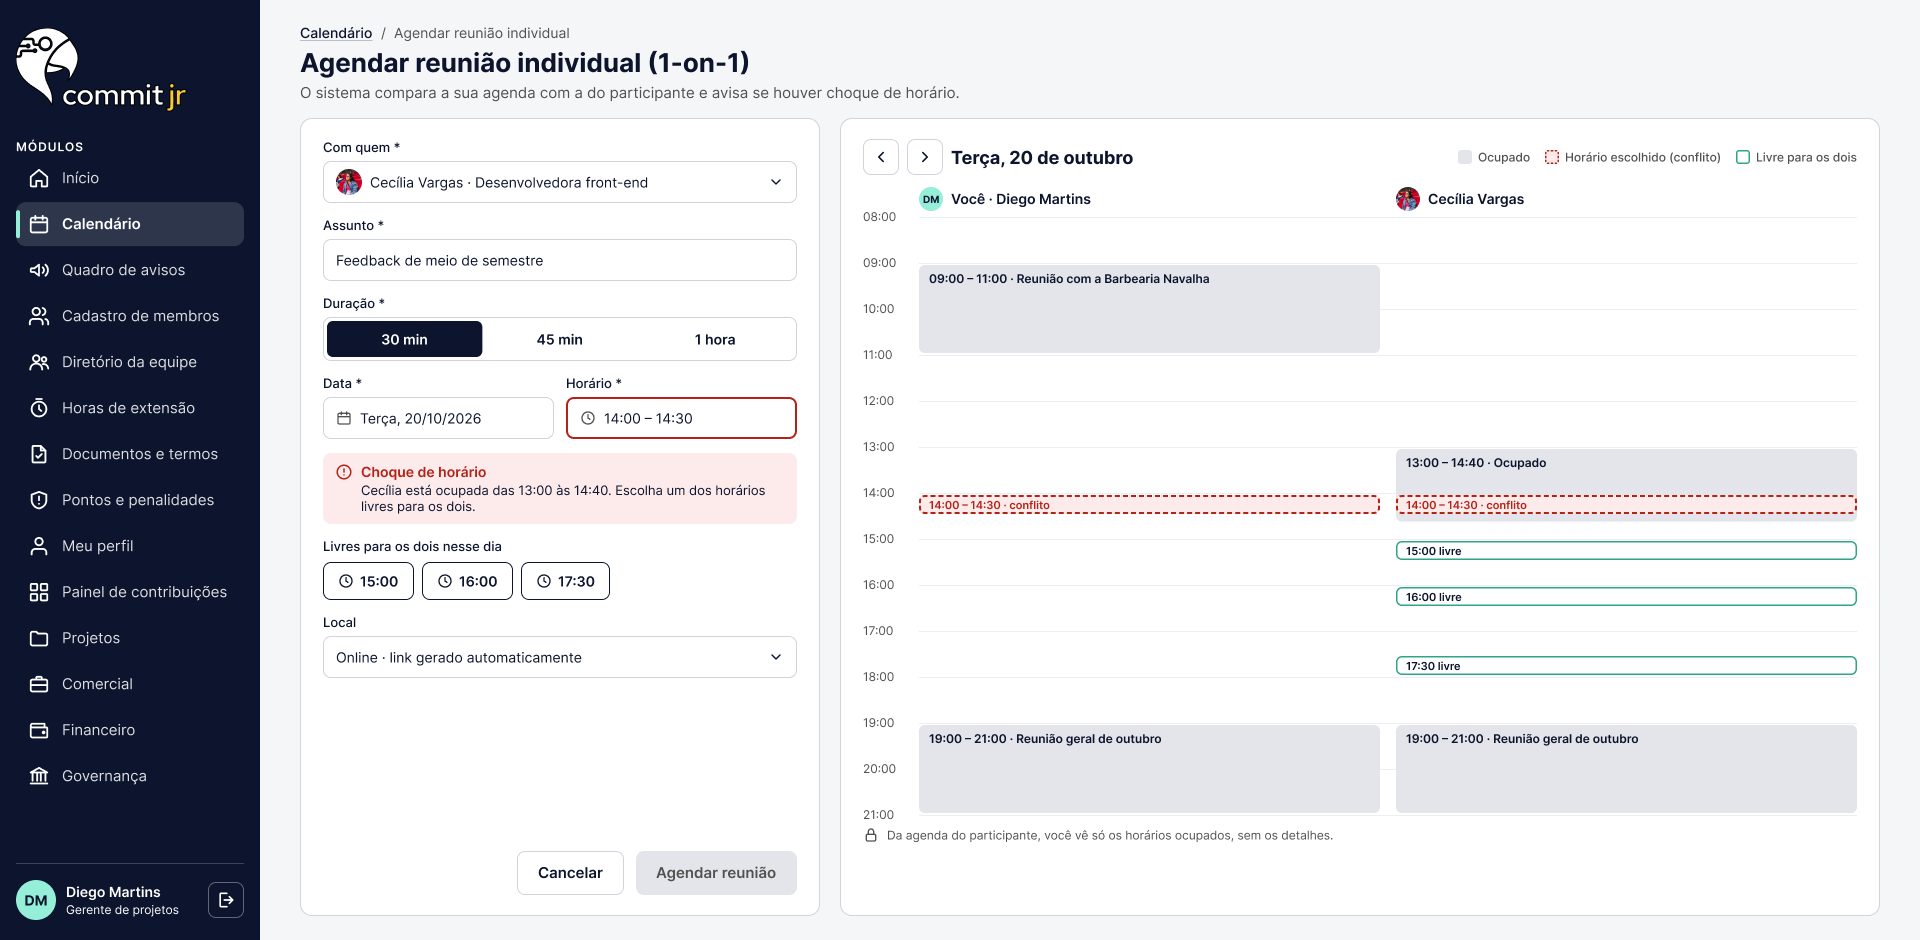
\includegraphics[width=0.88\textwidth]{Telas/calendario-agendar-1on1}} \\
\hline
\end{tabular}
\end{center}

\begin{center}
\begin{tabular}{|p{2.0cm}|p{11.5cm}|}
\hline
\textbf{PT-023} & \textbf{Calendário Corporativo - Confirmação de Evento Salvo (UC-11)} \\
\hline
\multicolumn{2}{|c|}{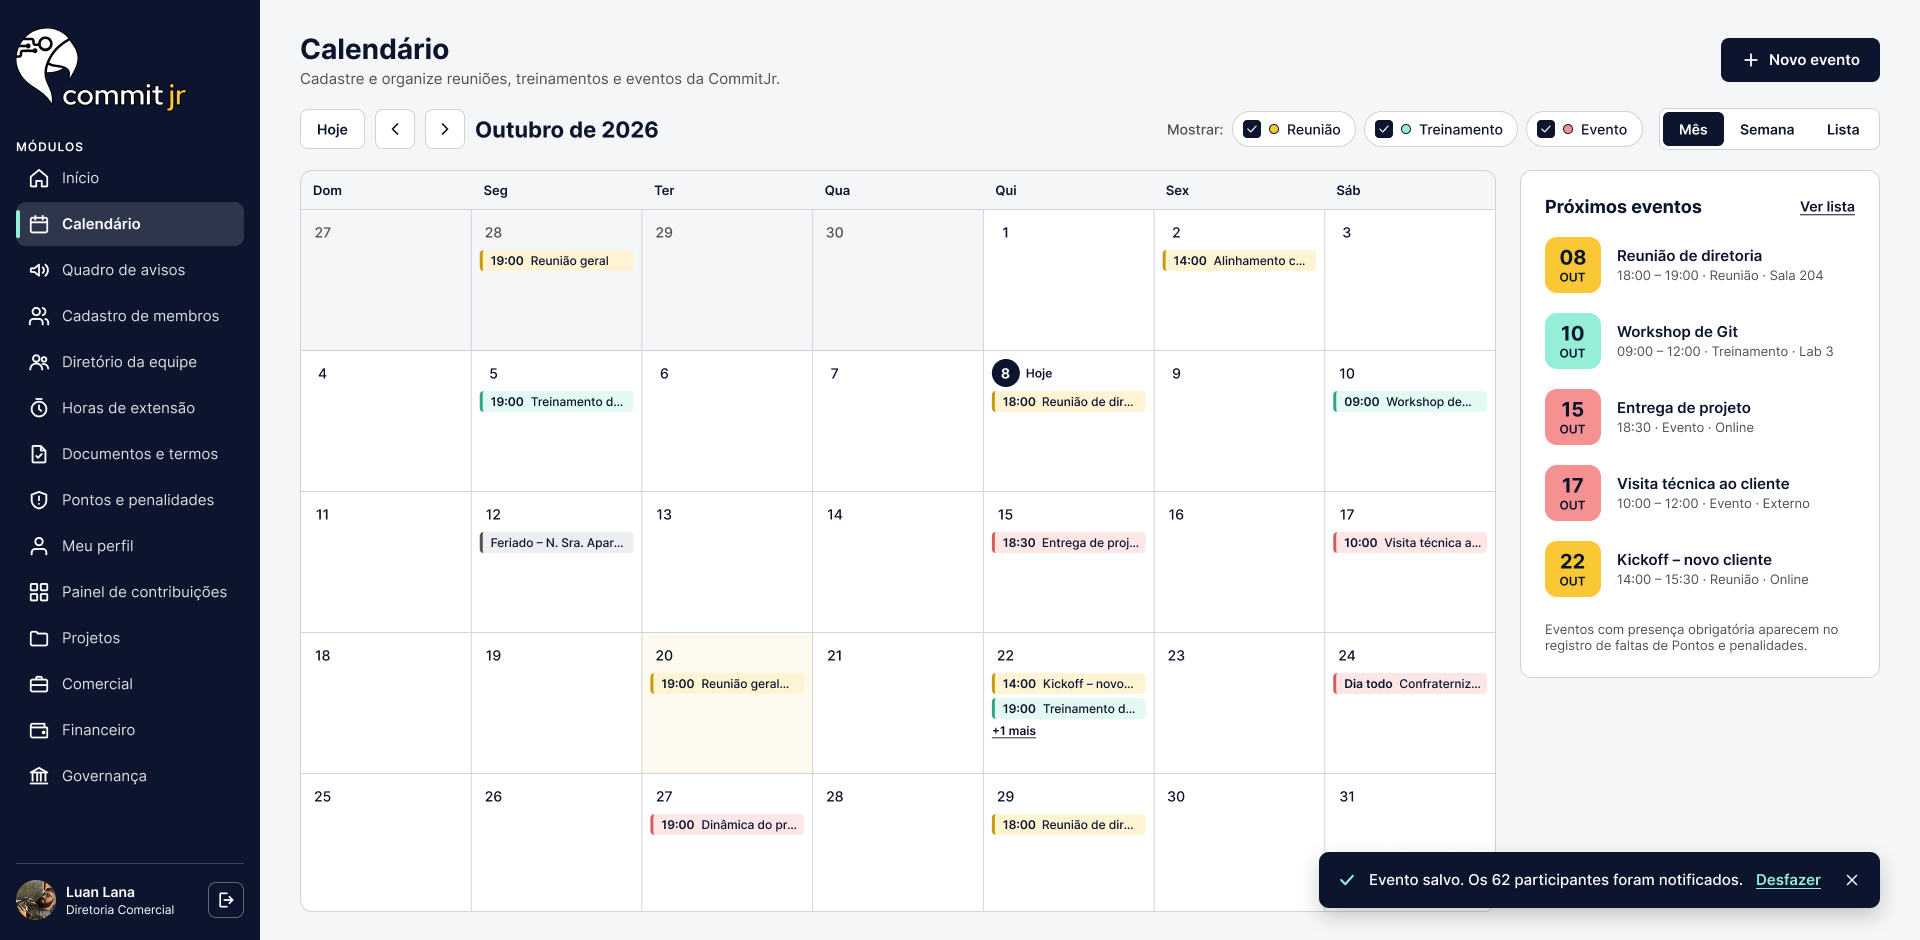
\includegraphics[width=0.88\textwidth]{Telas/calendario-evento-salvo}} \\
\hline
\end{tabular}
\end{center}

\begin{center}
\begin{tabular}{|p{2.0cm}|p{11.5cm}|}
\hline
\textbf{PT-024} & \textbf{Governança - Gestão de Perfis de Acesso} \\
\hline
\multicolumn{2}{|c|}{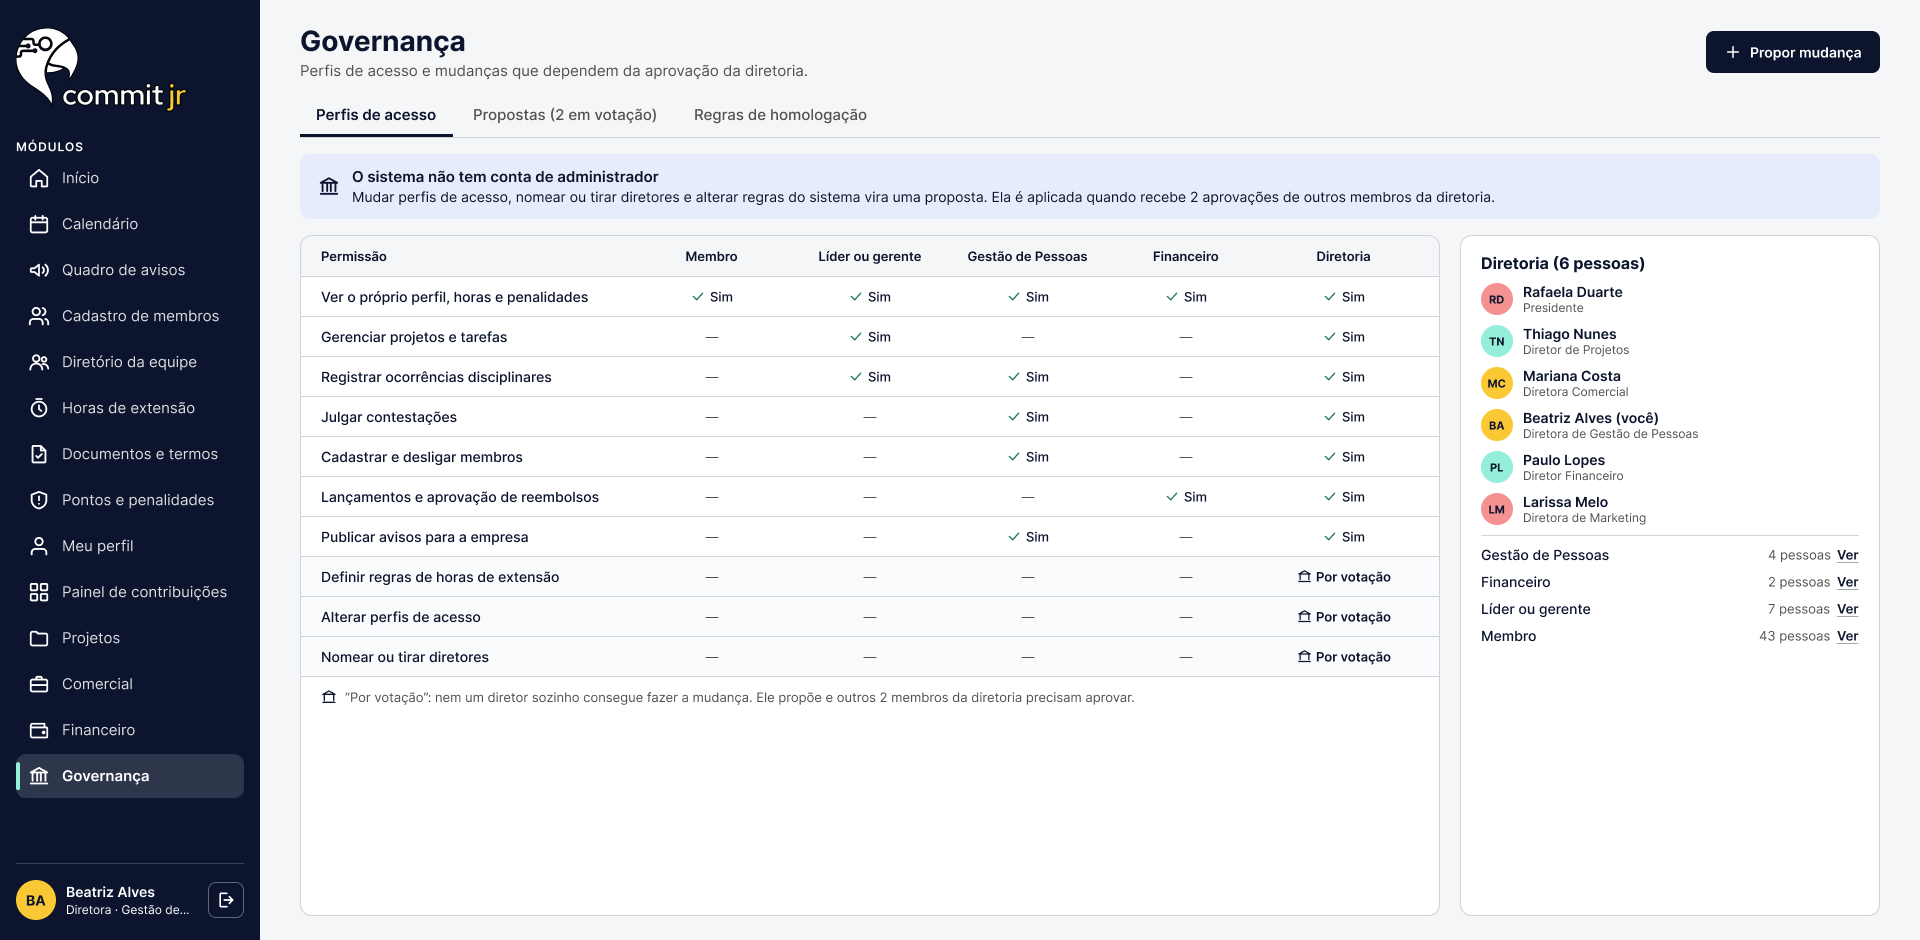
\includegraphics[width=0.88\textwidth]{Telas/governanca-perfis-acesso}} \\
\hline
\end{tabular}
\end{center}

\begin{center}
\begin{tabular}{|p{2.0cm}|p{11.5cm}|}
\hline
\textbf{PT-025} & \textbf{Governança - Homologar Proposta Institucional} \\
\hline
\multicolumn{2}{|c|}{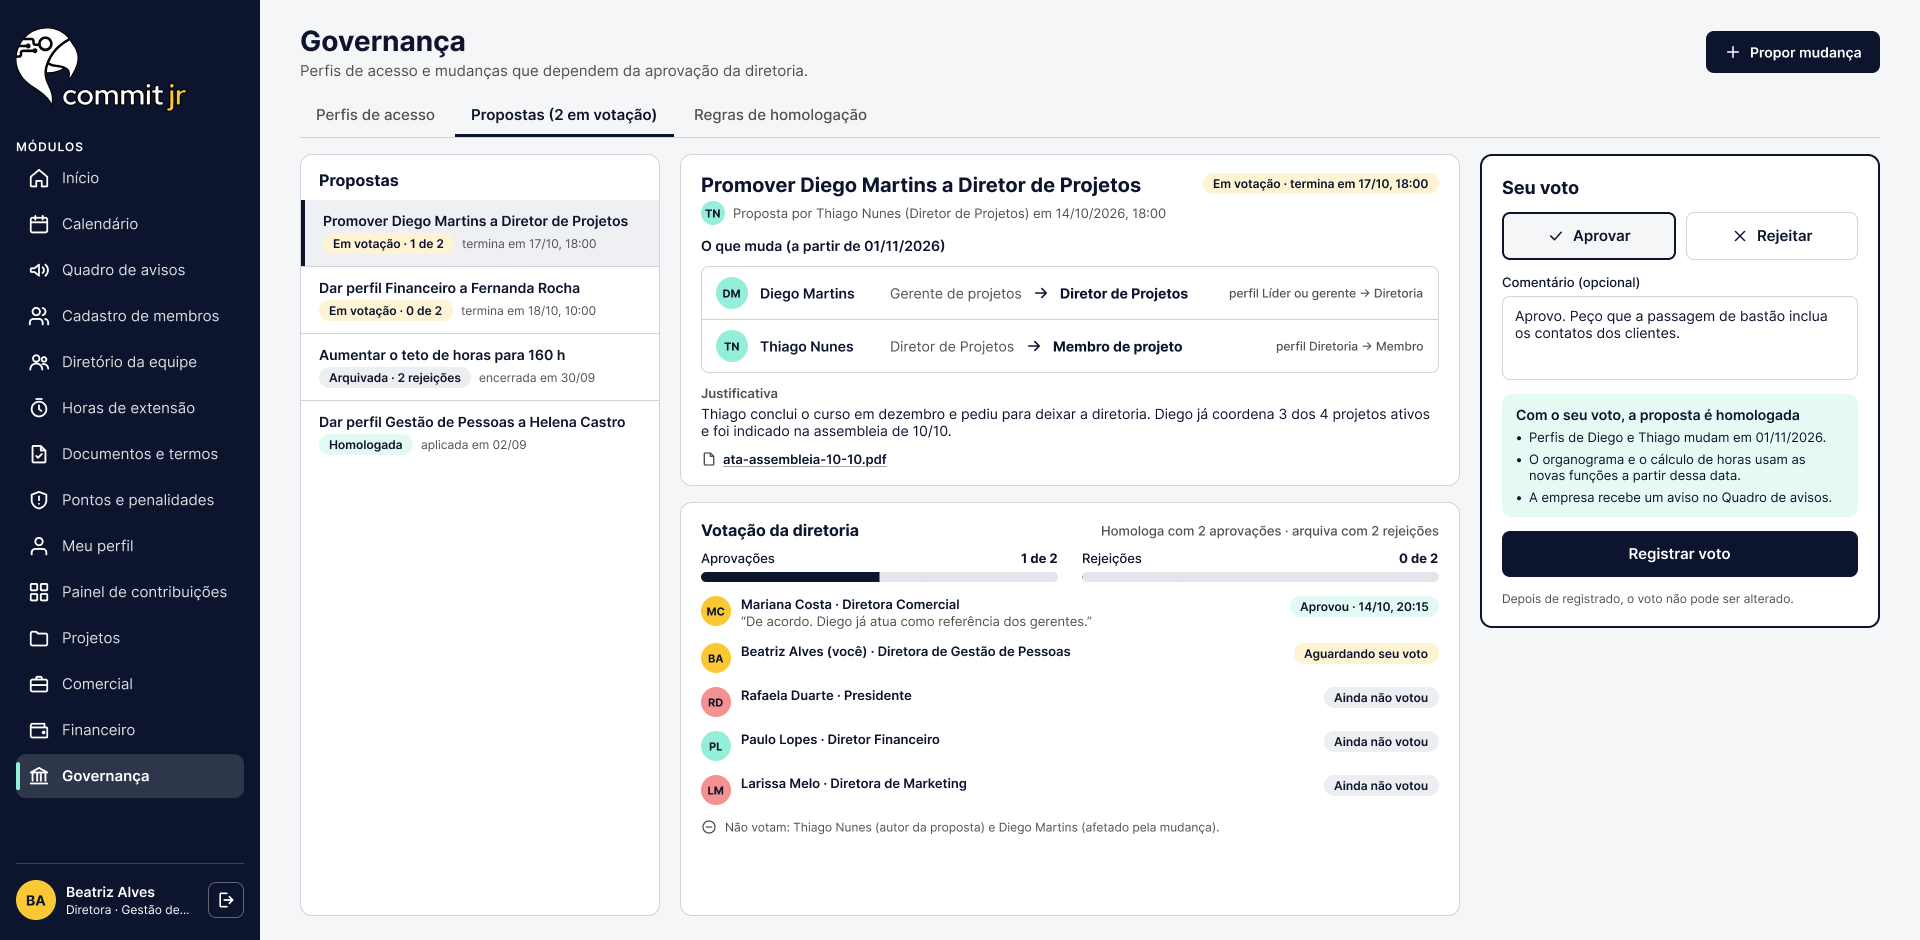
\includegraphics[width=0.88\textwidth]{Telas/governanca-homologar-proposta}} \\
\hline
\end{tabular}
\end{center}

\begin{center}
\begin{tabular}{|p{2.0cm}|p{11.5cm}|}
\hline
\textbf{PT-026} & \textbf{Gestão de Projetos - Visão do Gerente} \\
\hline
\multicolumn{2}{|c|}{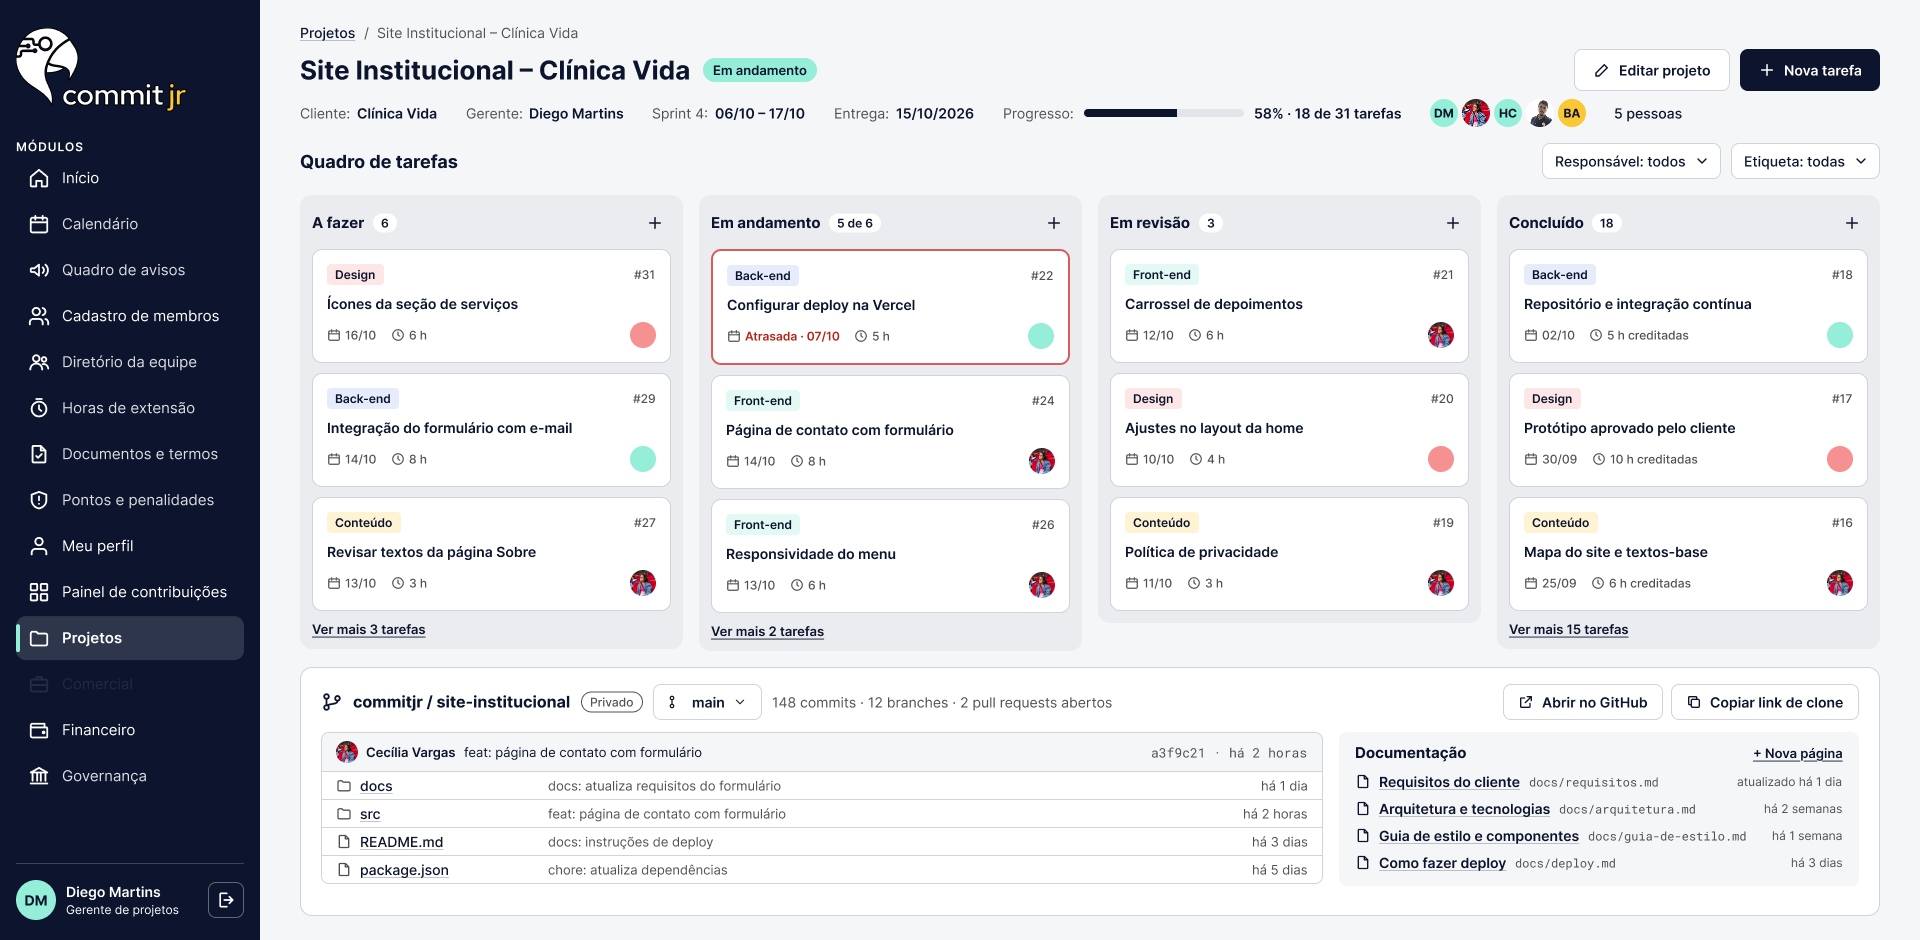
\includegraphics[width=0.88\textwidth]{Telas/projetos-visao-gerente}} \\
\hline
\end{tabular}
\end{center}

\begin{center}
\begin{tabular}{|p{2.0cm}|p{11.5cm}|}
\hline
\textbf{PT-027} & \textbf{Gestão de Projetos - Lista Geral (Gerente)} \\
\hline
\multicolumn{2}{|c|}{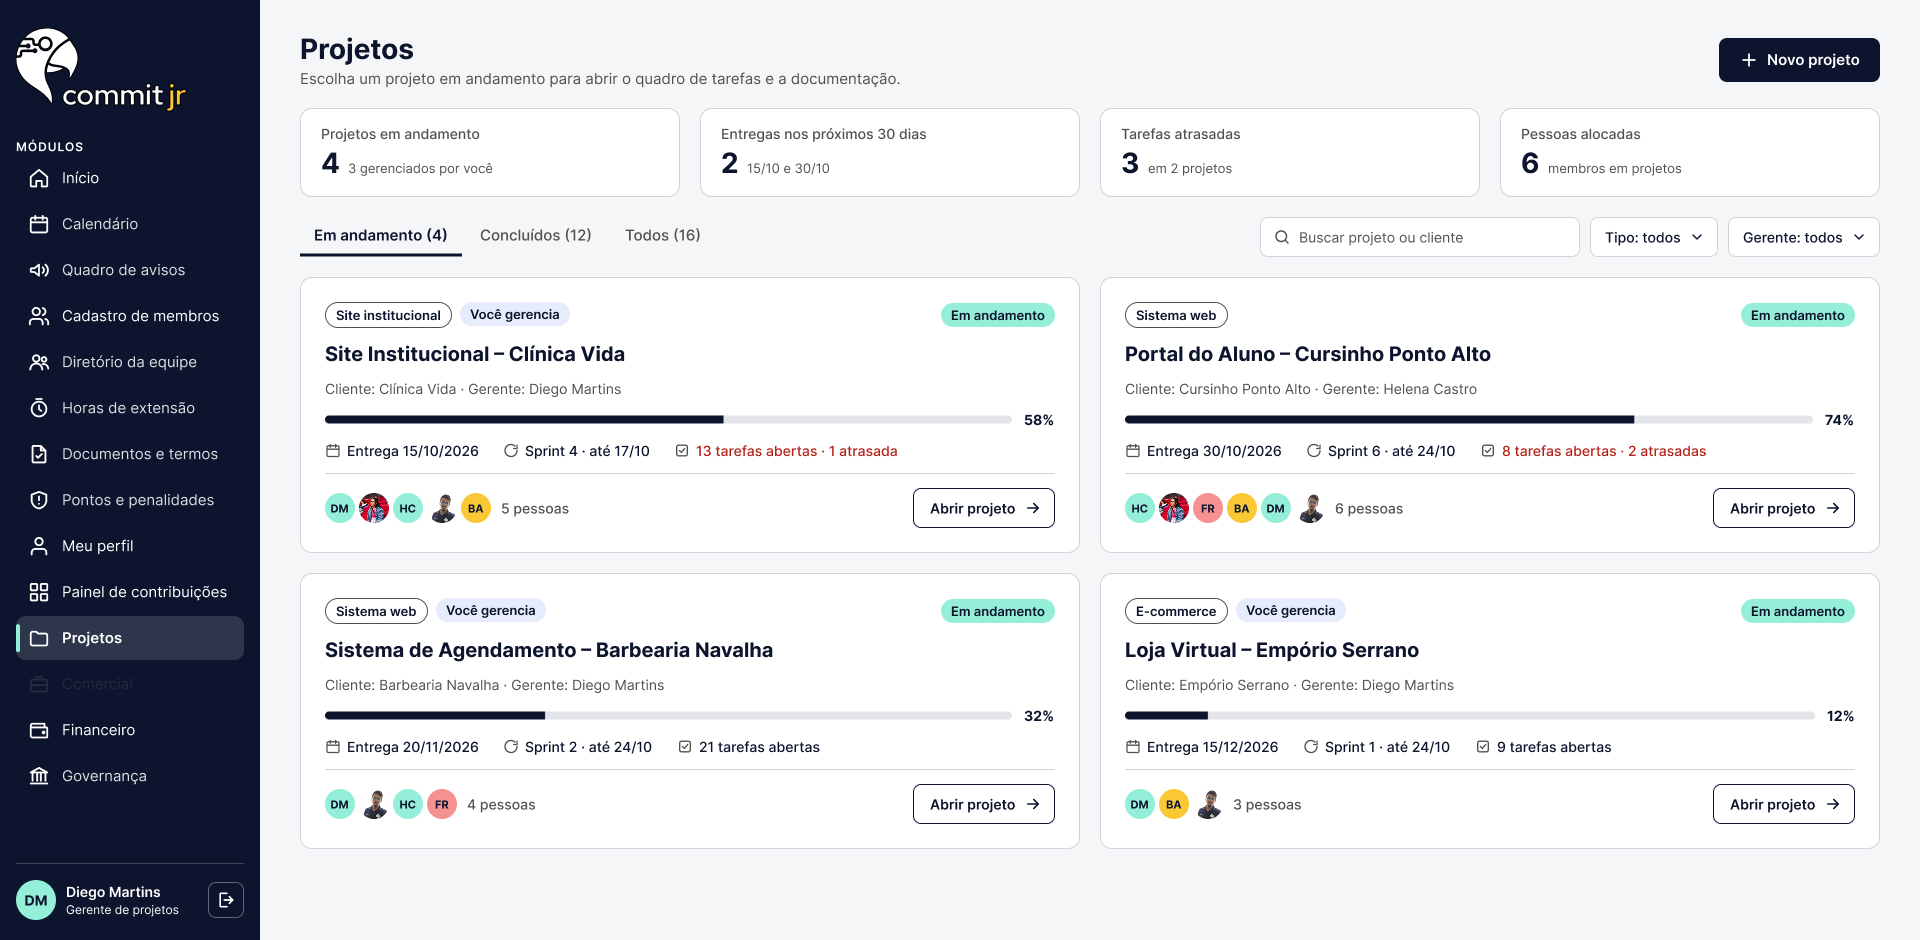
\includegraphics[width=0.88\textwidth]{Telas/projetos-lista-gerente}} \\
\hline
\end{tabular}
\end{center}

\begin{center}
\begin{tabular}{|p{2.0cm}|p{11.5cm}|}
\hline
\textbf{PT-028} & \textbf{Gestão de Projetos - Visão do Membro} \\
\hline
\multicolumn{2}{|c|}{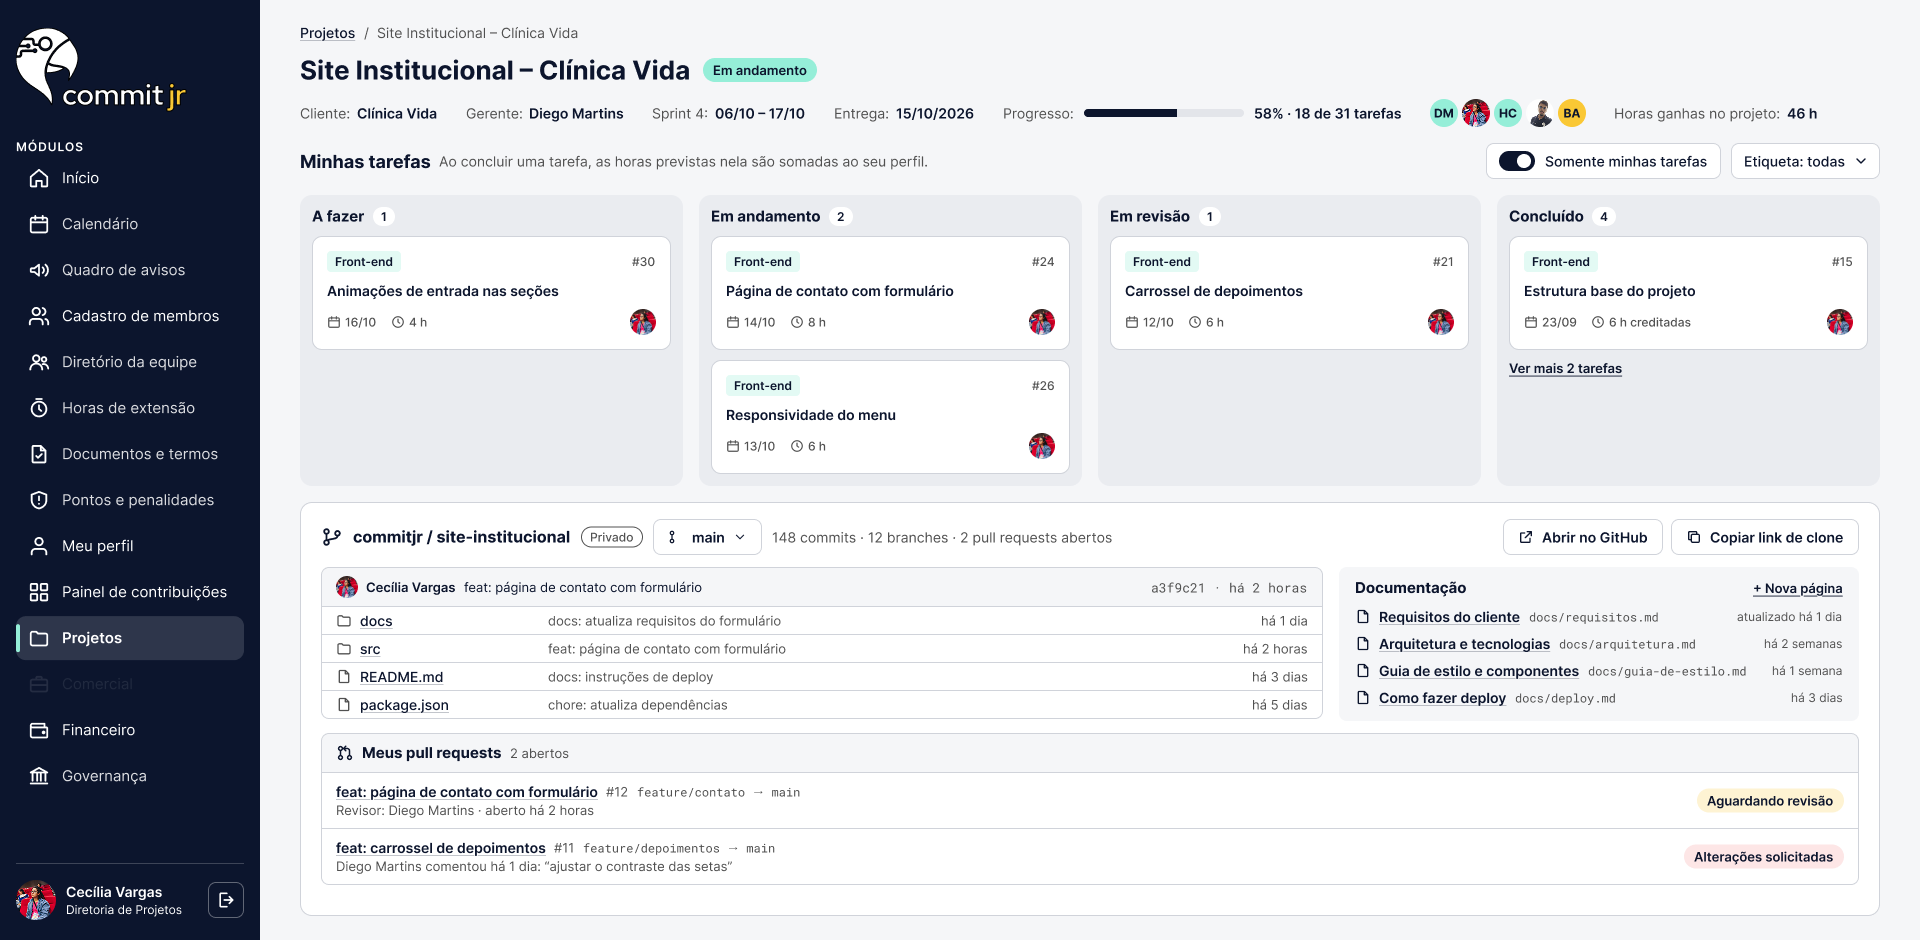
\includegraphics[width=0.88\textwidth]{Telas/projetos-visao-membro}} \\
\hline
\end{tabular}
\end{center}

\begin{center}
\begin{tabular}{|p{2.0cm}|p{11.5cm}|}
\hline
\textbf{PT-029} & \textbf{Gestão de Projetos - Lista de Tarefas do Membro} \\
\hline
\multicolumn{2}{|c|}{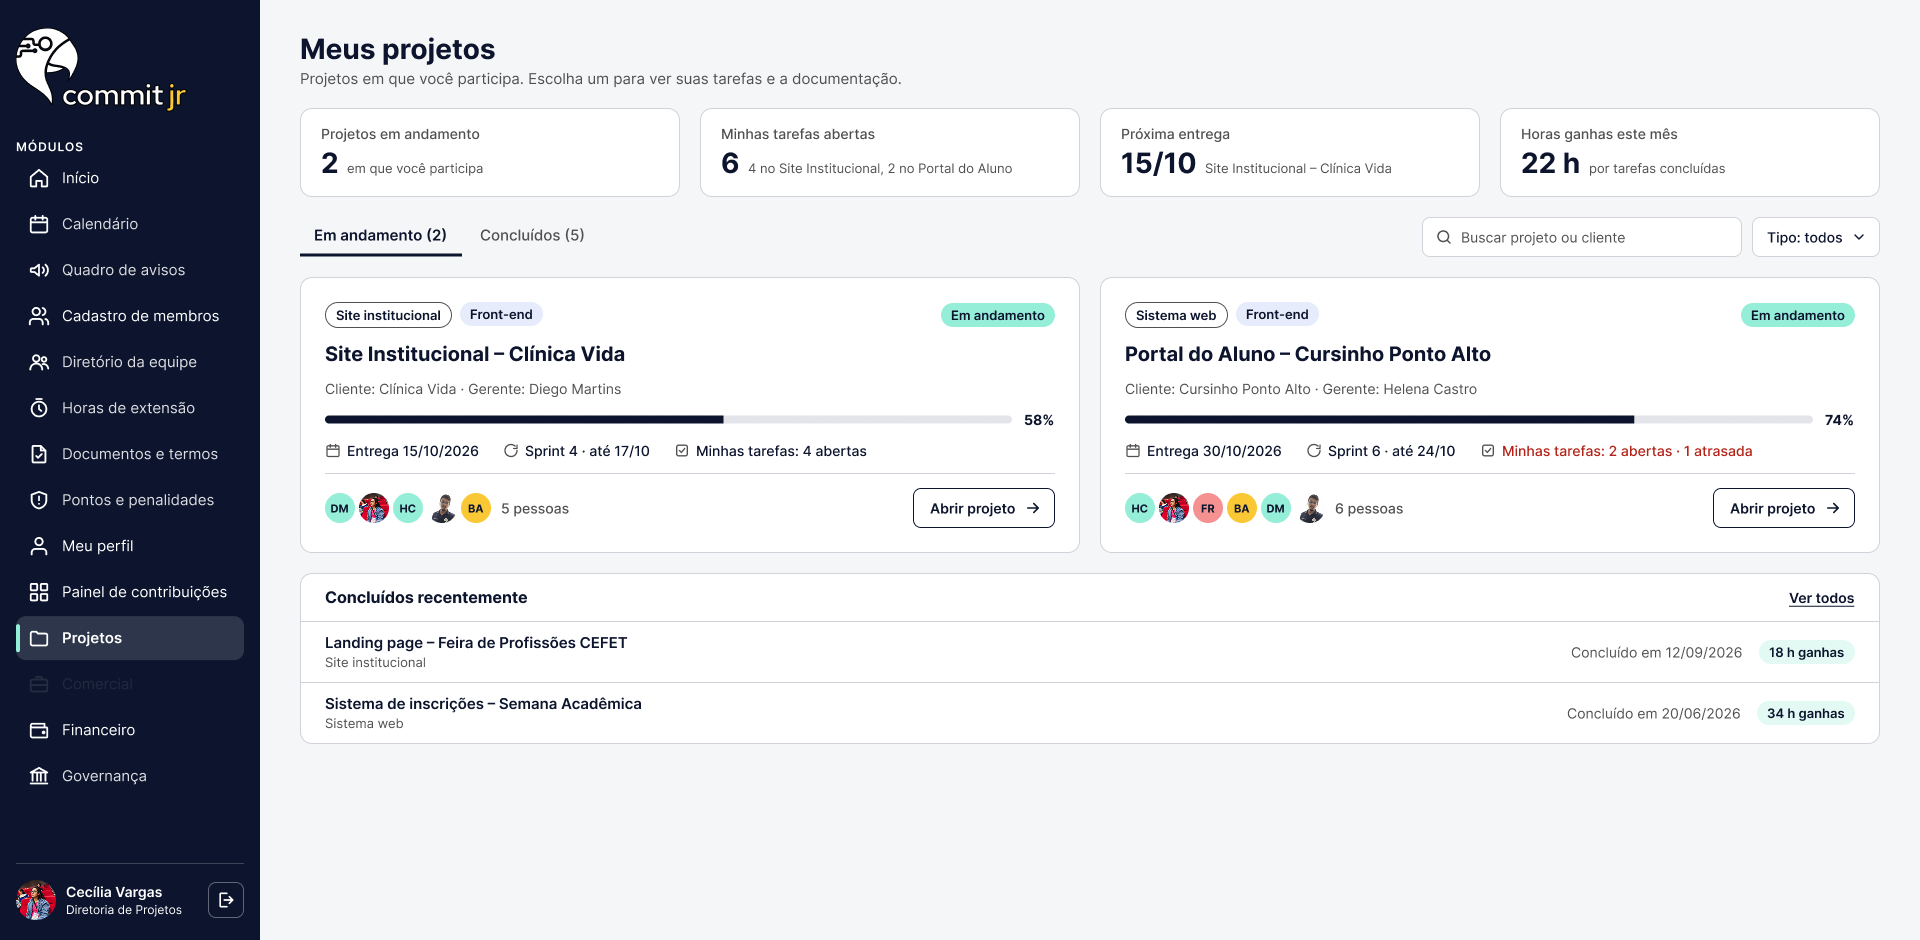
\includegraphics[width=0.88\textwidth]{Telas/projetos-lista-membro}} \\
\hline
\end{tabular}
\end{center}

\begin{center}
\begin{tabular}{|p{2.0cm}|p{11.5cm}|}
\hline
\textbf{PT-030} & \textbf{Gestão de Projetos - Cadastro de Nova Tarefa} \\
\hline
\multicolumn{2}{|c|}{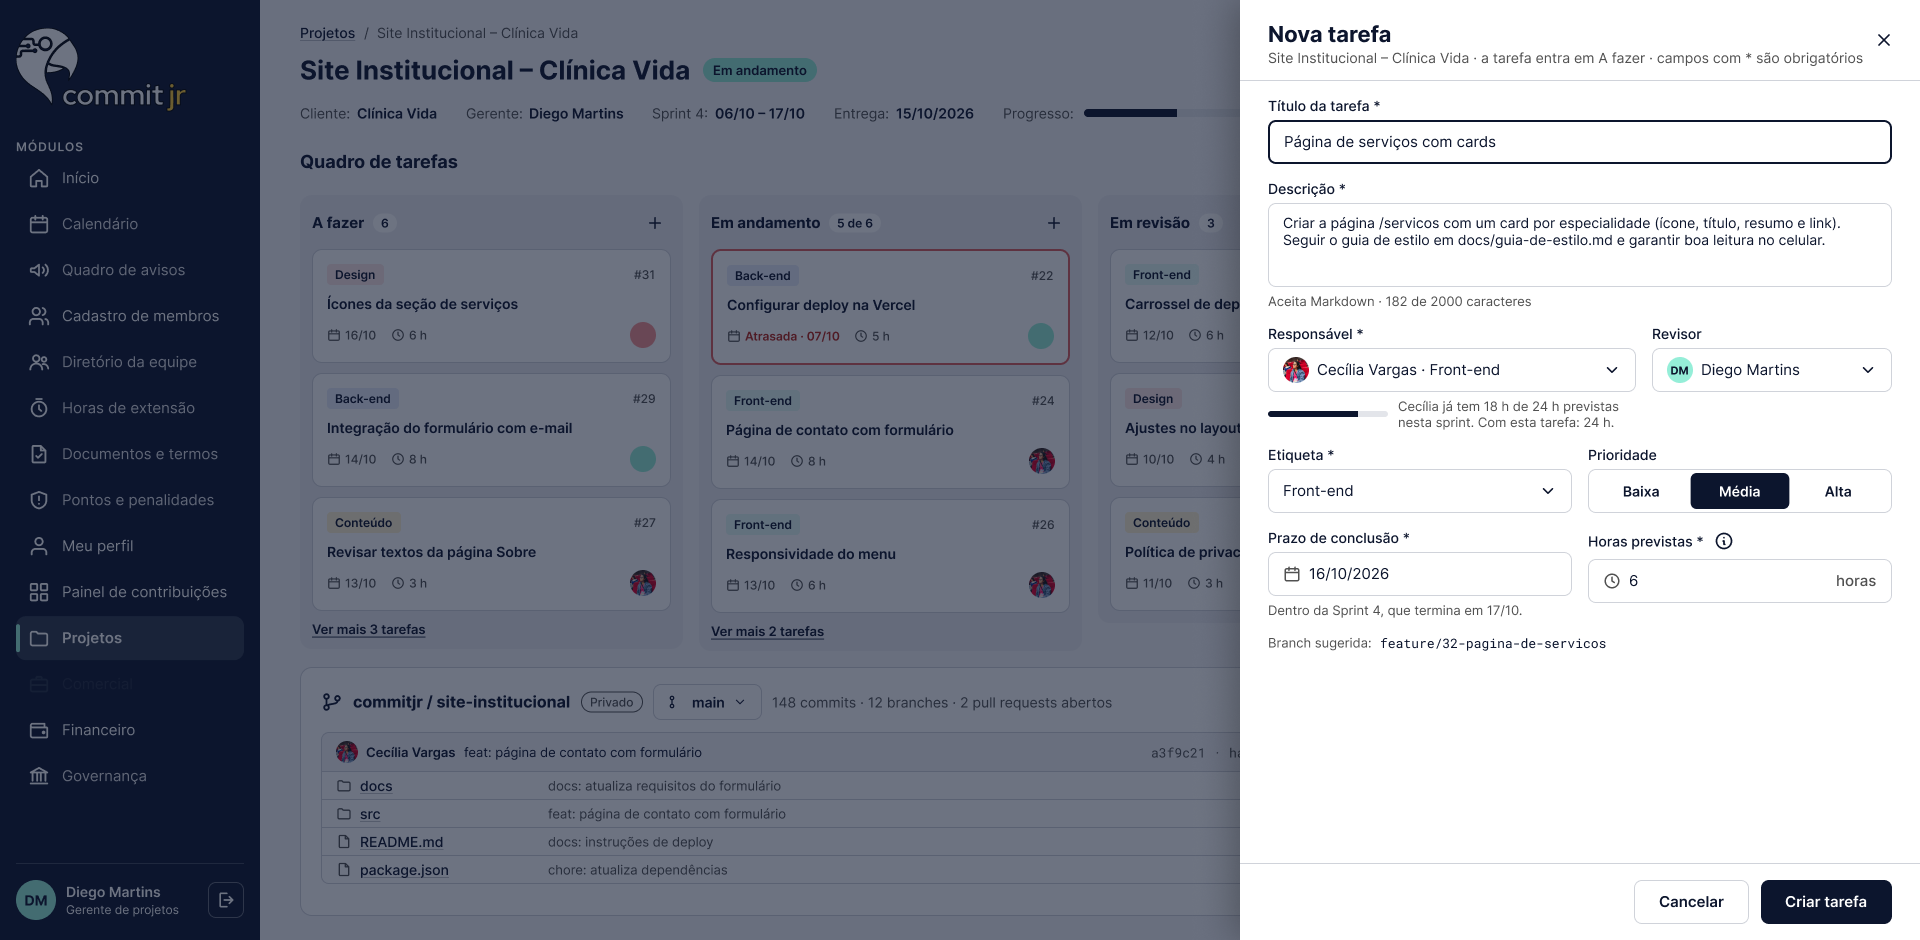
\includegraphics[width=0.88\textwidth]{Telas/projetos-nova-tarefa}} \\
\hline
\end{tabular}
\end{center}

\begin{center}
\begin{tabular}{|p{2.0cm}|p{11.5cm}|}
\hline
\textbf{PT-031} & \textbf{Gestão Comercial - Cadastro e Consulta de Clientes} \\
\hline
\multicolumn{2}{|c|}{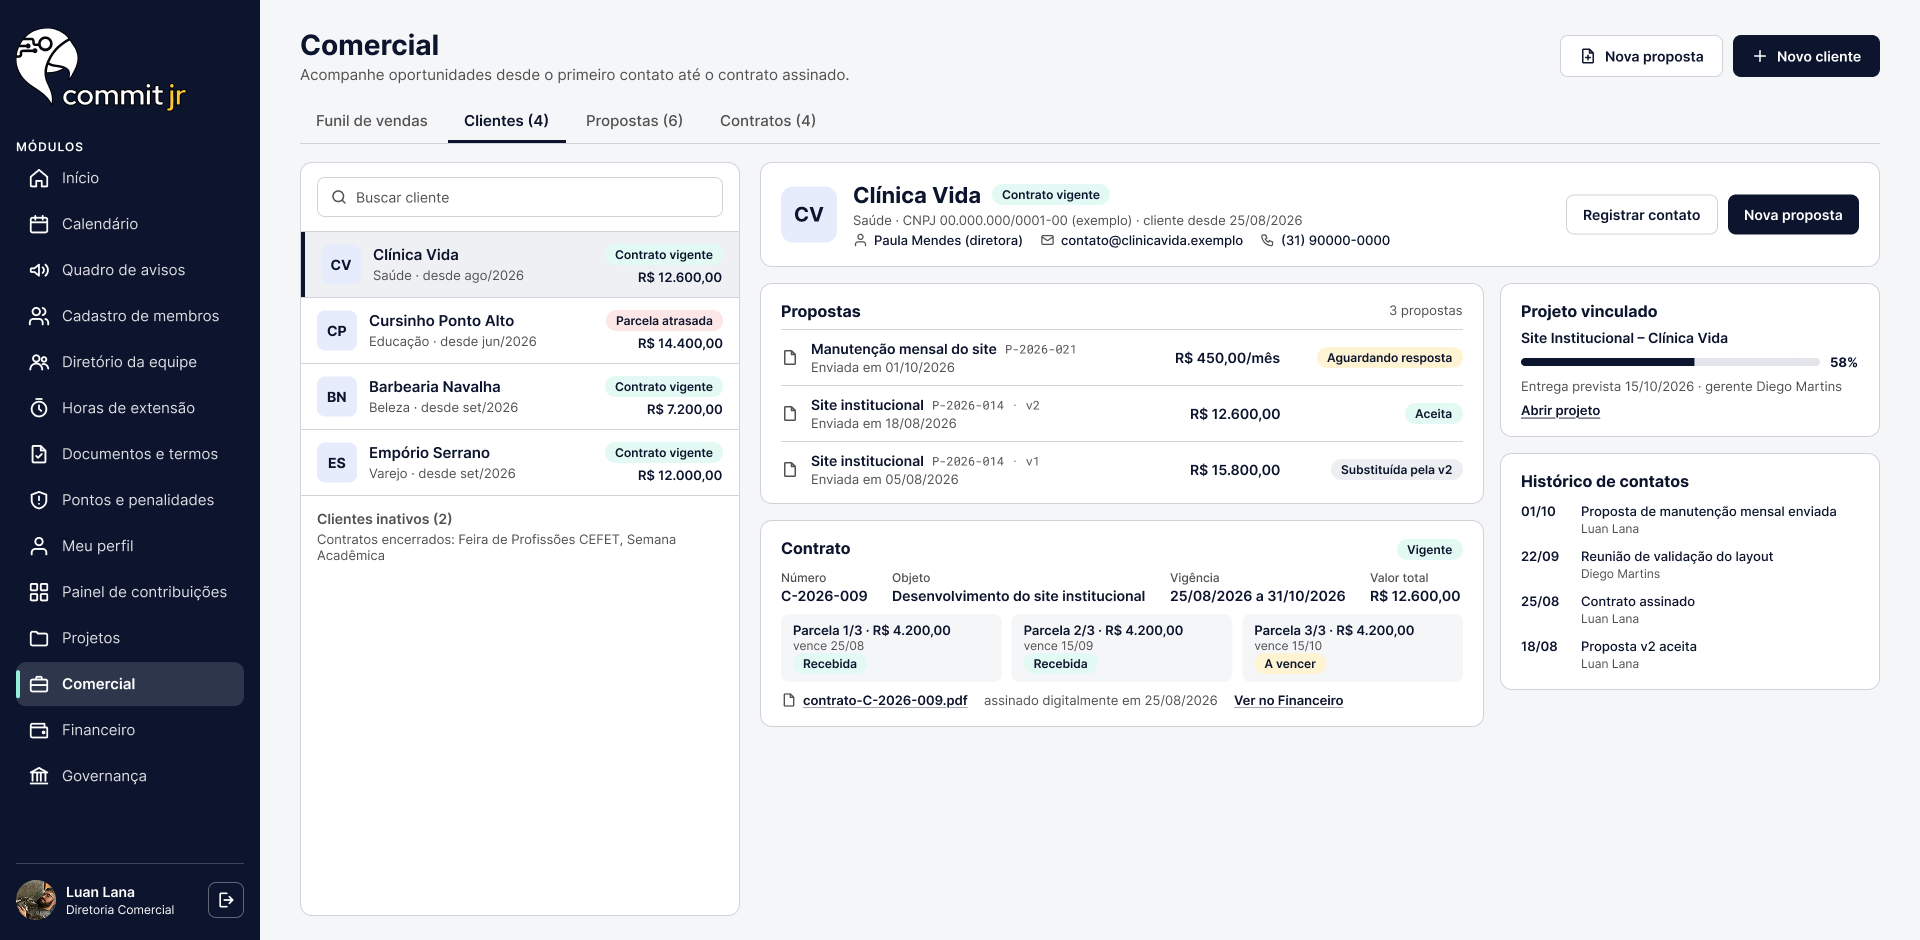
\includegraphics[width=0.88\textwidth]{Telas/comercial-clientes}} \\
\hline
\end{tabular}
\end{center}

\begin{center}
\begin{tabular}{|p{2.0cm}|p{11.5cm}|}
\hline
\textbf{PT-032} & \textbf{Gestão Comercial - Funil de Vendas} \\
\hline
\multicolumn{2}{|c|}{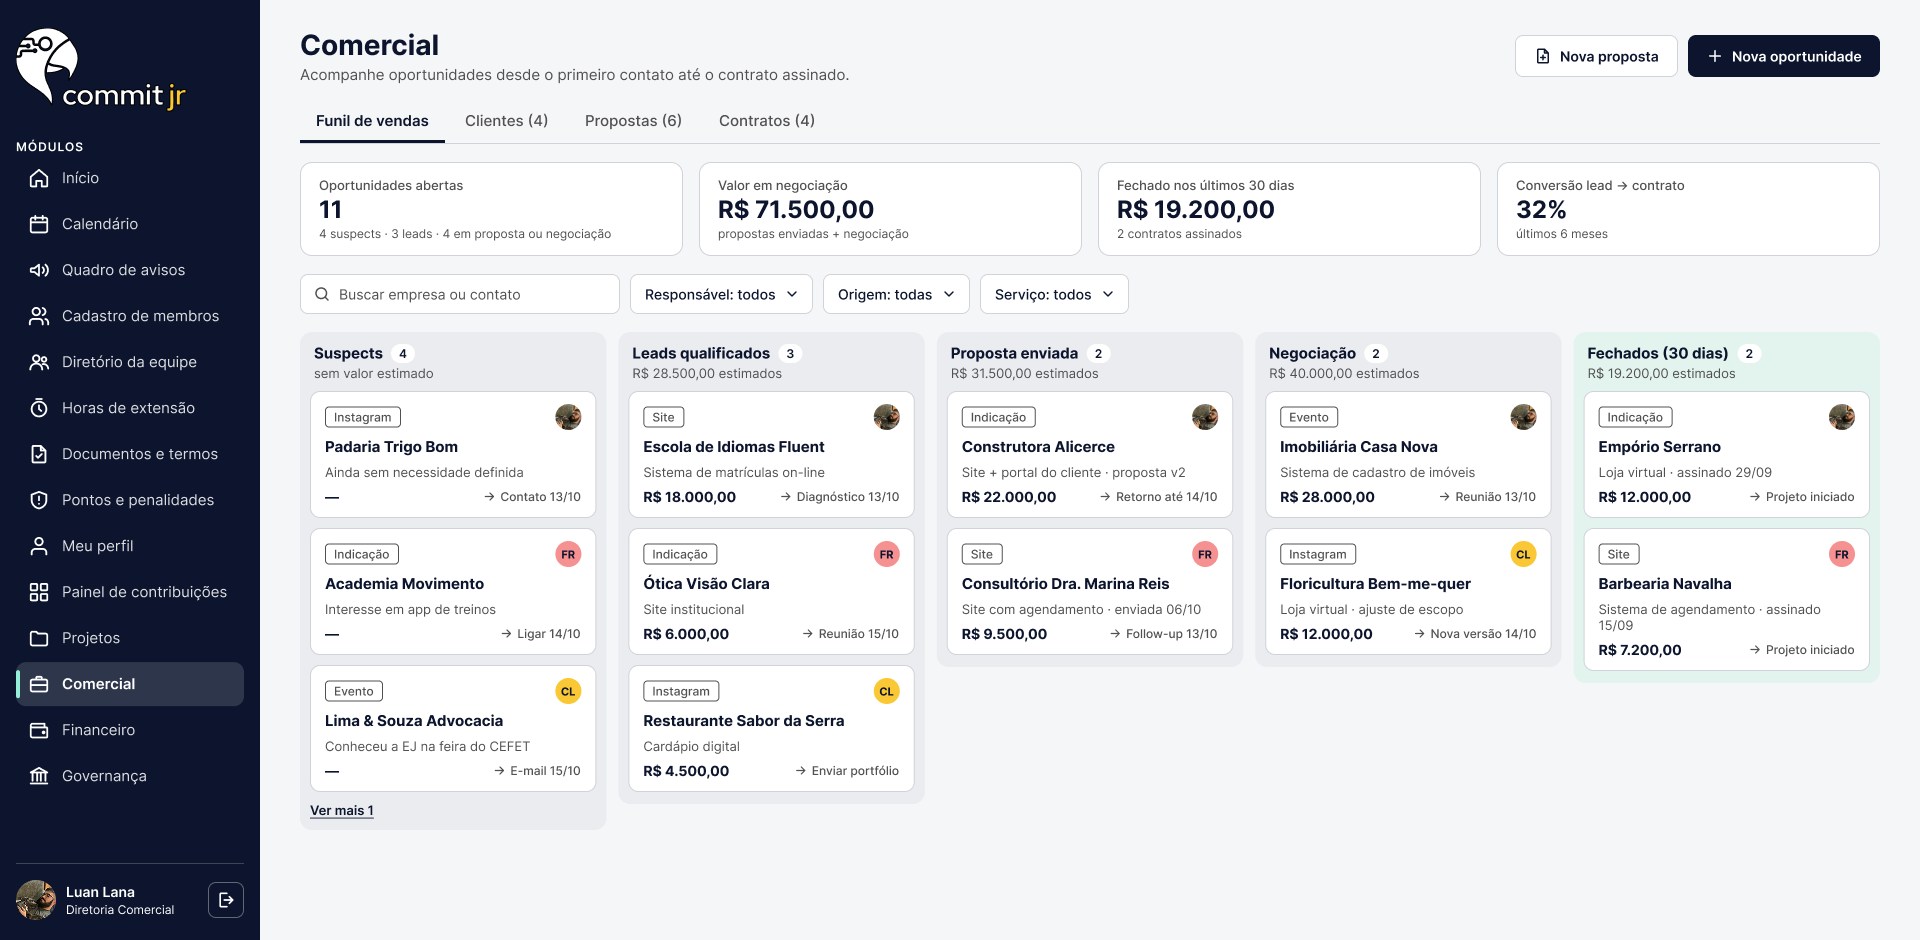
\includegraphics[width=0.88\textwidth]{Telas/comercial-funil-vendas}} \\
\hline
\end{tabular}
\end{center}

\begin{center}
\begin{tabular}{|p{2.0cm}|p{11.5cm}|}
\hline
\textbf{PT-033} & \textbf{Gestão Financeira - Visão Geral do Gerente} \\
\hline
\multicolumn{2}{|c|}{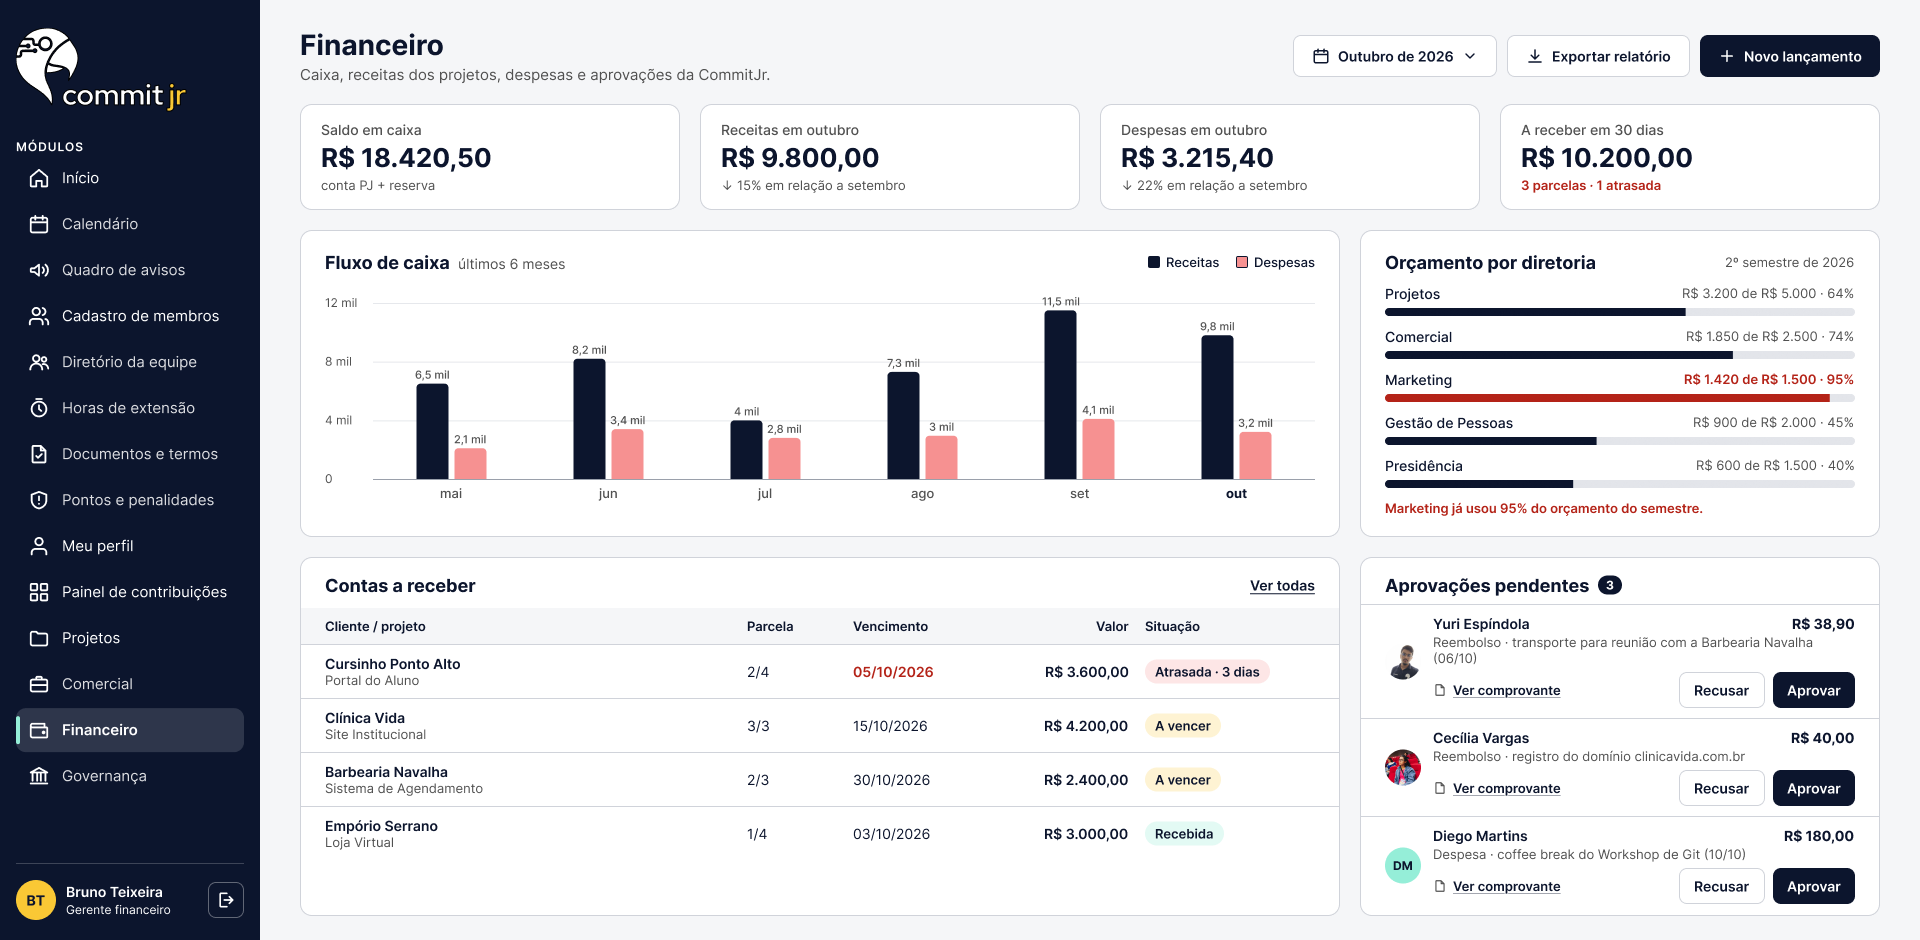
\includegraphics[width=0.88\textwidth]{Telas/financeiro-visao-geral}} \\
\hline
\end{tabular}
\end{center}

\begin{center}
\begin{tabular}{|p{2.0cm}|p{11.5cm}|}
\hline
\textbf{PT-034} & \textbf{Gestão Financeira - Novo Lançamento de Entrada} \\
\hline
\multicolumn{2}{|c|}{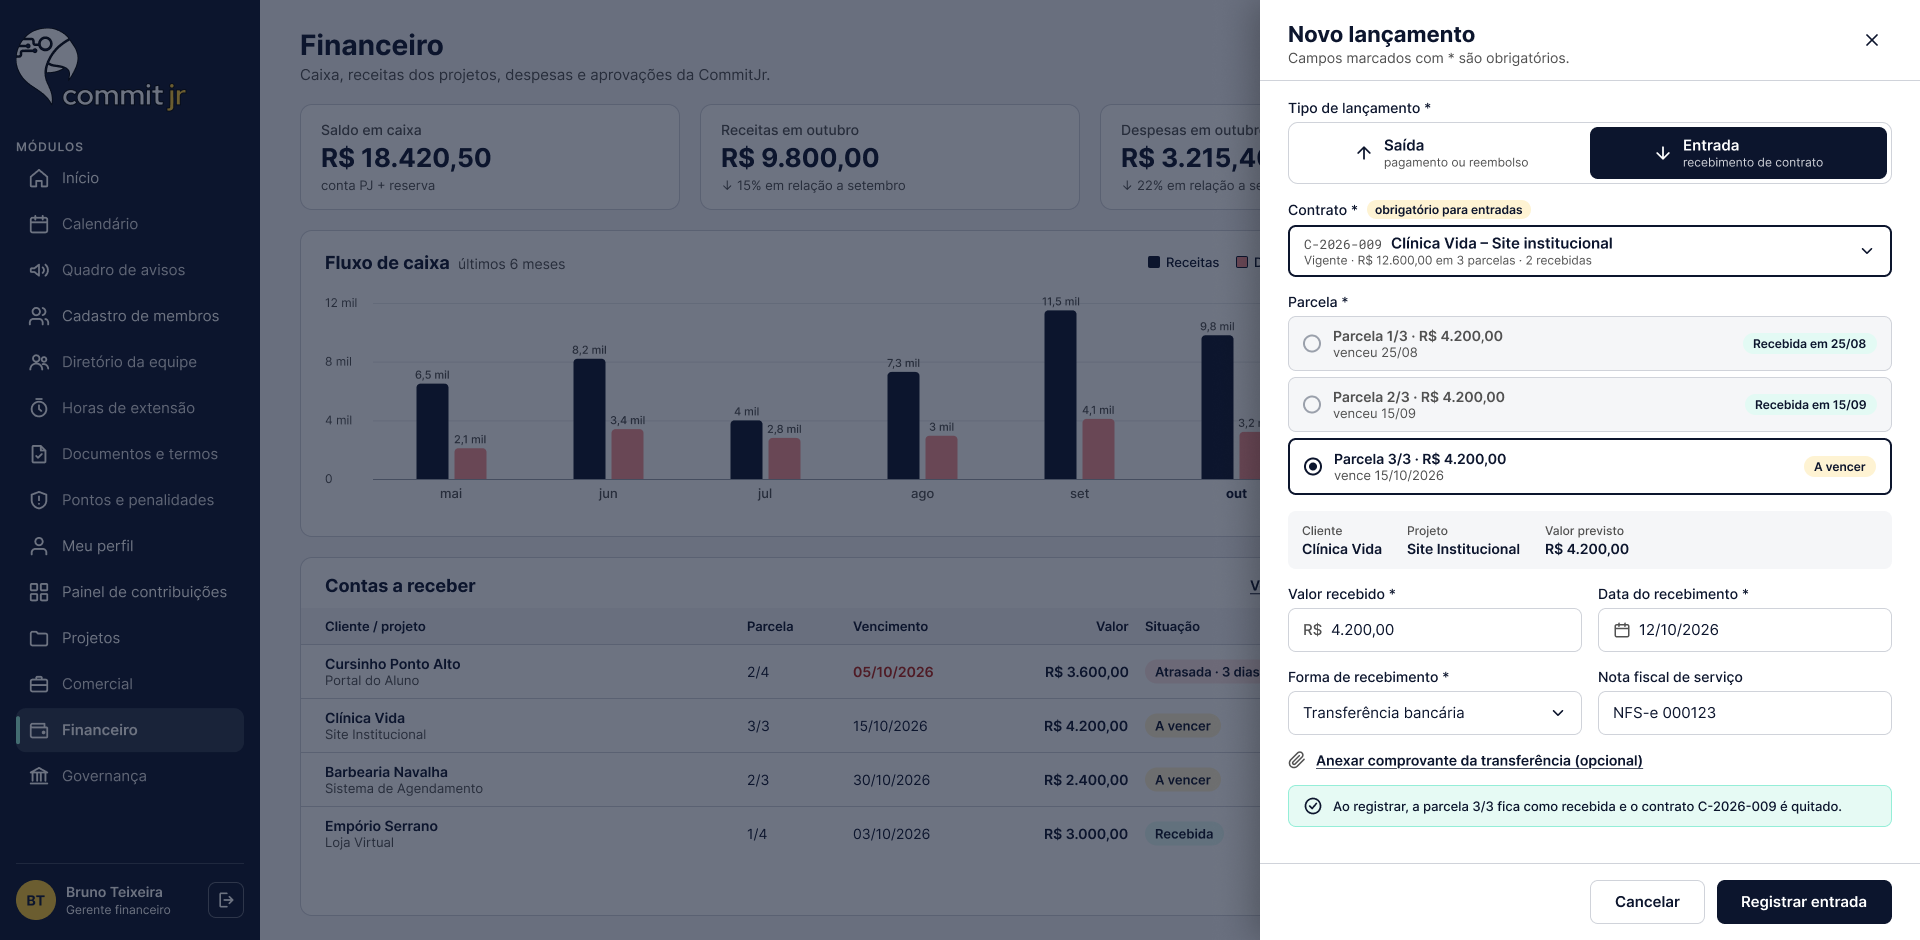
\includegraphics[width=0.88\textwidth]{Telas/financeiro-lancamento-entrada}} \\
\hline
\end{tabular}
\end{center}

\begin{center}
\begin{tabular}{|p{2.0cm}|p{11.5cm}|}
\hline
\textbf{PT-035} & \textbf{Gestão Financeira - Novo Lançamento de Saída} \\
\hline
\multicolumn{2}{|c|}{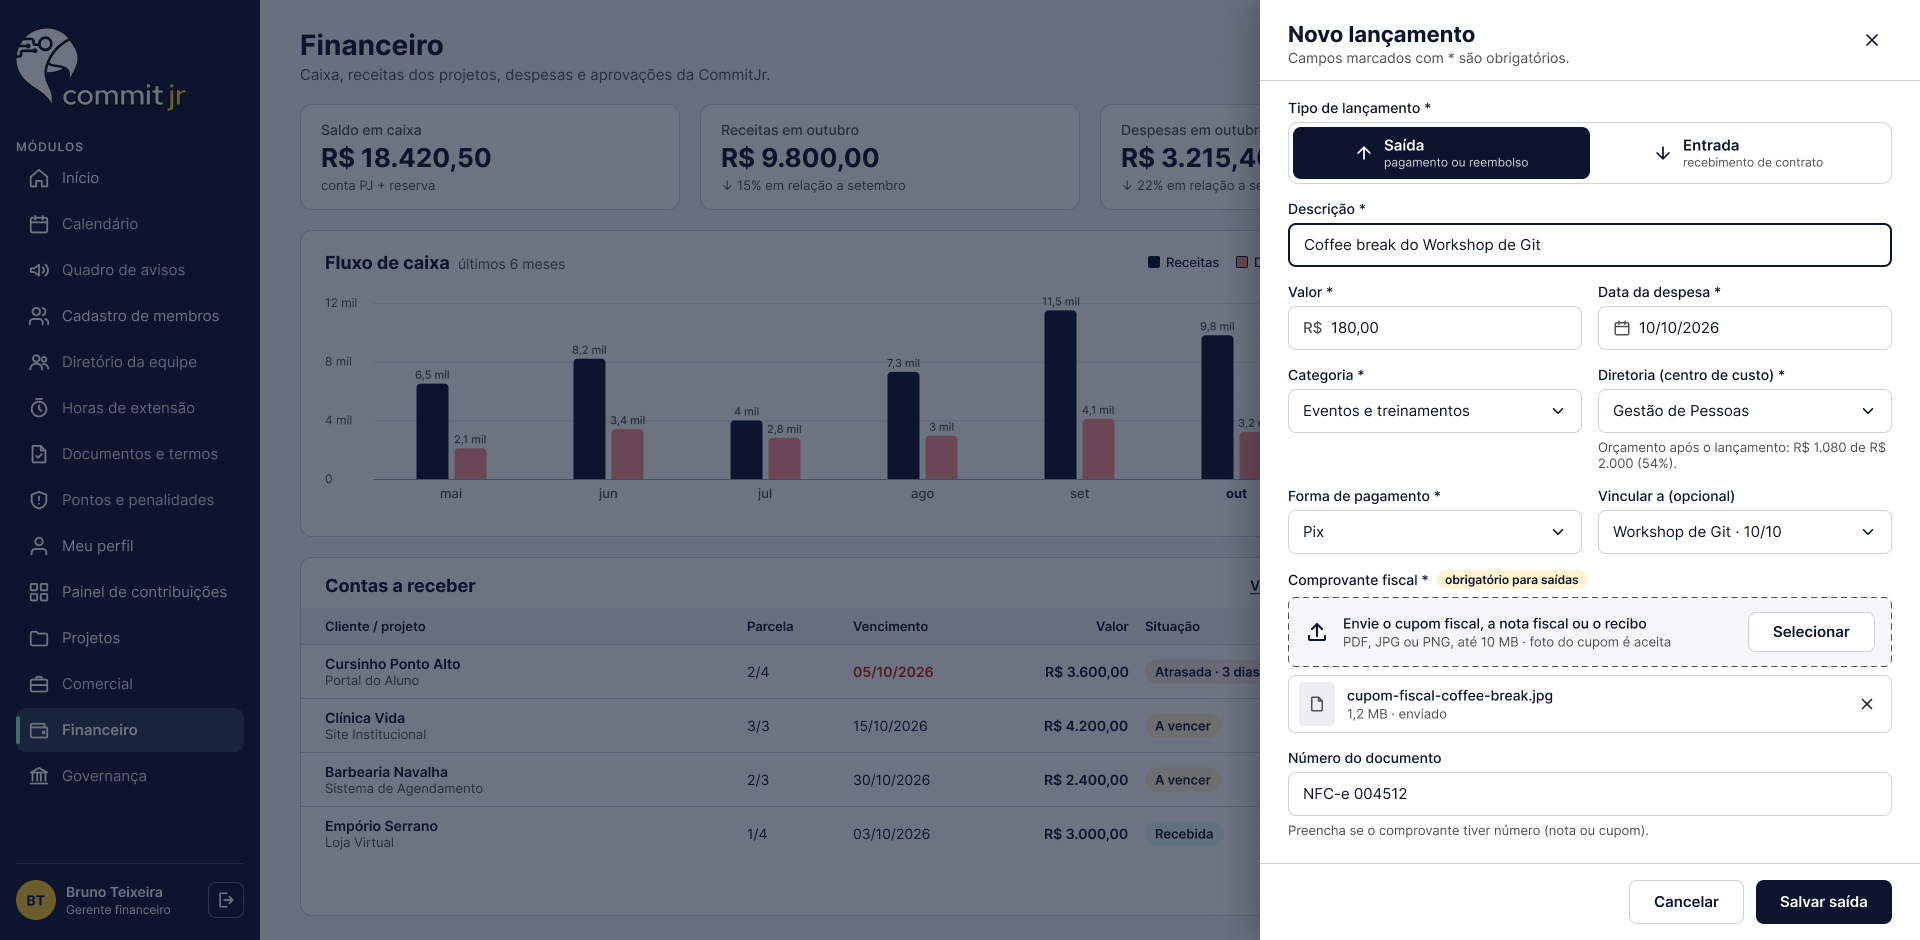
\includegraphics[width=0.88\textwidth]{Telas/financeiro-lancamento-saida}} \\
\hline
\end{tabular}
\end{center}

\clearpage
% ----------------------------------------------------------
% 7. Diagrama de Classes
% ----------------------------------------------------------
\chapter{Diagrama de Classes}
\label{cap:diagrama-classes}

Nesta seção é apresentado o Diagrama de Classes do sistema de gestão da Commit Júnior, elaborado sob a ótica da modelagem conceitual e lógica orientada a objetos[cite: 6, 20]. O diagrama foi modelado com o objetivo de refletir fielmente as entidades, relacionamentos, atributos e operações identificados ao longo do levantamento de requisitos, mantendo total rastreabilidade com o Minimundo, o Diagrama de Casos de Uso (DCU) e os protótipos de interface desenvolvidos[cite: 6, 20].

\begin{figure}[!htbp]
    \centering
    \caption[Diagrama de Classes do Sistema da Commit Júnior]{Diagrama de Classes do Sistema de Gestão de Membros da Commit Júnior}
    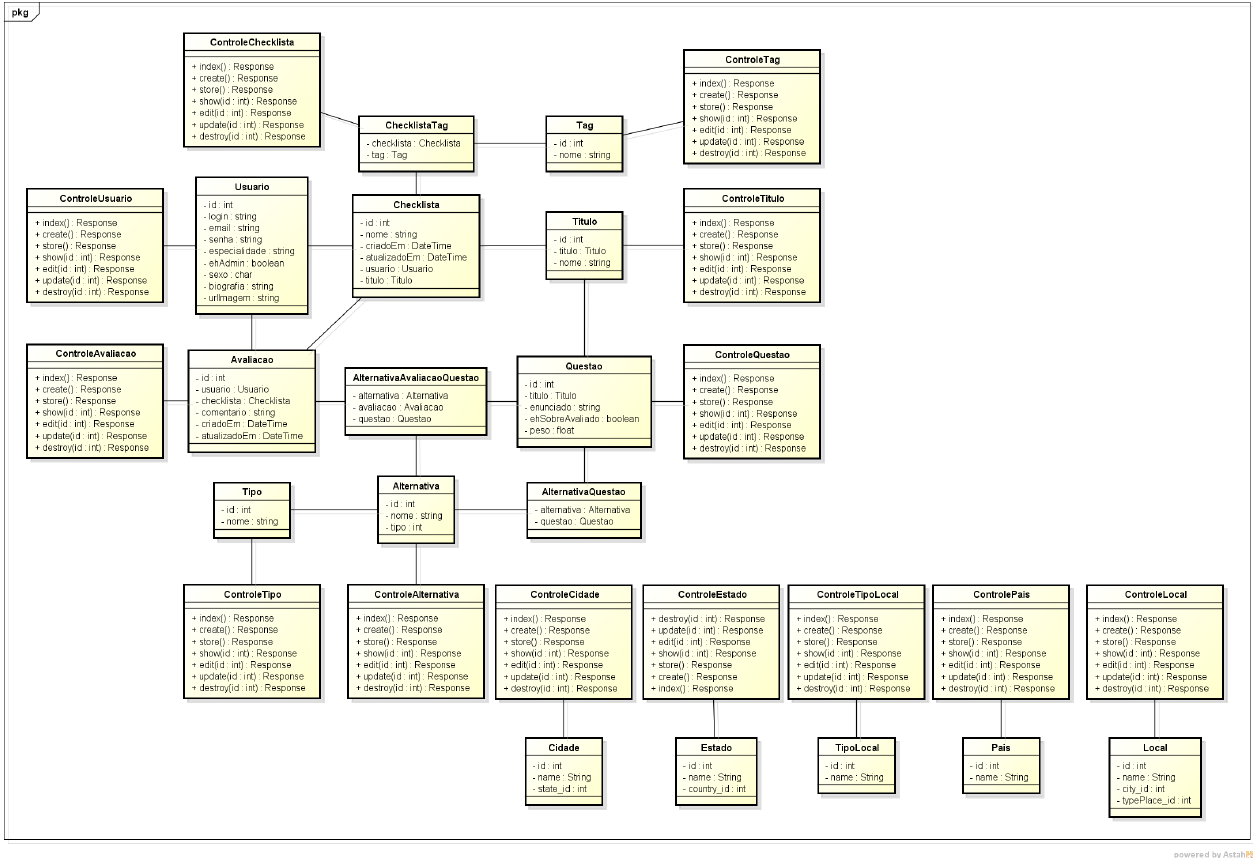
\includegraphics[width=0.98\textwidth,keepaspectratio]{exemplo-diagrama-classes.png}
    \label{fig:diagrama-classes}
\end{figure}

\section*{Descrição das Classes e Relacionamentos}

Para assegurar a completude e clareza da arquitetura de dados e domínio, as principais classes do modelo são descritas a seguir[cite: 20]:

\begin{itemize}
    \item \textbf{Membro:} Classe central do domínio que encapsula as informações cadastrais civis, acadêmicas e funcionais de cada integrante (como matrícula, CPF, RG, nome completo, curso, e-mail institucional, perfil de GitHub, status no sistema e data de ingresso)[cite: 1, 2, 4]. Implementa os métodos de controle de ciclo de vida e inativação lógica requeridos pelas regras de negócio[cite: 20].
    
    \item \textbf{Usuario / PerfilAcesso:} Responsável pelos mecanismos de autenticação, armazenamento seguro de credenciais (hash de senha) e autorização baseada em papéis (RBAC), segregando os privilégios entre Administrador, Jurídico, Líder de Área e Membro.
    
    \item \textbf{Cargo / Funcao e RegraHoras:} Entidades que parametrizam a estrutura organizacional (Diretoria, Squad) e definem a taxa de horas de extensão atribuída a cada atividade desempenhada por intervalo de vigência[cite: 1, 4].
    
    \item \textbf{HistoricoCargo / Extensao:} Associação temporal entre o membro e as funções desempenhadas, permitindo computar com precisão o tempo de permanência na empresa e o acumulado de horas de extensão para fins acadêmicos[cite: 1].
    
    \item \textbf{EnvioHorasCoordenacao:} Registra o lote de horas consolidadas que é gerado e despachado formalmente via correio eletrônico institucional (protocolo SMTP) ao professor orientador da Commit Júnior para homologação e lançamento no SIGAA[cite: 1].
    
    \item \textbf{TermoJuridico:} Gerencia os contratos obrigatórios de voluntariado, termos de rescisão/desligamento e certificados[cite: 2]. Mantém os códigos de autenticidade, links e o estado das assinaturas digitais intermediadas pelo serviço externo[cite: 2].
    
    \item \textbf{OcorrenciaPontuacao e Contestacao:} Modela o controle disciplinar da empresa júnior[cite: 3]. Registra infrações, saldo de pontos, prazos calculados de expiração e incidência de agravantes de reincidência, permitindo o acoplamento de justificativas formais abertas pelos membros[cite: 3].
    
    \item \textbf{Aviso:} Entidade responsável pelas publicações do mural de informes, admitindo segmentação geral institucional ou restrição por diretoria específica.
    
    \item \textbf{Compromisso / Evento:} Modela os compromissos corporativos plenários (Reuniões Gerais, imersões) e as reuniões individuais bilaterais (1-on-1), com validação de choques de horário entre os participantes.
\end{itemize}

\section*{Integração com Sistemas Externos}

Conforme especificado no Minimundo e nas regras de negócio, determinados dados e eventos interagem com plataformas e atores externos[cite: 20]:

\begin{itemize}
    \item \textbf{Autentique (Serviço de Assinatura Eletrônica):} Plataforma externa responsável pelo fluxo de coleta de assinaturas digitais nos termos contratuais e certificados[cite: 2]. O sistema armazena apenas a referência do documento, código de autenticação e status de retorno[cite: 2].
    
    \item \textbf{Servidor SMTP Institucional:} Subsistema de mensageria responsável pela entrega dos relatórios formais de extensão e comunicados de desligamento por e-mail[cite: 6].
    
    \item \textbf{SIGAA (CEFET-MG):} Sistema acadêmico institucional para o qual as horas de extensão aprovadas são transcritas pelo professor orientador da Commit Júnior[cite: 1]. O sistema proposto não realiza inserções diretas no banco de dados do SIGAA, atuando na geração dos demonstrativos auditáveis que subsidiam esse lançamento externo[cite: 1].
\end{itemize}

\clearpage
%% ----------------------------------------------------------
% 8. Arquitetura do Sistema
% ----------------------------------------------------------
\chapter{Arquitetura do Sistema}
\label{cap:arquitetura}

% ----------------------------------------------------------
\section{Diagrama de pacotes}
% ----------------------------------------------------------

\obs{Colocar aqui o Diagrama pacotes representando a arquitetura lógica do sistema
proposto pelo seu grupo.}

% ----------------------------------------------------------
\section{Diagrama de implantação}
% ----------------------------------------------------------

\obs{Colocar aqui o Diagrama de implantação representando a arquitetura física do
sistema proposto pelo seu grupo.}

%% ----------------------------------------------------------
% 9. Projeto de Dados
% ----------------------------------------------------------
\chapter{Projeto de Dados}
\label{cap:projeto-dados}

% ----------------------------------------------------------
\section{Modelo de dados do projeto}
% ----------------------------------------------------------

\obs{Colocar aqui o diagrama que representa o modelo de dados do projeto: o DER do seu
projeto (DER: Diagrama Entidade Relacionamento), ou o esquema de dados NOSQL etc. Ele
pode ser elaborado em ferramentas de modelagem UML ou gerados pelo ambiente de
desenvolvimento. (Deve existir em todos os projetos que envolvem banco de dados). O
exemplo abaixo é de um DER para vocês lembrarem como é.}

\begin{figure}[htb]
	\centering
	\caption[Exemplo de DER]{Exemplo de DER}
	\label{fig:exemplo-der}
	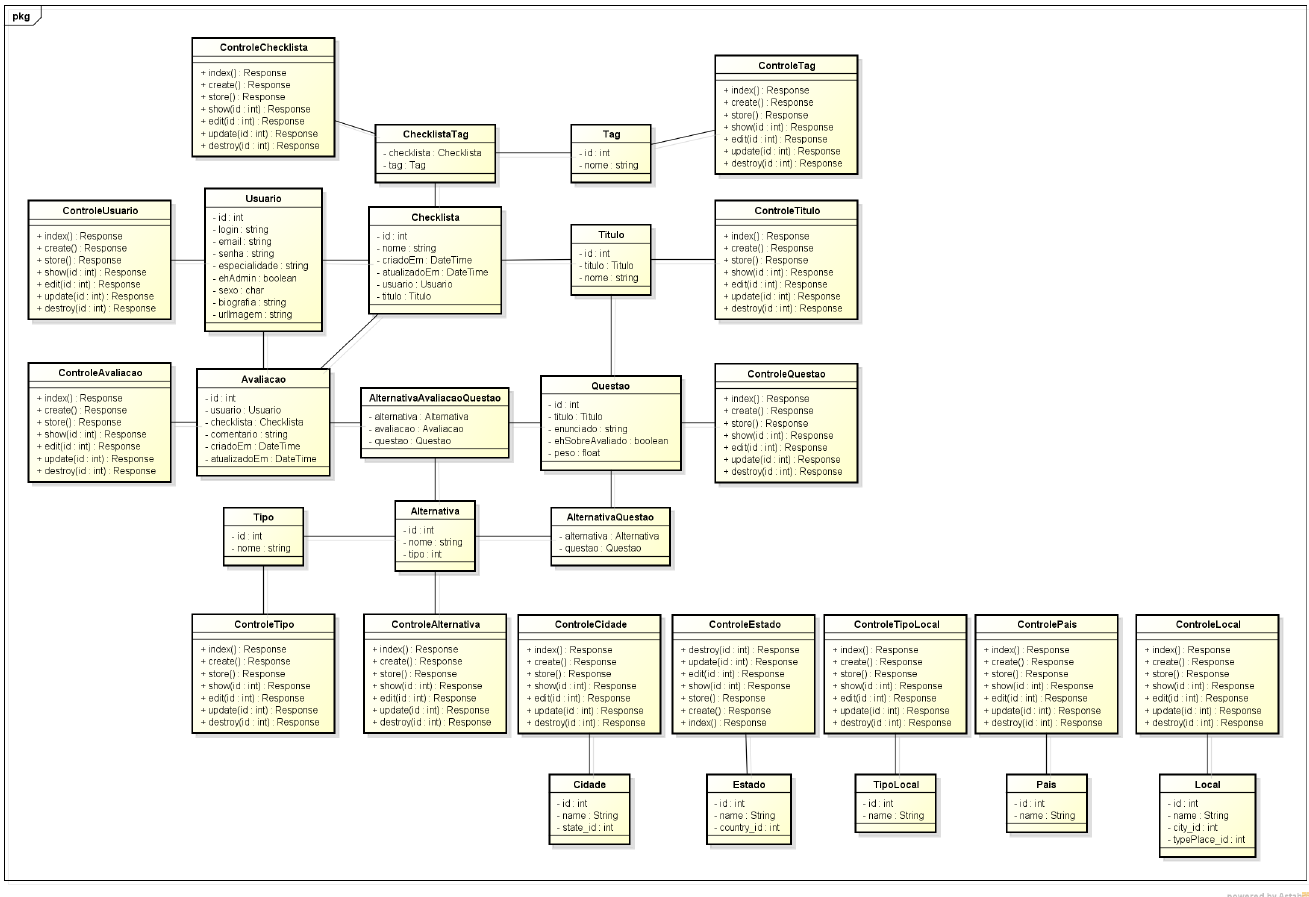
\includegraphics[width=\textwidth]{exemplo-der}
\end{figure}

% ----------------------------------------------------------
\section{Dicionário de Dados Completo}
% ----------------------------------------------------------

\obs{Faça um dicionário completo. O exemplo abaixo é para vocês lembrarem como é.}

% ---
% O documento original pede que as páginas do dicionário de dados fiquem em PAISAGEM.
% Isso é feito aqui pelo ambiente landscape (pacote pdflscape).
% ---
\begin{landscape}

\footnotesize

\noindent
\begin{tabular}{|p{4.0cm}|p{12.0cm}|p{5.0cm}|}
\hline
\textbf{ENTIDADE} & & \\
\hline
\textbf{Nome:} & \multicolumn{2}{p{17.4cm}|}{Tabela de Curso} \\
\hline
\textbf{Nome Abreviado:} & \multicolumn{2}{p{17.4cm}|}{TBCURSO} \\
\hline
\textbf{Índices:} & \textbf{Nome do Índice} & \textbf{Atributos} \\
\hline
 & IND\_TBCURSO\_NMCURSO & NMCURSO \\
\hline
\textbf{Descrição:} & \multicolumn{2}{p{17.4cm}|}{Tabela que contém todos os cursos
oferecidos pela Universidade Miranda} \\
\hline
\end{tabular}

\vspace{0.4cm}

\noindent\textbf{Atributos:}

\noindent
\begin{tabular}{|p{3.6cm}|c|c|p{7.0cm}|p{2.8cm}|p{3.0cm}|}
\hline
\textbf{Nome do Atributo} & \textbf{Tipo} & \textbf{Tamanho} & \textbf{Descrição} &
\textbf{Máscara} & \textbf{Regra Validação} \\
\hline
\textbf{\underline{CDCURSO}} & N & 5,0 & Código do Curso & 99.999 & >0 \\
\hline
NMCURSO & T & 50 & Nome do Curso & & Obrigatório \\
\hline
CDAREA & N & 5,0 & Código da Área & 99.999 & >0 \\
\hline
DTINCREG & D & 10 & Data Inclusão Registro & 99/99/9999 & < = date ( ) \\
\hline
CDUSUINC & N & 5,0 & Código Usuário Incluiu Registro & 99.999 & >0 \\
\hline
DTALTREC & D & 8 & Data Alteração do Registro & 99/99/9999 & < = date ( ) \\
\hline
CDUSUALT & N & 5,0 & Código Usuário Alterou Registro & 99.999 & >0 \\
\hline
\end{tabular}

\vspace{1.0cm}

\noindent
\begin{tabular}{|p{4.0cm}|p{12.0cm}|p{5.0cm}|}
\hline
\textbf{ENTIDADE} & & \\
\hline
\textbf{Nome:} & \multicolumn{2}{p{17.4cm}|}{Cadastro de Aluno} \\
\hline
\textbf{Nome Abreviado:} & \multicolumn{2}{p{17.4cm}|}{TBALUNO} \\
\hline
\textbf{Índices:} & \textbf{Nome do Índice} & \textbf{Atributos} \\
\hline
 & IND\_TBALUNO\_NMALUNO & NMALUNO \\
\hline
 & IND\_TBALUNO\_CPF & CPF \\
\hline
\textbf{Descrição:} & \multicolumn{2}{p{17.4cm}|}{Tabela que contém todos os alunos
matriculados na Universidade Miranda} \\
\hline
\end{tabular}

\vspace{0.4cm}

\noindent\textbf{Atributos:}

\noindent
\begin{tabular}{|p{3.6cm}|c|c|p{7.0cm}|p{2.8cm}|p{3.0cm}|}
\hline
\textbf{Nome do Atributo} & \textbf{Tipo} & \textbf{Tamanho} & \textbf{Descrição} &
\textbf{Máscara} & \textbf{Regra Validação} \\
\hline
\textbf{\underline{CDALUNO}} & N & 5,0 & Código do Aluno & 99.999 & >0 \\
\hline
NMALUNO & T & 50 & Nome do Aluno & & Obrigatório \\
\hline
SEXO & T & 1 & Sexo & & \\
\hline
CDCURSO & N & 5,0 & Código do Curso & 99.999 & >0 \\
\hline
CDCIDADENASC & N & 5,0 & Código Cidade Nascimento & 99.999 & >0 \\
\hline
CDCIDADERES & N & 5,0 & Código Cidade Residência & 99.999 & >0 \\
\hline
EDFONE & T & 10 & Telefone & (99)9999-9999 & \\
\hline
CPF & N & 11 & CPF do Aluno & 999.999.999-99 & obrigatório \\
\hline
DTINCREG & D & 8 & Data Inclusão Registro & 99/99/9999 & < = date ( ) \\
\hline
CDUSUINC & N & 5,0 & Código Usuário Incluiu Registro & 99.999 & >0 \\
\hline
DTALTREC & D & 8 & Data Alteração do Registro & 99/99/9999 & < = date ( ) \\
\hline
CDUSUALT & N & 5,0 & Código Usuário Alterou Registro & 99.999 & >0 \\
\hline
\end{tabular}

\normalsize
\end{landscape}


\bookmarksetup{startatroot}

\postextual

\nocite{bezerra2015}
\bibliography{bibfile}

\end{document}